\chapter{Random Simplicial Complexes}
\label{ch:random}
In this chapter we carry out some experiments regarding apparent pairs on random simplicial complexes. We will consider two different notions of random simplicial complexes. Namely, alpha complexes constructed on randomly generated point clouds and two-dimensional analogues of the Erdös--Rényi random graph model as introduced by Meshulam and Linial in \cite{LinialMeshulam} and extended by Meshulam and Wallach in \cite{Meshulam_Wallach_2009}. An extensive discussion of results regarding these was done by Kahle in \cite{kahle2016random}. For some insights and experiments regarding apparent pairs and Vietoris--Rips complexes see \cite{bauer2019ripser}.

\section{Erdös--Rényi Analogues}
Consider the set $G(n)$ of all graphs on vertex set $\{1,\dots,n\}$. The Erdös--Rényi random graph model $G(n,p)$ is the probability distribution on $G(n)$, \enquote{where every edge is included with probability $p$ jointly independently.} \cite{kahle2016random}[page 1].

A general analogue in terms of simplicial complexes is the random $k$-complex $Y_k(n,p)$ introduced in \cite{Meshulam_Wallach_2009}. $Y_k(n,p)$ \enquote{contains the complete $(k-1)$-skeleton of a simplex on $n$ vertices, and every $k$-dimensional face appears independently with probability $p$.} \cite{kahle2016random}[page 4].

In our case $Y_k(n,p)$ will have $n+1$ vertices since we want to keep it consistent with our previous notations for filtrations.

We will construct filtrations by ordering simplices by dimension first and lexicographically within the respective dimensions. Then we take the full $(k-1)$-skeleton in that order. Finally we include each $k$-face with probability $p$. 
The following Figure \ref{fig:randomk} gives an example of a random $2$-complex on four points, i.e., for $n=3$.

\begin{figure}[H]
%\centering%
\begin{subfigure}[b]{0.99\textwidth}
\begin{center}
\begin{tikzpicture}

\node[b_circle, name path=0, label=below:{0}] (0) at (0,0) {};

\node[b_circle, name path=1, label=below:{1}] (1) at (4,0) {};

\node[b_circle, name path=2, label=above:{2}] (2) at  (2,4) {};

\node[b_circle, name path=2, label=above left:{3}] (3) at  (2,1.5) {};


\draw[thick] (0) to (1);
\draw[thick] (0) to (2);
\draw[thick] (0) to (3);

\draw[thick] (1) to (2);
\draw[thick] (1) to (3);
\draw[thick] (2) to (3);

\fill[opacity = 0.2] (0.center) -- (1.center) -- (3.center);
\fill[opacity = 0.2] (2.center) -- (1.center) -- (3.center);

\end{tikzpicture}
\end{center}
\end{subfigure}
\caption{Random $2$-complex on four points.}
\label{fig:randomk}
\end{figure}

We have not explicitly stated a value for $p$ with respect to Figure \ref{fig:randomk}, since the complex might result from any $p > 0$ with varying probability. The corresponding filtration is \[
F_* = ([0],[1],[2],[3],[0,1],[0,2],[0,3],[1,2],[1,3],[2,3],[0,1,3],[1,2,3]).
\]


\section{Apparent Pairs on Random 2-Complexes}
In this section we will analyze apparent pairs in the context of random $2$-complexes $Y_2(n,p)$ for fixed $n$ and varying $p$. We consider filtrations as specified in the previous section.

An interesting observation is that for $n\in \mathbb{N}$, $p \in \{0,1\}$, and simplices of $Y_2(n,p)$ in lexicographical order, the apparent gradient always yields a perfect Morse matching. 

For $p = 0$ and $n$ arbitrary but fixed we get the following filtration: 
\[
F_* = ([0],[1],\dots,[n],[0,1],\dots,[0,n],[1,2],\dots,[n-1,n]).
\]
Looking at the apparent pairs we see that $[0]$ is not paired, i.e., is a critical cell. Vertex $[1]$ gets paired with $[0,1]$, $[2]$ gets paired with $[0,2]$, and so on until $[n]$ gets paired with $[0,n]$. All other edges remain unpaired, and there are no triangles or higher-dimensional faces. Furthermore, each edge that does not get paired, corresponds to a one-dimensional hole in the simplicial complex. Therefore, we get that the number of critical cells is equal to the Betti number in the respective dimensions. 

If $p = 1$, every edge that is not paired with a vertex gets paired with a triangle. Edge $[1,2]$ is the youngest facet of triangle $[0,1,2]$ which is the oldest cofacet of $[1,2]$. The same holds for $[1,3]$ and $[0,1,3]$ and so on until we reach $[1,n]$ and $[0,1,n]$. Then $[2,3]$ to $[2,n]$ get paired with $[0,2,3]$ to $[0,2,n]$. This pattern continues until $[n-1,n]$ gets paired with $[0,n-1,n]$. This means all vertices get paired with the edge between this vertex and $[0]$, while all edges that do not contain vertex $[0]$ get paired with the triangle containing this edge and vertex $[0]$.

For the following figure we sample $Y_2(10,p)$ for $p = 0,0.01,\dots,0.99,1$, calculate the Betti numbers for the resulting complex and subtract the number of critical cells in the apparent gradients. Then we count how often this difference equals zero and divide it by the total number of generated complexes, i.e., we calculated the ratio of the apparent gradient being a perfect Morse matching for different values of $p$. For each $p$ we constructed $1000$ simplicial complexes to average over.

\begin{figure}[H]
%\centering%
\begin{subfigure}[c]{0.95\textwidth}
\begin{center}
% This file was created by tikzplotlib v0.9.2.
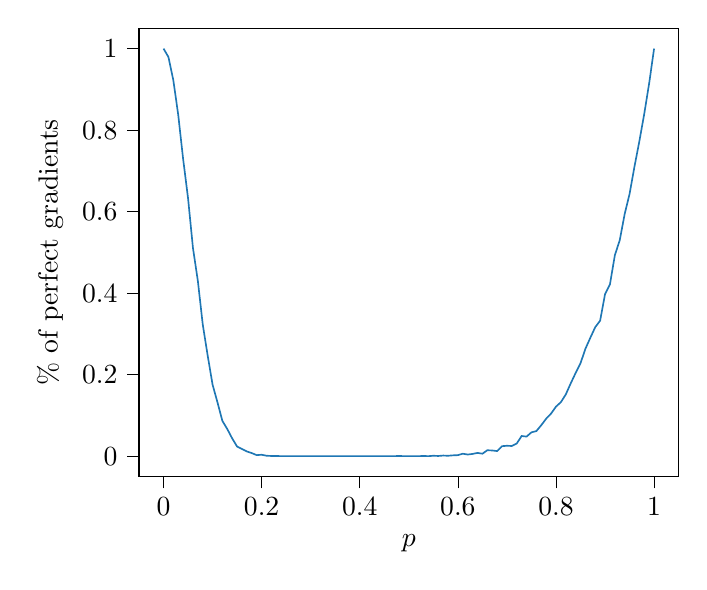
\begin{tikzpicture}

\definecolor{color0}{rgb}{0.12156862745098,0.466666666666667,0.705882352941177}

\begin{axis}[
tick align=outside,
tick pos=left,
xlabel = $p$,
ylabel = $\%$ of perfect gradients, 
x grid style={white!69.0196078431373!black},
xmin=-0.05, xmax=1.05,
xtick style={color=black},
y grid style={white!69.0196078431373!black},
ymin=-0.05, ymax=1.05,
ytick style={color=black}
]
\addplot [semithick, color0]
table {%
0 1
0.01 0.9795
0.02 0.9225
0.03 0.8375
0.04 0.729
0.05 0.633
0.06 0.511
0.07 0.43
0.08 0.323
0.09 0.247
0.1 0.1755
0.11 0.132
0.12 0.0865
0.13 0.0665
0.14 0.0435
0.15 0.0235
0.16 0.0175
0.17 0.0115
0.18 0.0075
0.19 0.0025
0.2 0.0035
0.21 0.001
0.22 0.0005
0.23 0.0005
0.24 0
0.25 0
0.26 0
0.27 0
0.28 0
0.29 0
0.3 0
0.31 0
0.32 0
0.33 0
0.34 0
0.35 0
0.36 0
0.37 0
0.38 0
0.39 0
0.4 0
0.41 0
0.42 0
0.43 0
0.44 0
0.45 0
0.46 0
0.47 0
0.48 0.0005
0.49 0
0.5 0
0.51 0
0.52 0
0.53 0.0005
0.54 0
0.55 0.001
0.56 0.0005
0.57 0.0015
0.58 0.001
0.59 0.002
0.6 0.0025
0.61 0.006
0.62 0.004
0.63 0.0055
0.64 0.008
0.65 0.006
0.66 0.0145
0.67 0.014
0.68 0.0125
0.69 0.0245
0.7 0.0255
0.71 0.025
0.72 0.031
0.73 0.0495
0.74 0.048
0.75 0.0585
0.76 0.0615
0.77 0.076
0.78 0.092
0.79 0.1045
0.8 0.1215
0.81 0.1325
0.82 0.1515
0.83 0.1785
0.84 0.204
0.85 0.228
0.86 0.2635
0.87 0.2905
0.88 0.3165
0.89 0.3325
0.9 0.3975
0.91 0.4215
0.92 0.493
0.93 0.53
0.94 0.594
0.95 0.6435
0.96 0.7105
0.97 0.773
0.98 0.8405
0.99 0.9155
1 1
};
\end{axis}

\end{tikzpicture}

\end{center}
\end{subfigure}
\caption{Probability of the apparent gradient being a perfect Morse matching for $Y_2(10,p)$ with different values of $p$.}
\label{fig:perfect_apparent}
\end{figure}

As we have previously argued for $p = 0$ the apparent gradient is perfect. In order for an apparent gradient to be not perfect, the number of critical cells in some dimension $l$ has to be larger than the Betti number $\beta_l$.

This can happen for example, if two triangles $[a,b,c]$ and $[b,c,d]$ have edge $[b,c]$ as a youngest facet but $[b,c]$ can only have one of them as the oldest cofacet. Without loss of generality it is $[a,b,c]$. This means that triangle $[b,c,d]$ is critical, i.e., the number of critical cells in dimension two is higher than $\beta_2$. Furthermore there also has to be some edge which can not be paired, hence the number of critical edges equals $\beta_1 + 1$. Up to a certain point it holds that the higher number of simplices in a complex drawn from $Y_2(10,p)$ causes situations to occur in which triangles can not be paired. This could explain the inital decline of the curve. 

If more and more simplices appear, we get closer to the structure of the full simplex in which the apparent gradient is a perfect Morse matching again, hence the increase after $p = 0.6$.

For the next figure we compute
\[
	d = \sum_{i=0}^2 c_i - \sum_{i=0}^2 \beta_i,
\] for each sampled complex. Here $c_i$ is the number of critical cells in dimension~$i$. We average these values over $1000$ sampled complexes for $Y_2(10,p)$ and $200$ sampled complexes for $Y_2(15,p)$ and $Y_2(20,p)$.

\begin{figure}[H]
%\centering%
\begin{subfigure}[c]{0.95\textwidth}
\begin{center}
% This file was created by tikzplotlib v0.9.2.
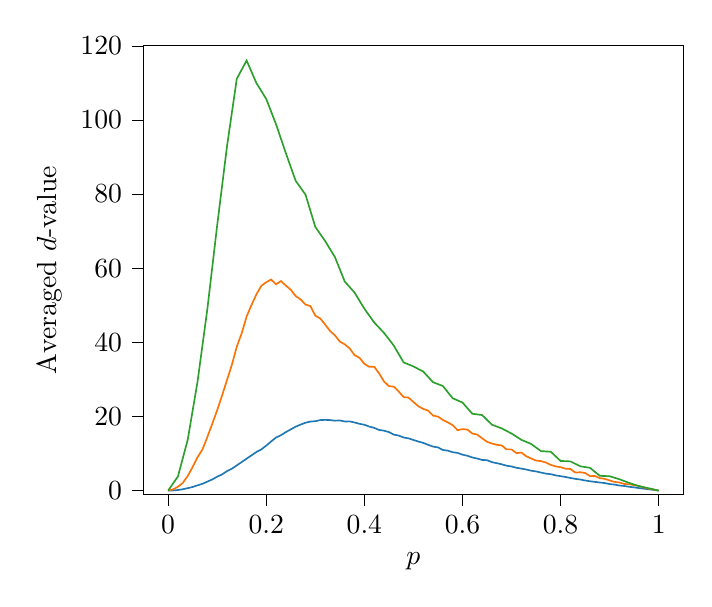
\begin{tikzpicture}

\definecolor{color0}{rgb}{0.12156862745098,0.466666666666667,0.705882352941177}

\definecolor{color1}{rgb}{0.976470588235294,0.450980392156863,0.0235294117647059}

\definecolor{color2}{rgb}{0.172549019607843,0.627450980392157,0.172549019607843}

\begin{axis}[
tick align=outside,
tick pos=left,
xlabel = $p$,
ylabel = Averaged $d$-value, 
x grid style={white!69.0196078431373!black},
xmin=-0.05, xmax=1.05,
xtick style={color=black},
y grid style={white!69.0196078431373!black},
%ymin=-0.954, ymax=20.034,
ymin=-0.954, ymax=120,
ytick style={color=black}
]
\addplot [semithick, color0]
table {%
0 0
0.01 0.042
0.02 0.165
0.03 0.364
0.04 0.661
0.05 0.973
0.06 1.417
0.07 1.843
0.08 2.426
0.09 3.007
0.1 3.752
0.11 4.361
0.12 5.252
0.13 5.913
0.14 6.795
0.15 7.717
0.16 8.612
0.17 9.508
0.18 10.421
0.19 11.115
0.2 12.136
0.21 13.261
0.22 14.325
0.23 14.945
0.24 15.778
0.25 16.516
0.26 17.246
0.27 17.808
0.28 18.305
0.29 18.625
0.3 18.719
0.31 19.023
0.32 19.08
0.33 19.029
0.34 18.858
0.35 18.935
0.36 18.641
0.37 18.673
0.38 18.373
0.39 18.021
0.4 17.762
0.41 17.279
0.42 16.928
0.43 16.368
0.44 16.164
0.45 15.79
0.46 15.101
0.47 14.849
0.48 14.319
0.49 14.09
0.5 13.664
0.51 13.237
0.52 12.881
0.53 12.352
0.54 11.867
0.55 11.66
0.56 10.956
0.57 10.786
0.58 10.348
0.59 10.173
0.6 9.696
0.61 9.39
0.62 8.938
0.63 8.65
0.64 8.271
0.65 8.208
0.66 7.671
0.67 7.398
0.68 7.091
0.69 6.714
0.7 6.513
0.71 6.151
0.72 5.937
0.73 5.681
0.74 5.373
0.75 5.175
0.76 4.866
0.77 4.579
0.78 4.43
0.79 4.1
0.8 3.897
0.81 3.679
0.82 3.414
0.83 3.168
0.84 2.984
0.85 2.727
0.86 2.519
0.87 2.352
0.88 2.186
0.89 2.028
0.9 1.759
0.91 1.626
0.92 1.363
0.93 1.242
0.94 1.022
0.95 0.867
0.96 0.674
0.97 0.502
0.98 0.349
0.99 0.176
1 0
};

\addplot [semithick, color1]
table {%
0 0
0.01 0.32
0.02 1.04
0.03 2.09
0.04 3.97
0.05 6.36
0.06 9.01
0.07 11.1
0.08 14.48
0.09 18.04
0.1 21.68
0.11 25.65
0.12 29.82
0.13 33.97
0.14 38.86
0.15 42.46
0.16 46.96
0.17 50.09
0.18 52.95
0.19 55.27
0.2 56.21
0.21 56.95
0.22 55.65
0.23 56.52
0.24 55.31
0.25 54.18
0.26 52.49
0.27 51.58
0.28 50.19
0.29 49.78
0.3 47.2
0.31 46.45
0.32 44.81
0.33 43.08
0.34 41.89
0.35 40.19
0.36 39.46
0.37 38.36
0.38 36.55
0.39 35.84
0.4 34.2
0.41 33.4
0.42 33.43
0.43 31.64
0.44 29.44
0.45 28.18
0.46 28.05
0.47 26.74
0.48 25.23
0.49 25.1
0.5 23.91
0.51 22.77
0.52 22.03
0.53 21.59
0.54 20.24
0.55 19.96
0.56 19.07
0.57 18.42
0.58 17.66
0.59 16.3
0.6 16.59
0.61 16.47
0.62 15.4
0.63 15.12
0.64 14.11
0.65 13.17
0.66 12.7
0.67 12.35
0.68 12.18
0.69 11.11
0.7 11.11
0.71 10.1
0.72 10.27
0.73 9.27
0.74 8.66
0.75 8.1
0.76 7.96
0.77 7.57
0.78 6.95
0.79 6.52
0.8 6.32
0.81 5.91
0.82 5.83
0.83 4.86
0.84 4.96
0.85 4.75
0.86 3.91
0.87 3.93
0.88 3.36
0.89 3.16
0.9 2.73
0.91 2.35
0.92 2.19
0.93 1.77
0.94 1.73
0.95 1.47
0.96 1.23
0.97 0.82
0.98 0.51
0.99 0.27
1 0
};

\addplot [semithick, color2]
table {%
0 0
0.02 3.82
0.04 13.74
0.06 29.44
0.08 49
0.1 71.58
0.12 92.88
0.14 111.12
0.16 116.02
0.18 109.94
0.2 105.66
0.22 98.82
0.24 91.02
0.26 83.58
0.28 79.86
0.3 71.14
0.32 67.34
0.34 63
0.36 56.4
0.38 53.44
0.4 49.08
0.42 45.36
0.44 42.56
0.46 39.12
0.48 34.58
0.5 33.5
0.52 32.12
0.54 29.24
0.56 28.22
0.58 24.92
0.6 23.76
0.62 20.74
0.64 20.38
0.66 17.78
0.68 16.78
0.7 15.4
0.72 13.7
0.74 12.58
0.76 10.66
0.78 10.48
0.8 8
0.82 7.88
0.84 6.56
0.86 6.14
0.88 3.98
0.9 3.88
0.92 3.06
0.94 2.06
0.96 1.2
0.98 0.62
1 0
};
\end{axis}


\end{tikzpicture}

\end{center}
\end{subfigure}
\caption{Average difference of summed Betti numbers and summed critical cells with resepct to the apparent gradient. $Y_2(10,p)$ in blue, $Y_2(15,p)$ in orange and $Y_2(20,p)$ in green.}
\label{fig:average_diff_betti_apparent}
\end{figure}

It is interesting to see, that the peak in averaged $d$-values is achieved earlier for larger $n$ and at low $p$-values in general. This implies that after a certain value of $p$ is reached there are more triangles that break up the previously discussed situations in which triangles can not get paired.

\section{Perfect Random Discrete Morse}
Consider the previously discussed random discrete Morse algorithm as specified by Lutz and Benedetti in \cite{lutzbenedetti}. Their construction of random discrete Morse functions is very different, in particular random, while the apparent gradient construction is deterministic. Yet both approaches are interesting to analyze in a similar manner. The following figure shows plots similar to the one from Figure \ref{fig:perfect_apparent}. This time for each $p = 0,0.01,\dots,0.99,1$, we draw a simplicial complex from $Y_2(15,p)$, $200$ times and for each one we calculated a random discrete Morse function $300$ times. Then we compute the percentage of how often the random discrete Morse function was perfect and again averaged this over the $200$ simplicial complexes drawn for some fixed~$p$. Figure \ref{fig:perfect_rdm_v_apparent} then shows this curve plotted against the percentage of perfect apparent gradients.


\begin{figure}[H]
%\centering%
\begin{subfigure}[c]{0.95\textwidth}
\begin{center}
% This file was created by tikzplotlib v0.9.2.
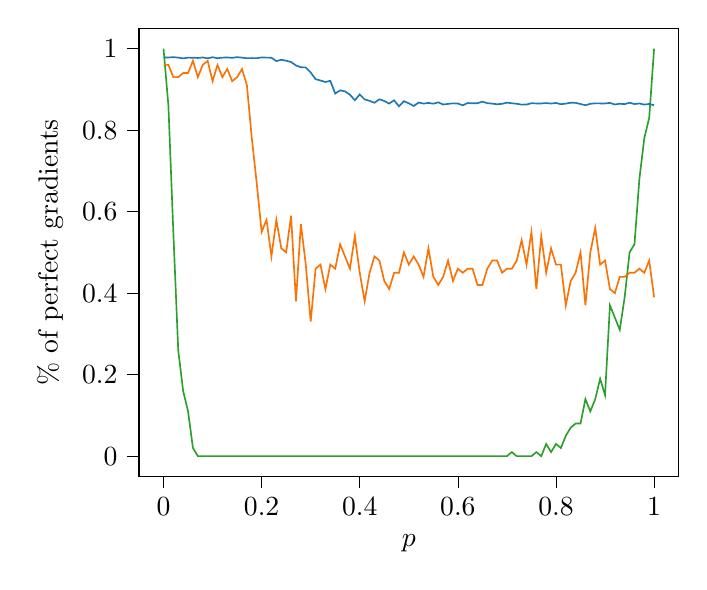
\begin{tikzpicture}

\definecolor{color0}{rgb}{0.12156862745098,0.466666666666667,0.705882352941177}
\definecolor{color1}{rgb}{0.976470588235294,0.450980392156863,0.0235294117647059}
\definecolor{color2}{rgb}{0.172549019607843,0.627450980392157,0.172549019607843}

\begin{axis}[
tick align=outside,
tick pos=left,
xlabel = $p$,
ylabel = $\%$ of perfect gradients,
x grid style={white!69.0196078431373!black},
xmin=-0.05, xmax=1.05,
xtick style={color=black},
y grid style={white!69.0196078431373!black},
ymin=-0.05, ymax=1.05,
ytick style={color=black}
]
\addplot [semithick, color2]
table {%
0 1
0.01 0.86
0.02 0.55
0.03 0.26
0.04 0.16
0.05 0.11
0.06 0.02
0.07 0
0.08 0
0.09 0
0.1 0
0.11 0
0.12 0
0.13 0
0.14 0
0.15 0
0.16 0
0.17 0
0.18 0
0.19 0
0.2 0
0.21 0
0.22 0
0.23 0
0.24 0
0.25 0
0.26 0
0.27 0
0.28 0
0.29 0
0.3 0
0.31 0
0.32 0
0.33 0
0.34 0
0.35 0
0.36 0
0.37 0
0.38 0
0.39 0
0.4 0
0.41 0
0.42 0
0.43 0
0.44 0
0.45 0
0.46 0
0.47 0
0.48 0
0.49 0
0.5 0
0.51 0
0.52 0
0.53 0
0.54 0
0.55 0
0.56 0
0.57 0
0.58 0
0.59 0
0.6 0
0.61 0
0.62 0
0.63 0
0.64 0
0.65 0
0.66 0
0.67 0
0.68 0
0.69 0
0.7 0
0.71 0.01
0.72 0
0.73 0
0.74 0
0.75 0
0.76 0.01
0.77 0
0.78 0.03
0.79 0.01
0.8 0.03
0.81 0.02
0.82 0.05
0.83 0.07
0.84 0.08
0.85 0.08
0.86 0.14
0.87 0.11
0.88 0.14
0.89 0.19
0.9 0.15
0.91 0.37
0.92 0.34
0.93 0.31
0.94 0.39
0.95 0.5
0.96 0.52
0.97 0.68
0.98 0.78
0.99 0.83
1 1
};

\addplot [semithick, color1]
table {%
0 0.96
0.01 0.96
0.02 0.93
0.03 0.93
0.04 0.94
0.05 0.94
0.06 0.97
0.07 0.93
0.08 0.96
0.09 0.97
0.1 0.92
0.11 0.96
0.12 0.93
0.13 0.95
0.14 0.92
0.15 0.93
0.16 0.95
0.17 0.91
0.18 0.78
0.19 0.67
0.2 0.55
0.21 0.58
0.22 0.49
0.23 0.58
0.24 0.51
0.25 0.5
0.26 0.59
0.27 0.38
0.28 0.57
0.29 0.47
0.3 0.33
0.31 0.46
0.32 0.47
0.33 0.41
0.34 0.47
0.35 0.46
0.36 0.52
0.37 0.49
0.38 0.46
0.39 0.54
0.4 0.45
0.41 0.38
0.42 0.45
0.43 0.49
0.44 0.48
0.45 0.43
0.46 0.41
0.47 0.45
0.48 0.45
0.49 0.5
0.5 0.47
0.51 0.49
0.52 0.47
0.53 0.44
0.54 0.51
0.55 0.44
0.56 0.42
0.57 0.44
0.58 0.48
0.59 0.43
0.6 0.46
0.61 0.45
0.62 0.46
0.63 0.46
0.64 0.42
0.65 0.42
0.66 0.46
0.67 0.48
0.68 0.48
0.69 0.45
0.7 0.46
0.71 0.46
0.72 0.48
0.73 0.53
0.74 0.47
0.75 0.55
0.76 0.41
0.77 0.54
0.78 0.45
0.79 0.51
0.8 0.47
0.81 0.47
0.82 0.37
0.83 0.43
0.84 0.45
0.85 0.5
0.86 0.37
0.87 0.5
0.88 0.56
0.89 0.47
0.9 0.48
0.91 0.41
0.92 0.4
0.93 0.44
0.94 0.44
0.95 0.45
0.96 0.45
0.97 0.46
0.98 0.45
0.99 0.48
1 0.39
};

\addplot [semithick, color0]
table {%
0 0.977919999999999
0.01 0.978279999999999
0.02 0.978919999999999
0.03 0.977939999999999
0.04 0.97596
0.05 0.977779999999999
0.06 0.977699999999999
0.07 0.977039999999999
0.08 0.97832
0.09 0.97604
0.1 0.97888
0.11 0.976419999999999
0.12 0.977859999999999
0.13 0.978259999999999
0.14 0.977419999999999
0.15 0.978939999999999
0.16 0.97788
0.17 0.97644
0.18 0.97676
0.19 0.97658
0.2 0.9783
0.21 0.977859999999999
0.22 0.97762
0.23 0.969359999999999
0.24 0.972519999999999
0.25 0.97028
0.26 0.967139999999999
0.27 0.95862
0.28 0.95432
0.29 0.953739999999999
0.3 0.9414
0.31 0.924959999999999
0.32 0.92172
0.33 0.918059999999999
0.34 0.92102
0.35 0.88968
0.36 0.897539999999999
0.37 0.89502
0.38 0.8868
0.39 0.87334
0.4 0.88752
0.41 0.87544
0.42 0.871800000000001
0.43 0.867079999999999
0.44 0.87568
0.45 0.871440000000001
0.46 0.86506
0.47 0.873139999999999
0.48 0.85838
0.49 0.87096
0.5 0.86572
0.51 0.85916
0.52 0.86772
0.53 0.86504
0.54 0.86674
0.55 0.86478
0.56 0.86816
0.57 0.86286
0.58 0.8643
0.59 0.8657
0.6 0.86518
0.61 0.860900000000001
0.62 0.86644
0.63 0.86578
0.64 0.865900000000001
0.65 0.86988
0.66 0.86608
0.67 0.864960000000001
0.68 0.86344
0.69 0.86448
0.7 0.8674
0.71 0.86586
0.72 0.86462
0.73 0.86252
0.74 0.862880000000001
0.75 0.865960000000001
0.76 0.86542
0.77 0.8654
0.78 0.8664
0.79 0.86518
0.8 0.866700000000001
0.81 0.863560000000001
0.82 0.86498
0.83 0.86728
0.84 0.86678
0.85 0.8641
0.86 0.861020000000001
0.87 0.864580000000001
0.88 0.865719999999999
0.89 0.86548
0.9 0.86548
0.91 0.866820000000001
0.92 0.86288
0.93 0.864700000000001
0.94 0.86376
0.95 0.867220000000001
0.96 0.86396
0.97 0.865320000000001
0.98 0.8626
0.99 0.86418
1 0.861
};
\end{axis}

\end{tikzpicture}

\end{center}
\end{subfigure}
\caption{How often do apparent gradients of  $Y_2(15,p)$ yield perfect Morse matchings (green) compared to how often the random discrete Morse function yields perfect Morse matchings for $Y_2(10,p)$ (blue) and $Y_2(15,p)$ (orange).}
\label{fig:perfect_rdm_v_apparent}
\end{figure}

Figure \ref{fig:perfect_rdm_v_apparent} allows two interesting observations. Firstly in terms of the apparent gradients, we see the same behaviour for $Y_2(15,p)$ as for $Y_2(10,p)$, although for $Y_2(15,p)$, the initial decline is steeper and the percentage of perfect apparent gradients also starts to rise again later. Indeed for any $p \notin \{0,1\}$ and $n$ large enough we expect there to be at least one configuration in the filtration where some simplex can not get paired with respect to apparent pairs. Hence the apparent gradient is not perfect. Therefore the larger the value for $n$ the lower the value of $p$ for which we might get a perfect apparent gradient. A similar argument explains the behavior for values of $p$ close to $1$. This means that for $n \rightarrow \infty$ we get perfect gradients if and only if $p \in \{0,1\}$.

Secondly we see that initially the random discrete Morse algorithm has a very high probability of finding a perfect Morse matching for $Y_2(10,p)$ and $Y_2(15,p)$. Then we get a  decline at around $p = 0.25$ and $p = 0.19$ respectively. Afterwards fewer of the found Morse matchings are perfect. It is surprising to see these different levels for different $n$ which seem to be quite stable over large ranges of values for $p$. 

In some future work we would like to find some explanation for this sudden jump in the percentage of perfect Morse matchings found by the random discrete Morse algorithm. The following figure could give a potential clue or starting point for further exploration. It shows a plot of the sum of Betti numbers of random $2$-complexes averaged over $50$ runs.

\begin{figure}[H]
%\centering%
\begin{subfigure}[c]{0.95\textwidth}
\begin{center}
% This file was created by tikzplotlib v0.9.2.
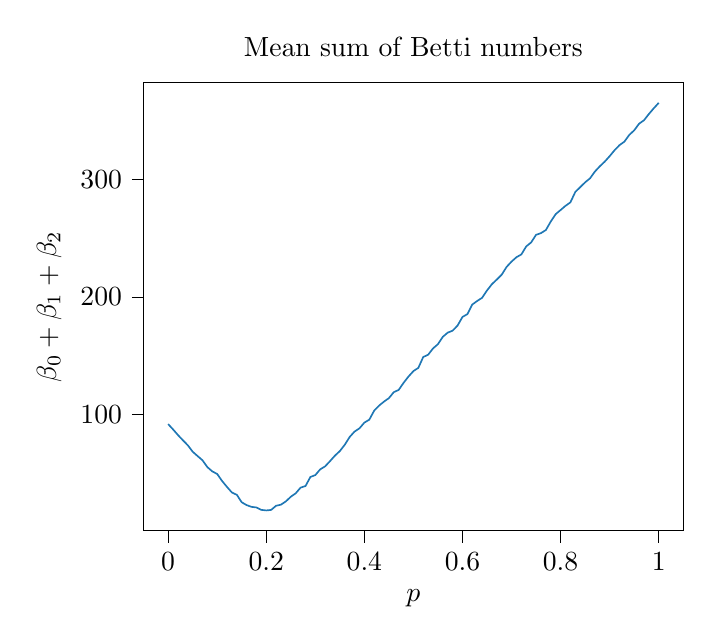
\begin{tikzpicture}

\definecolor{color0}{rgb}{0.12156862745098,0.466666666666667,0.705882352941177}

\begin{axis}[
tick align=outside,
tick pos=left,
title={Mean sum of Betti numbers},
xlabel = $p$,
ylabel = $\beta_0 + \beta_1 + \beta_2$,
x grid style={white!69.0196078431373!black},
xmin=-0.05, xmax=1.05,
xtick style={color=black},
y grid style={white!69.0196078431373!black},
ymin=1.301, ymax=382.319,
ytick style={color=black}
]
\addplot [semithick, color0]
table {%
0 92
0.01 87.5
0.02 82.72
0.03 78.3
0.04 74.06
0.05 68.54
0.06 64.86
0.07 61.26
0.08 55.44
0.09 51.8
0.1 49.62
0.11 43.64
0.12 38.6
0.13 33.86
0.14 31.9
0.15 25.56
0.16 23.14
0.17 21.64
0.18 21.16
0.19 19.1
0.2 18.62
0.21 19.06
0.22 22.6
0.23 23.5
0.24 26.3
0.25 30.24
0.26 33.16
0.27 38
0.28 39.34
0.29 47.06
0.3 48.66
0.31 53.54
0.32 56.08
0.33 60.5
0.34 65.18
0.35 69.06
0.36 74.4
0.37 81.02
0.38 85.66
0.39 88.38
0.4 93.26
0.41 95.72
0.42 103.42
0.43 107.72
0.44 111.1
0.45 114.06
0.46 119.14
0.47 121.06
0.48 127.1
0.49 132.44
0.5 137.02
0.51 139.78
0.52 149.02
0.53 150.94
0.54 156.3
0.55 159.94
0.56 166.2
0.57 169.74
0.58 171.42
0.59 175.76
0.6 183.06
0.61 185.46
0.62 193.62
0.63 196.64
0.64 199.34
0.65 205.56
0.66 210.92
0.67 214.86
0.68 219
0.69 225.62
0.7 230.1
0.71 233.82
0.72 236.18
0.73 243.04
0.74 246.4
0.75 252.88
0.76 254.3
0.77 256.94
0.78 264.16
0.79 270.44
0.8 273.94
0.81 277.48
0.82 280.46
0.83 289.3
0.84 293.36
0.85 297.48
0.86 300.86
0.87 306.66
0.88 311.12
0.89 315.08
0.9 319.7
0.91 324.74
0.92 329.04
0.93 332.04
0.94 337.78
0.95 341.66
0.96 347.28
0.97 350.24
0.98 355.56
0.99 360.44
1 365
};
\end{axis}

\end{tikzpicture}

\end{center}
\end{subfigure}
\caption{Sum of Betti numbers for $Y_2(15,p)$.}
\label{fig:summed_bettis}
\end{figure}

As we can see the sum of Betti numbers declines until $p$ reaches a value of about $0.2$ which is close to the value at which we see a jump in the percentage of perfect Morse matchings found by the random discrete Morse function. 

If in some practical situation one is interested in a perfect Morse matching on a random $k$-complex, in most cases searching for one via the random discrete Morse algorithm is the better way to go. For very small and very large values of $p$ however it might be a good idea to check the apparent gradient. 

\section{Alpha Complexes on Random Point Clouds}

Recall the definition of alpha complexes from Section \ref{sec:filtrations_from_point_clouds}. The set of points we construct the complex on can have a variety of origins. Maybe it is real world data of some kind or a handpicked set of points or, as in our case, some randomly generated set of points. By randomly generated we mean that each point is sampled via some random distribution. 

We generate point clouds using the \textbf{numpy.random} library for \textbf{Python3}, then we calculate the (inclusion-wise) largest possible Alpha complex on the point cloud and a simplexwise filtration of it using the \textbf{GUDHI} library. The exact construction is specified in \cite{gudhi_alpha}.

We chose the following distributions, since they also appear in real world situations. 

\subsection{Uniform Distribution}
In this case, we will sample from the $k$-dimensional unit cube.
For a point $p = (p_1, \dots, p_k)$ this means that each $p_i$ is drawn from the interval $[0,1]$ and that each value in the interval is equally likely. In other words the probability density we draw from equals one on the $k$-dimensional unit cube and zero elsewhere. Figure \ref{fig:uniform} gives an example of a two dimensional point cloud consisting of 100 points drawn like this. Subfigure (b) shows the simplicial complex $K_{\lfloor \frac{n}{2}\rfloor}$ of the filtration $F_* = \{K_1,\dots,K_n\}$, where $K_n$ is the Alpha complex, where $\epsilon > 0$ is so large, that further increasing its value does not change the resulting simplicial complex, which we will call the \textbf{maximal alpha complex}. 

Due to the discrete nature of floating point precision it is possible, although very unlikely, that several simplices appear at the same distance $\epsilon$. In this case we sort the simplices by dimension first and lexicographically second, hence we always get a simplexwise filtration.

\begin{figure}[H]
%\centering%
\begin{subfigure}[t]{0.49\textwidth}
\begin{center}
% This file was created by tikzplotlib v0.9.2.
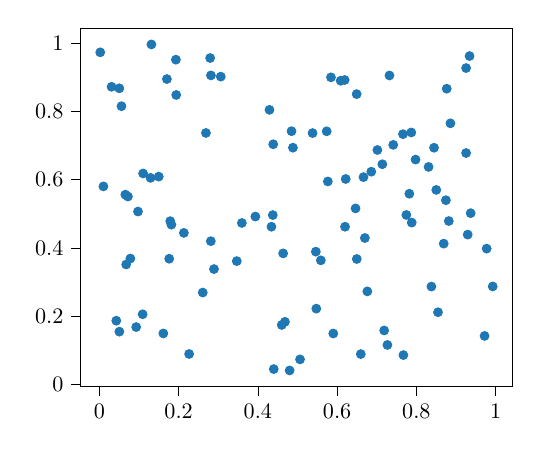
\begin{tikzpicture}[thick,scale=0.8, every node/.style={transform shape}]

\definecolor{color0}{rgb}{0.12156862745098,0.466666666666667,0.705882352941177}

\begin{axis}[
tick align=outside,
tick pos=left,
x grid style={white!69.0196078431373!black},
xmin=-0.0472016021677426, xmax=1.04212434473219,
xtick style={color=black},
y grid style={white!69.0196078431373!black},
ymin=-0.00675939644529908, ymax=1.04406901760383,
ytick style={color=black}
]
\addplot [only marks, mark=*, draw=color0, fill=color0, colormap/viridis]
table{%
x                      y
0.0656955078449548 0.556158704850788
0.488517157678954 0.69370505416162
0.181862561225007 0.468128175467136
0.844533344061402 0.693545891548072
0.437740280960978 0.496309026394877
0.767231562363555 0.0860675211731177
0.161530883369563 0.149522611184683
0.788251177639878 0.474286327772315
0.766192297835678 0.733348483357132
0.649617451878118 0.367644291551499
0.0504928809316121 0.867642915553829
0.170496234193967 0.894845379322294
0.718729700185543 0.158201872935623
0.463819403422516 0.384045617799055
0.546308284855135 0.389105087054855
0.850219712772608 0.569999593186233
0.0428039347057998 0.18679851387532
0.573667306869477 0.74169251615805
0.830796451137699 0.637386850693855
0.09754863385918 0.506639045306481
0.176293594034698 0.368347919534268
0.558945574150558 0.363726295676814
0.787179566858828 0.738324537463096
0.732125010276887 0.905322560907993
0.440152466660368 0.0450691086687682
0.874505181504566 0.539834503981332
0.359650163755757 0.473142318396389
0.88183940202602 0.47882764457561
0.6190674997885 0.892085167037166
0.620007468347855 0.462139938538465
0.434312621954214 0.462123559134768
0.0558809818709056 0.815333816765134
0.460296317457924 0.174337725374721
0.937004669450955 0.501883644124649
0.129208296418927 0.60524715222521
0.621711178101921 0.602058371214988
0.0930339583508482 0.168174189826023
0.646497637212577 0.515829619327083
0.00231321360043601 0.973121363384185
0.269010530488123 0.736864398451098
0.67623642837757 0.272719320218006
0.48499005939712 0.742084656413199
0.468336897848343 0.183551404784195
0.741566295886979 0.701998568075081
0.226614592948441 0.0892462234244782
0.854492515665868 0.211588735873265
0.0103020564667987 0.580327888091732
0.70164552814407 0.687005996723676
0.306448355159162 0.901946766882589
0.6665798023091 0.60748307490518
0.649320898379969 0.850722397546172
0.429368424142197 0.804574630420432
0.576602731405145 0.594803970012622
0.48015110475138 0.0410055314660248
0.346814709956971 0.361390601145233
0.669995242191944 0.429101602778892
0.0308665950142099 0.872116233796655
0.0505858065112469 0.15467441279092
0.281620589189466 0.905552902924876
0.547524146840316 0.222137875364193
0.972105186204234 0.142213802563758
0.797951124554537 0.658900075698976
0.281347270295641 0.419788547388917
0.584518692663292 0.899839075148078
0.506434656037461 0.0734659500132817
0.686220186190104 0.623421790253092
0.934165564467276 0.962202483589049
0.131454879873151 0.996304089692503
0.885904610919406 0.765107958160786
0.28931761684864 0.338033790105762
0.876577875921493 0.866575669683953
0.193206840334259 0.951591205744689
0.925478745500447 0.9270343379018
0.726874021864532 0.115775075441666
0.782219352465157 0.558773137671638
0.868971829466657 0.412584348571824
0.977330218354481 0.397931727754565
0.714167369203424 0.645271412265081
0.213331794086431 0.444102592245728
0.279648133171411 0.956420011538135
0.0721688416845659 0.550630971981264
0.260963862668663 0.269311361195102
0.590350068616808 0.149312398274075
0.608963404612232 0.889896844048345
0.149963024059017 0.608943668591563
0.992609528964008 0.287200579008376
0.774734133265123 0.496627215016348
0.929472829761068 0.439095720490705
0.110434792844883 0.618239477228263
0.109298875857005 0.205648545579206
0.393767944012354 0.491990742021887
0.0783566045417764 0.369000302058699
0.659726956866604 0.0889856647168015
0.438741749568941 0.703747806517045
0.538058398480968 0.736545720828899
0.837906975806817 0.286819511659124
0.179003186619879 0.478469594552395
0.925475163513836 0.67809841245703
0.194055592803374 0.848205002543498
0.0677117661935651 0.351520919888751
};
\end{axis}

\end{tikzpicture}

\subcaption{Point cloud $S$}
\end{center}
\end{subfigure}
\begin{subfigure}[t]{0.49\textwidth}
\begin{center}
% This file was created by tikzplotlib v0.9.2.
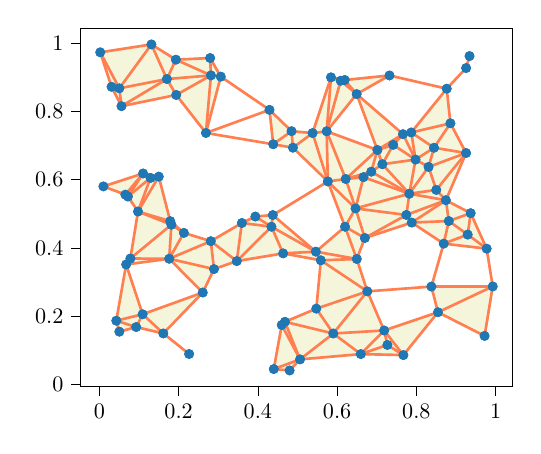
\begin{tikzpicture}[thick,scale=0.8, every node/.style={transform shape}]

\definecolor{color0}{rgb}{0.12156862745098,0.466666666666667,0.705882352941177}
\definecolor{color1}{rgb}{1,0.498039215686275,0.0549019607843137}
\definecolor{color2}{rgb}{0.96078431372549,0.96078431372549,0.862745098039216}
\definecolor{color3}{rgb}{1,0.498039215686275,0.313725490196078}

\begin{axis}[
tick align=outside,
tick pos=left,
x grid style={white!69.0196078431373!black},
xmin=-0.0472016021677426, xmax=1.04212434473219,
xtick style={color=black},
y grid style={white!69.0196078431373!black},
ymin=-0.0067593964452991, ymax=1.04406901760383,
ytick style={color=black}
]
\addplot [only marks, mark=*, draw=color0, fill=color0, colormap/viridis]
table{%
x                      y
0.0656955078449548 0.556158704850788
0.488517157678954 0.69370505416162
0.181862561225007 0.468128175467136
0.844533344061402 0.693545891548072
0.437740280960978 0.496309026394877
0.767231562363555 0.0860675211731177
0.161530883369563 0.149522611184683
0.788251177639878 0.474286327772315
0.766192297835678 0.733348483357132
0.649617451878118 0.367644291551499
0.0504928809316121 0.867642915553829
0.170496234193967 0.894845379322294
0.718729700185543 0.158201872935623
0.463819403422516 0.384045617799055
0.546308284855135 0.389105087054855
0.850219712772608 0.569999593186233
0.0428039347057998 0.18679851387532
0.573667306869477 0.74169251615805
0.830796451137699 0.637386850693855
0.09754863385918 0.506639045306481
0.176293594034698 0.368347919534268
0.558945574150558 0.363726295676814
0.787179566858828 0.738324537463096
0.732125010276887 0.905322560907993
0.440152466660368 0.0450691086687682
0.874505181504566 0.539834503981332
0.359650163755757 0.473142318396389
0.88183940202602 0.47882764457561
0.6190674997885 0.892085167037166
0.620007468347855 0.462139938538465
0.434312621954214 0.462123559134768
0.0558809818709056 0.815333816765134
0.460296317457924 0.174337725374721
0.937004669450955 0.501883644124649
0.129208296418927 0.60524715222521
0.621711178101921 0.602058371214988
0.0930339583508482 0.168174189826023
0.646497637212577 0.515829619327083
0.00231321360043601 0.973121363384185
0.269010530488123 0.736864398451098
0.67623642837757 0.272719320218006
0.48499005939712 0.742084656413199
0.468336897848343 0.183551404784195
0.741566295886979 0.701998568075081
0.226614592948441 0.0892462234244782
0.854492515665868 0.211588735873265
0.0103020564667987 0.580327888091732
0.70164552814407 0.687005996723676
0.306448355159162 0.901946766882589
0.6665798023091 0.60748307490518
0.649320898379969 0.850722397546172
0.429368424142197 0.804574630420432
0.576602731405145 0.594803970012622
0.48015110475138 0.0410055314660248
0.346814709956971 0.361390601145233
0.669995242191944 0.429101602778892
0.0308665950142099 0.872116233796655
0.0505858065112469 0.15467441279092
0.281620589189466 0.905552902924876
0.547524146840316 0.222137875364193
0.972105186204234 0.142213802563758
0.797951124554537 0.658900075698976
0.281347270295641 0.419788547388917
0.584518692663292 0.899839075148078
0.506434656037461 0.0734659500132817
0.686220186190104 0.623421790253092
0.934165564467276 0.962202483589049
0.131454879873151 0.996304089692503
0.885904610919406 0.765107958160786
0.28931761684864 0.338033790105762
0.876577875921493 0.866575669683953
0.193206840334259 0.951591205744689
0.925478745500447 0.9270343379018
0.726874021864532 0.115775075441666
0.782219352465157 0.558773137671638
0.868971829466657 0.412584348571824
0.977330218354481 0.397931727754565
0.714167369203424 0.645271412265081
0.213331794086431 0.444102592245728
0.279648133171411 0.956420011538135
0.0721688416845659 0.550630971981264
0.260963862668663 0.269311361195102
0.590350068616808 0.149312398274075
0.608963404612232 0.889896844048345
0.149963024059017 0.608943668591563
0.992609528964008 0.287200579008376
0.774734133265123 0.496627215016348
0.929472829761068 0.439095720490705
0.110434792844883 0.618239477228263
0.109298875857005 0.205648545579206
0.393767944012354 0.491990742021887
0.0783566045417764 0.369000302058699
0.659726956866604 0.0889856647168015
0.438741749568941 0.703747806517045
0.538058398480968 0.736545720828899
0.837906975806817 0.286819511659124
0.179003186619879 0.478469594552395
0.925475163513836 0.67809841245703
0.194055592803374 0.848205002543498
0.0677117661935651 0.351520919888751
};
\path [draw=color2, fill=color2]
(axis cs:0.437740280960978,0.496309026394877)
--(axis cs:0.434312621954214,0.462123559134768)
--(axis cs:0.393767944012354,0.491990742021887)
--cycle;
\path [draw=color2, fill=color2]
(axis cs:0.0428039347057998,0.18679851387532)
--(axis cs:0.0930339583508482,0.168174189826023)
--(axis cs:0.0505858065112469,0.15467441279092)
--cycle;
\path [draw=color2, fill=color2]
(axis cs:0.129208296418927,0.60524715222521)
--(axis cs:0.149963024059017,0.608943668591563)
--(axis cs:0.110434792844883,0.618239477228263)
--cycle;
\path [draw=color2, fill=color2]
(axis cs:0.6190674997885,0.892085167037166)
--(axis cs:0.649320898379969,0.850722397546172)
--(axis cs:0.608963404612232,0.889896844048345)
--cycle;
\path [draw=color2, fill=color2]
(axis cs:0.844533344061402,0.693545891548072)
--(axis cs:0.830796451137699,0.637386850693855)
--(axis cs:0.797951124554537,0.658900075698976)
--cycle;
\path [draw=color2, fill=color2]
(axis cs:0.306448355159162,0.901946766882589)
--(axis cs:0.281620589189466,0.905552902924876)
--(axis cs:0.279648133171411,0.956420011538135)
--cycle;
\path [draw=color2, fill=color2]
(axis cs:0.488517157678954,0.69370505416162)
--(axis cs:0.48499005939712,0.742084656413199)
--(axis cs:0.438741749568941,0.703747806517045)
--cycle;
\path [draw=color2, fill=color2]
(axis cs:0.6190674997885,0.892085167037166)
--(axis cs:0.584518692663292,0.899839075148078)
--(axis cs:0.608963404612232,0.889896844048345)
--cycle;
\path [draw=color2, fill=color2]
(axis cs:0.741566295886979,0.701998568075081)
--(axis cs:0.70164552814407,0.687005996723676)
--(axis cs:0.714167369203424,0.645271412265081)
--cycle;
\path [draw=color2, fill=color2]
(axis cs:0.0504928809316121,0.867642915553829)
--(axis cs:0.0558809818709056,0.815333816765134)
--(axis cs:0.0308665950142099,0.872116233796655)
--cycle;
\path [draw=color2, fill=color2]
(axis cs:0.488517157678954,0.69370505416162)
--(axis cs:0.48499005939712,0.742084656413199)
--(axis cs:0.538058398480968,0.736545720828899)
--cycle;
\path [draw=color2, fill=color2]
(axis cs:0.0428039347057998,0.18679851387532)
--(axis cs:0.0930339583508482,0.168174189826023)
--(axis cs:0.109298875857005,0.205648545579206)
--cycle;
\path [draw=color2, fill=color2]
(axis cs:0.70164552814407,0.687005996723676)
--(axis cs:0.686220186190104,0.623421790253092)
--(axis cs:0.714167369203424,0.645271412265081)
--cycle;
\path [draw=color2, fill=color2]
(axis cs:0.88183940202602,0.47882764457561)
--(axis cs:0.937004669450955,0.501883644124649)
--(axis cs:0.929472829761068,0.439095720490705)
--cycle;
\path [draw=color2, fill=color2]
(axis cs:0.88183940202602,0.47882764457561)
--(axis cs:0.868971829466657,0.412584348571824)
--(axis cs:0.929472829761068,0.439095720490705)
--cycle;
\path [draw=color2, fill=color2]
(axis cs:0.874505181504566,0.539834503981332)
--(axis cs:0.88183940202602,0.47882764457561)
--(axis cs:0.937004669450955,0.501883644124649)
--cycle;
\path [draw=color2, fill=color2]
(axis cs:0.161530883369563,0.149522611184683)
--(axis cs:0.0930339583508482,0.168174189826023)
--(axis cs:0.109298875857005,0.205648545579206)
--cycle;
\path [draw=color2, fill=color2]
(axis cs:0.0656955078449548,0.556158704850788)
--(axis cs:0.0721688416845659,0.550630971981264)
--(axis cs:0.110434792844883,0.618239477228263)
--cycle;
\path [draw=color2, fill=color2]
(axis cs:0.129208296418927,0.60524715222521)
--(axis cs:0.0721688416845659,0.550630971981264)
--(axis cs:0.110434792844883,0.618239477228263)
--cycle;
\path [draw=color2, fill=color2]
(axis cs:0.181862561225007,0.468128175467136)
--(axis cs:0.213331794086431,0.444102592245728)
--(axis cs:0.179003186619879,0.478469594552395)
--cycle;
\path [draw=color2, fill=color2]
(axis cs:0.766192297835678,0.733348483357132)
--(axis cs:0.741566295886979,0.701998568075081)
--(axis cs:0.797951124554537,0.658900075698976)
--cycle;
\path [draw=color2, fill=color2]
(axis cs:0.766192297835678,0.733348483357132)
--(axis cs:0.787179566858828,0.738324537463096)
--(axis cs:0.797951124554537,0.658900075698976)
--cycle;
\path [draw=color2, fill=color2]
(axis cs:0.359650163755757,0.473142318396389)
--(axis cs:0.434312621954214,0.462123559134768)
--(axis cs:0.393767944012354,0.491990742021887)
--cycle;
\path [draw=color2, fill=color2]
(axis cs:0.844533344061402,0.693545891548072)
--(axis cs:0.787179566858828,0.738324537463096)
--(axis cs:0.797951124554537,0.658900075698976)
--cycle;
\path [draw=color2, fill=color2]
(axis cs:0.440152466660368,0.0450691086687682)
--(axis cs:0.48015110475138,0.0410055314660248)
--(axis cs:0.506434656037461,0.0734659500132817)
--cycle;
\path [draw=color2, fill=color2]
(axis cs:0.741566295886979,0.701998568075081)
--(axis cs:0.797951124554537,0.658900075698976)
--(axis cs:0.714167369203424,0.645271412265081)
--cycle;
\path [draw=color2, fill=color2]
(axis cs:0.620007468347855,0.462139938538465)
--(axis cs:0.646497637212577,0.515829619327083)
--(axis cs:0.669995242191944,0.429101602778892)
--cycle;
\path [draw=color2, fill=color2]
(axis cs:0.346814709956971,0.361390601145233)
--(axis cs:0.281347270295641,0.419788547388917)
--(axis cs:0.28931761684864,0.338033790105762)
--cycle;
\path [draw=color2, fill=color2]
(axis cs:0.718729700185543,0.158201872935623)
--(axis cs:0.726874021864532,0.115775075441666)
--(axis cs:0.659726956866604,0.0889856647168015)
--cycle;
\path [draw=color2, fill=color2]
(axis cs:0.850219712772608,0.569999593186233)
--(axis cs:0.830796451137699,0.637386850693855)
--(axis cs:0.782219352465157,0.558773137671638)
--cycle;
\path [draw=color2, fill=color2]
(axis cs:0.621711178101921,0.602058371214988)
--(axis cs:0.646497637212577,0.515829619327083)
--(axis cs:0.6665798023091,0.60748307490518)
--cycle;
\path [draw=color2, fill=color2]
(axis cs:0.281620589189466,0.905552902924876)
--(axis cs:0.193206840334259,0.951591205744689)
--(axis cs:0.279648133171411,0.956420011538135)
--cycle;
\path [draw=color2, fill=color2]
(axis cs:0.844533344061402,0.693545891548072)
--(axis cs:0.885904610919406,0.765107958160786)
--(axis cs:0.925475163513836,0.67809841245703)
--cycle;
\path [draw=color2, fill=color2]
(axis cs:0.48499005939712,0.742084656413199)
--(axis cs:0.429368424142197,0.804574630420432)
--(axis cs:0.438741749568941,0.703747806517045)
--cycle;
\path [draw=color2, fill=color2]
(axis cs:0.830796451137699,0.637386850693855)
--(axis cs:0.797951124554537,0.658900075698976)
--(axis cs:0.782219352465157,0.558773137671638)
--cycle;
\path [draw=color2, fill=color2]
(axis cs:0.181862561225007,0.468128175467136)
--(axis cs:0.176293594034698,0.368347919534268)
--(axis cs:0.213331794086431,0.444102592245728)
--cycle;
\path [draw=color2, fill=color2]
(axis cs:0.649617451878118,0.367644291551499)
--(axis cs:0.620007468347855,0.462139938538465)
--(axis cs:0.669995242191944,0.429101602778892)
--cycle;
\path [draw=color2, fill=color2]
(axis cs:0.844533344061402,0.693545891548072)
--(axis cs:0.830796451137699,0.637386850693855)
--(axis cs:0.925475163513836,0.67809841245703)
--cycle;
\path [draw=color2, fill=color2]
(axis cs:0.844533344061402,0.693545891548072)
--(axis cs:0.787179566858828,0.738324537463096)
--(axis cs:0.885904610919406,0.765107958160786)
--cycle;
\path [draw=color2, fill=color2]
(axis cs:0.788251177639878,0.474286327772315)
--(axis cs:0.88183940202602,0.47882764457561)
--(axis cs:0.868971829466657,0.412584348571824)
--cycle;
\path [draw=color2, fill=color2]
(axis cs:0.463819403422516,0.384045617799055)
--(axis cs:0.546308284855135,0.389105087054855)
--(axis cs:0.558945574150558,0.363726295676814)
--cycle;
\path [draw=color2, fill=color2]
(axis cs:0.621711178101921,0.602058371214988)
--(axis cs:0.646497637212577,0.515829619327083)
--(axis cs:0.576602731405145,0.594803970012622)
--cycle;
\path [draw=color2, fill=color2]
(axis cs:0.09754863385918,0.506639045306481)
--(axis cs:0.129208296418927,0.60524715222521)
--(axis cs:0.0721688416845659,0.550630971981264)
--cycle;
\path [draw=color2, fill=color2]
(axis cs:0.850219712772608,0.569999593186233)
--(axis cs:0.874505181504566,0.539834503981332)
--(axis cs:0.782219352465157,0.558773137671638)
--cycle;
\path [draw=color2, fill=color2]
(axis cs:0.788251177639878,0.474286327772315)
--(axis cs:0.874505181504566,0.539834503981332)
--(axis cs:0.88183940202602,0.47882764457561)
--cycle;
\path [draw=color2, fill=color2]
(axis cs:0.874505181504566,0.539834503981332)
--(axis cs:0.782219352465157,0.558773137671638)
--(axis cs:0.774734133265123,0.496627215016348)
--cycle;
\path [draw=color2, fill=color2]
(axis cs:0.788251177639878,0.474286327772315)
--(axis cs:0.874505181504566,0.539834503981332)
--(axis cs:0.774734133265123,0.496627215016348)
--cycle;
\path [draw=color2, fill=color2]
(axis cs:0.0656955078449548,0.556158704850788)
--(axis cs:0.0103020564667987,0.580327888091732)
--(axis cs:0.110434792844883,0.618239477228263)
--cycle;
\path [draw=color2, fill=color2]
(axis cs:0.170496234193967,0.894845379322294)
--(axis cs:0.131454879873151,0.996304089692503)
--(axis cs:0.193206840334259,0.951591205744689)
--cycle;
\path [draw=color2, fill=color2]
(axis cs:0.170496234193967,0.894845379322294)
--(axis cs:0.281620589189466,0.905552902924876)
--(axis cs:0.193206840334259,0.951591205744689)
--cycle;
\path [draw=color2, fill=color2]
(axis cs:0.170496234193967,0.894845379322294)
--(axis cs:0.281620589189466,0.905552902924876)
--(axis cs:0.194055592803374,0.848205002543498)
--cycle;
\path [draw=color2, fill=color2]
(axis cs:0.181862561225007,0.468128175467136)
--(axis cs:0.09754863385918,0.506639045306481)
--(axis cs:0.179003186619879,0.478469594552395)
--cycle;
\path [draw=color2, fill=color2]
(axis cs:0.732125010276887,0.905322560907993)
--(axis cs:0.6190674997885,0.892085167037166)
--(axis cs:0.649320898379969,0.850722397546172)
--cycle;
\path [draw=color2, fill=color2]
(axis cs:0.649617451878118,0.367644291551499)
--(axis cs:0.546308284855135,0.389105087054855)
--(axis cs:0.558945574150558,0.363726295676814)
--cycle;
\path [draw=color2, fill=color2]
(axis cs:0.686220186190104,0.623421790253092)
--(axis cs:0.782219352465157,0.558773137671638)
--(axis cs:0.714167369203424,0.645271412265081)
--cycle;
\path [draw=color2, fill=color2]
(axis cs:0.797951124554537,0.658900075698976)
--(axis cs:0.782219352465157,0.558773137671638)
--(axis cs:0.714167369203424,0.645271412265081)
--cycle;
\path [draw=color2, fill=color2]
(axis cs:0.359650163755757,0.473142318396389)
--(axis cs:0.346814709956971,0.361390601145233)
--(axis cs:0.281347270295641,0.419788547388917)
--cycle;
\path [draw=color2, fill=color2]
(axis cs:0.176293594034698,0.368347919534268)
--(axis cs:0.281347270295641,0.419788547388917)
--(axis cs:0.213331794086431,0.444102592245728)
--cycle;
\path [draw=color2, fill=color2]
(axis cs:0.649617451878118,0.367644291551499)
--(axis cs:0.546308284855135,0.389105087054855)
--(axis cs:0.620007468347855,0.462139938538465)
--cycle;
\path [draw=color2, fill=color2]
(axis cs:0.868971829466657,0.412584348571824)
--(axis cs:0.977330218354481,0.397931727754565)
--(axis cs:0.929472829761068,0.439095720490705)
--cycle;
\path [draw=color2, fill=color2]
(axis cs:0.176293594034698,0.368347919534268)
--(axis cs:0.281347270295641,0.419788547388917)
--(axis cs:0.28931761684864,0.338033790105762)
--cycle;
\path [draw=color2, fill=color2]
(axis cs:0.788251177639878,0.474286327772315)
--(axis cs:0.669995242191944,0.429101602778892)
--(axis cs:0.774734133265123,0.496627215016348)
--cycle;
\path [draw=color2, fill=color2]
(axis cs:0.767231562363555,0.0860675211731177)
--(axis cs:0.726874021864532,0.115775075441666)
--(axis cs:0.659726956866604,0.0889856647168015)
--cycle;
\path [draw=color2, fill=color2]
(axis cs:0.468336897848343,0.183551404784195)
--(axis cs:0.547524146840316,0.222137875364193)
--(axis cs:0.590350068616808,0.149312398274075)
--cycle;
\path [draw=color2, fill=color2]
(axis cs:0.621711178101921,0.602058371214988)
--(axis cs:0.6665798023091,0.60748307490518)
--(axis cs:0.686220186190104,0.623421790253092)
--cycle;
\path [draw=color2, fill=color2]
(axis cs:0.460296317457924,0.174337725374721)
--(axis cs:0.468336897848343,0.183551404784195)
--(axis cs:0.506434656037461,0.0734659500132817)
--cycle;
\path [draw=color2, fill=color2]
(axis cs:0.767231562363555,0.0860675211731177)
--(axis cs:0.718729700185543,0.158201872935623)
--(axis cs:0.726874021864532,0.115775075441666)
--cycle;
\path [draw=color2, fill=color2]
(axis cs:0.176293594034698,0.368347919534268)
--(axis cs:0.0783566045417764,0.369000302058699)
--(axis cs:0.0677117661935651,0.351520919888751)
--cycle;
\path [draw=color2, fill=color2]
(axis cs:0.718729700185543,0.158201872935623)
--(axis cs:0.590350068616808,0.149312398274075)
--(axis cs:0.659726956866604,0.0889856647168015)
--cycle;
\path [draw=color2, fill=color2]
(axis cs:0.09754863385918,0.506639045306481)
--(axis cs:0.129208296418927,0.60524715222521)
--(axis cs:0.149963024059017,0.608943668591563)
--cycle;
\path [draw=color2, fill=color2]
(axis cs:0.440152466660368,0.0450691086687682)
--(axis cs:0.460296317457924,0.174337725374721)
--(axis cs:0.506434656037461,0.0734659500132817)
--cycle;
\path [draw=color2, fill=color2]
(axis cs:0.6665798023091,0.60748307490518)
--(axis cs:0.686220186190104,0.623421790253092)
--(axis cs:0.782219352465157,0.558773137671638)
--cycle;
\path [draw=color2, fill=color2]
(axis cs:0.176293594034698,0.368347919534268)
--(axis cs:0.28931761684864,0.338033790105762)
--(axis cs:0.260963862668663,0.269311361195102)
--cycle;
\path [draw=color2, fill=color2]
(axis cs:0.0504928809316121,0.867642915553829)
--(axis cs:0.00231321360043601,0.973121363384185)
--(axis cs:0.0308665950142099,0.872116233796655)
--cycle;
\path [draw=color2, fill=color2]
(axis cs:0.850219712772608,0.569999593186233)
--(axis cs:0.830796451137699,0.637386850693855)
--(axis cs:0.925475163513836,0.67809841245703)
--cycle;
\path [draw=color2, fill=color2]
(axis cs:0.359650163755757,0.473142318396389)
--(axis cs:0.434312621954214,0.462123559134768)
--(axis cs:0.346814709956971,0.361390601145233)
--cycle;
\path [draw=color2, fill=color2]
(axis cs:0.937004669450955,0.501883644124649)
--(axis cs:0.977330218354481,0.397931727754565)
--(axis cs:0.929472829761068,0.439095720490705)
--cycle;
\path [draw=color2, fill=color2]
(axis cs:0.09754863385918,0.506639045306481)
--(axis cs:0.149963024059017,0.608943668591563)
--(axis cs:0.179003186619879,0.478469594552395)
--cycle;
\path [draw=color2, fill=color2]
(axis cs:0.463819403422516,0.384045617799055)
--(axis cs:0.434312621954214,0.462123559134768)
--(axis cs:0.346814709956971,0.361390601145233)
--cycle;
\path [draw=color2, fill=color2]
(axis cs:0.646497637212577,0.515829619327083)
--(axis cs:0.669995242191944,0.429101602778892)
--(axis cs:0.774734133265123,0.496627215016348)
--cycle;
\path [draw=color2, fill=color2]
(axis cs:0.621711178101921,0.602058371214988)
--(axis cs:0.70164552814407,0.687005996723676)
--(axis cs:0.686220186190104,0.623421790253092)
--cycle;
\path [draw=color2, fill=color2]
(axis cs:0.468336897848343,0.183551404784195)
--(axis cs:0.506434656037461,0.0734659500132817)
--(axis cs:0.590350068616808,0.149312398274075)
--cycle;
\path [draw=color2, fill=color2]
(axis cs:0.463819403422516,0.384045617799055)
--(axis cs:0.546308284855135,0.389105087054855)
--(axis cs:0.434312621954214,0.462123559134768)
--cycle;
\path [draw=color2, fill=color2]
(axis cs:0.0504928809316121,0.867642915553829)
--(axis cs:0.170496234193967,0.894845379322294)
--(axis cs:0.0558809818709056,0.815333816765134)
--cycle;
\path [draw=color2, fill=color2]
(axis cs:0.646497637212577,0.515829619327083)
--(axis cs:0.782219352465157,0.558773137671638)
--(axis cs:0.774734133265123,0.496627215016348)
--cycle;
\path [draw=color2, fill=color2]
(axis cs:0.170496234193967,0.894845379322294)
--(axis cs:0.0558809818709056,0.815333816765134)
--(axis cs:0.194055592803374,0.848205002543498)
--cycle;
\path [draw=color2, fill=color2]
(axis cs:0.181862561225007,0.468128175467136)
--(axis cs:0.176293594034698,0.368347919534268)
--(axis cs:0.0783566045417764,0.369000302058699)
--cycle;
\path [draw=color2, fill=color2]
(axis cs:0.646497637212577,0.515829619327083)
--(axis cs:0.6665798023091,0.60748307490518)
--(axis cs:0.782219352465157,0.558773137671638)
--cycle;
\path [draw=color2, fill=color2]
(axis cs:0.488517157678954,0.69370505416162)
--(axis cs:0.576602731405145,0.594803970012622)
--(axis cs:0.538058398480968,0.736545720828899)
--cycle;
\path [draw=color2, fill=color2]
(axis cs:0.573667306869477,0.74169251615805)
--(axis cs:0.576602731405145,0.594803970012622)
--(axis cs:0.538058398480968,0.736545720828899)
--cycle;
\path [draw=color2, fill=color2]
(axis cs:0.573667306869477,0.74169251615805)
--(axis cs:0.621711178101921,0.602058371214988)
--(axis cs:0.576602731405145,0.594803970012622)
--cycle;
\path [draw=color2, fill=color2]
(axis cs:0.181862561225007,0.468128175467136)
--(axis cs:0.09754863385918,0.506639045306481)
--(axis cs:0.0783566045417764,0.369000302058699)
--cycle;
\path [draw=color2, fill=color2]
(axis cs:0.620007468347855,0.462139938538465)
--(axis cs:0.646497637212577,0.515829619327083)
--(axis cs:0.576602731405145,0.594803970012622)
--cycle;
\path [draw=color2, fill=color2]
(axis cs:0.67623642837757,0.272719320218006)
--(axis cs:0.547524146840316,0.222137875364193)
--(axis cs:0.590350068616808,0.149312398274075)
--cycle;
\path [draw=color2, fill=color2]
(axis cs:0.649617451878118,0.367644291551499)
--(axis cs:0.558945574150558,0.363726295676814)
--(axis cs:0.67623642837757,0.272719320218006)
--cycle;
\path [draw=color2, fill=color2]
(axis cs:0.766192297835678,0.733348483357132)
--(axis cs:0.741566295886979,0.701998568075081)
--(axis cs:0.70164552814407,0.687005996723676)
--cycle;
\path [draw=color2, fill=color2]
(axis cs:0.850219712772608,0.569999593186233)
--(axis cs:0.874505181504566,0.539834503981332)
--(axis cs:0.925475163513836,0.67809841245703)
--cycle;
\path [draw=color2, fill=color2]
(axis cs:0.0504928809316121,0.867642915553829)
--(axis cs:0.170496234193967,0.894845379322294)
--(axis cs:0.131454879873151,0.996304089692503)
--cycle;
\path [draw=color2, fill=color2]
(axis cs:0.573667306869477,0.74169251615805)
--(axis cs:0.649320898379969,0.850722397546172)
--(axis cs:0.608963404612232,0.889896844048345)
--cycle;
\path [draw=color2, fill=color2]
(axis cs:0.506434656037461,0.0734659500132817)
--(axis cs:0.590350068616808,0.149312398274075)
--(axis cs:0.659726956866604,0.0889856647168015)
--cycle;
\path [draw=color2, fill=color2]
(axis cs:0.767231562363555,0.0860675211731177)
--(axis cs:0.718729700185543,0.158201872935623)
--(axis cs:0.854492515665868,0.211588735873265)
--cycle;
\path [draw=color2, fill=color2]
(axis cs:0.718729700185543,0.158201872935623)
--(axis cs:0.67623642837757,0.272719320218006)
--(axis cs:0.590350068616808,0.149312398274075)
--cycle;
\path [draw=color2, fill=color2]
(axis cs:0.0504928809316121,0.867642915553829)
--(axis cs:0.00231321360043601,0.973121363384185)
--(axis cs:0.131454879873151,0.996304089692503)
--cycle;
\path [draw=color2, fill=color2]
(axis cs:0.573667306869477,0.74169251615805)
--(axis cs:0.621711178101921,0.602058371214988)
--(axis cs:0.70164552814407,0.687005996723676)
--cycle;
\path [draw=color2, fill=color2]
(axis cs:0.787179566858828,0.738324537463096)
--(axis cs:0.885904610919406,0.765107958160786)
--(axis cs:0.876577875921493,0.866575669683953)
--cycle;
\path [draw=color2, fill=color2]
(axis cs:0.573667306869477,0.74169251615805)
--(axis cs:0.584518692663292,0.899839075148078)
--(axis cs:0.608963404612232,0.889896844048345)
--cycle;
\path [draw=color2, fill=color2]
(axis cs:0.854492515665868,0.211588735873265)
--(axis cs:0.992609528964008,0.287200579008376)
--(axis cs:0.837906975806817,0.286819511659124)
--cycle;
\path [draw=color2, fill=color2]
(axis cs:0.558945574150558,0.363726295676814)
--(axis cs:0.67623642837757,0.272719320218006)
--(axis cs:0.547524146840316,0.222137875364193)
--cycle;
\path [draw=color2, fill=color2]
(axis cs:0.161530883369563,0.149522611184683)
--(axis cs:0.260963862668663,0.269311361195102)
--(axis cs:0.109298875857005,0.205648545579206)
--cycle;
\path [draw=color2, fill=color2]
(axis cs:0.0428039347057998,0.18679851387532)
--(axis cs:0.109298875857005,0.205648545579206)
--(axis cs:0.0677117661935651,0.351520919888751)
--cycle;
\path [draw=color2, fill=color2]
(axis cs:0.269010530488123,0.736864398451098)
--(axis cs:0.281620589189466,0.905552902924876)
--(axis cs:0.194055592803374,0.848205002543498)
--cycle;
\path [draw=color2, fill=color2]
(axis cs:0.269010530488123,0.736864398451098)
--(axis cs:0.306448355159162,0.901946766882589)
--(axis cs:0.281620589189466,0.905552902924876)
--cycle;
\path [draw=color2, fill=color2]
(axis cs:0.854492515665868,0.211588735873265)
--(axis cs:0.972105186204234,0.142213802563758)
--(axis cs:0.992609528964008,0.287200579008376)
--cycle;
\path [draw=color2, fill=color2]
(axis cs:0.437740280960978,0.496309026394877)
--(axis cs:0.546308284855135,0.389105087054855)
--(axis cs:0.434312621954214,0.462123559134768)
--cycle;
\path [draw=color2, fill=color2]
(axis cs:0.573667306869477,0.74169251615805)
--(axis cs:0.584518692663292,0.899839075148078)
--(axis cs:0.538058398480968,0.736545720828899)
--cycle;
\path [draw=color2, fill=color2]
(axis cs:0.766192297835678,0.733348483357132)
--(axis cs:0.70164552814407,0.687005996723676)
--(axis cs:0.649320898379969,0.850722397546172)
--cycle;
\addplot [very thick, color3]
table {%
0.0656955078449548 0.556158704850788
0.0721688416845659 0.550630971981264
};
\addplot [very thick, color3]
table {%
0.6190674997885 0.892085167037166
0.608963404612232 0.889896844048345
};
\addplot [very thick, color3]
table {%
0.181862561225007 0.468128175467136
0.179003186619879 0.478469594552395
};
\addplot [very thick, color3]
table {%
0.460296317457924 0.174337725374721
0.468336897848343 0.183551404784195
};
\addplot [very thick, color3]
table {%
0.0504928809316121 0.867642915553829
0.0308665950142099 0.872116233796655
};
\addplot [very thick, color3]
table {%
0.0783566045417764 0.369000302058699
0.0677117661935651 0.351520919888751
};
\addplot [very thick, color3]
table {%
0.129208296418927 0.60524715222521
0.149963024059017 0.608943668591563
};
\addplot [very thick, color3]
table {%
0.766192297835678 0.733348483357132
0.787179566858828 0.738324537463096
};
\addplot [very thick, color3]
table {%
0.129208296418927 0.60524715222521
0.110434792844883 0.618239477228263
};
\addplot [very thick, color3]
table {%
0.306448355159162 0.901946766882589
0.281620589189466 0.905552902924876
};
\addplot [very thick, color3]
table {%
0.6665798023091 0.60748307490518
0.686220186190104 0.623421790253092
};
\addplot [very thick, color3]
table {%
0.788251177639878 0.474286327772315
0.774734133265123 0.496627215016348
};
\addplot [very thick, color3]
table {%
0.584518692663292 0.899839075148078
0.608963404612232 0.889896844048345
};
\addplot [very thick, color3]
table {%
0.546308284855135 0.389105087054855
0.558945574150558 0.363726295676814
};
\addplot [very thick, color3]
table {%
0.0428039347057998 0.18679851387532
0.0505858065112469 0.15467441279092
};
\addplot [very thick, color3]
table {%
0.437740280960978 0.496309026394877
0.434312621954214 0.462123559134768
};
\addplot [very thick, color3]
table {%
0.686220186190104 0.623421790253092
0.714167369203424 0.645271412265081
};
\addplot [very thick, color3]
table {%
0.573667306869477 0.74169251615805
0.538058398480968 0.736545720828899
};
\addplot [very thick, color3]
table {%
0.934165564467276 0.962202483589049
0.925478745500447 0.9270343379018
};
\addplot [very thick, color3]
table {%
0.850219712772608 0.569999593186233
0.874505181504566 0.539834503981332
};
\addplot [very thick, color3]
table {%
0.359650163755757 0.473142318396389
0.393767944012354 0.491990742021887
};
\addplot [very thick, color3]
table {%
0.830796451137699 0.637386850693855
0.797951124554537 0.658900075698976
};
\addplot [very thick, color3]
table {%
0.181862561225007 0.468128175467136
0.213331794086431 0.444102592245728
};
\addplot [very thick, color3]
table {%
0.766192297835678 0.733348483357132
0.741566295886979 0.701998568075081
};
\addplot [very thick, color3]
table {%
0.440152466660368 0.0450691086687682
0.48015110475138 0.0410055314660248
};
\addplot [very thick, color3]
table {%
0.0930339583508482 0.168174189826023
0.109298875857005 0.205648545579206
};
\addplot [very thick, color3]
table {%
0.48015110475138 0.0410055314660248
0.506434656037461 0.0734659500132817
};
\addplot [very thick, color3]
table {%
0.741566295886979 0.701998568075081
0.70164552814407 0.687005996723676
};
\addplot [very thick, color3]
table {%
0.718729700185543 0.158201872935623
0.726874021864532 0.115775075441666
};
\addplot [very thick, color3]
table {%
0.70164552814407 0.687005996723676
0.714167369203424 0.645271412265081
};
\addplot [very thick, color3]
table {%
0.437740280960978 0.496309026394877
0.393767944012354 0.491990742021887
};
\addplot [very thick, color3]
table {%
0.0930339583508482 0.168174189826023
0.0505858065112469 0.15467441279092
};
\addplot [very thick, color3]
table {%
0.621711178101921 0.602058371214988
0.6665798023091 0.60748307490518
};
\addplot [very thick, color3]
table {%
0.621711178101921 0.602058371214988
0.576602731405145 0.594803970012622
};
\addplot [very thick, color3]
table {%
0.488517157678954 0.69370505416162
0.48499005939712 0.742084656413199
};
\addplot [very thick, color3]
table {%
0.767231562363555 0.0860675211731177
0.726874021864532 0.115775075441666
};
\addplot [very thick, color3]
table {%
0.434312621954214 0.462123559134768
0.393767944012354 0.491990742021887
};
\addplot [very thick, color3]
table {%
0.488517157678954 0.69370505416162
0.438741749568941 0.703747806517045
};
\addplot [very thick, color3]
table {%
0.09754863385918 0.506639045306481
0.0721688416845659 0.550630971981264
};
\addplot [very thick, color3]
table {%
0.281620589189466 0.905552902924876
0.279648133171411 0.956420011538135
};
\addplot [very thick, color3]
table {%
0.6190674997885 0.892085167037166
0.649320898379969 0.850722397546172
};
\addplot [very thick, color3]
table {%
0.170496234193967 0.894845379322294
0.194055592803374 0.848205002543498
};
\addplot [very thick, color3]
table {%
0.0504928809316121 0.867642915553829
0.0558809818709056 0.815333816765134
};
\addplot [very thick, color3]
table {%
0.48499005939712 0.742084656413199
0.538058398480968 0.736545720828899
};
\addplot [very thick, color3]
table {%
0.0428039347057998 0.18679851387532
0.0930339583508482 0.168174189826023
};
\addplot [very thick, color3]
table {%
0.149963024059017 0.608943668591563
0.110434792844883 0.618239477228263
};
\addplot [very thick, color3]
table {%
0.844533344061402 0.693545891548072
0.830796451137699 0.637386850693855
};
\addplot [very thick, color3]
table {%
0.844533344061402 0.693545891548072
0.797951124554537 0.658900075698976
};
\addplot [very thick, color3]
table {%
0.88183940202602 0.47882764457561
0.937004669450955 0.501883644124649
};
\addplot [very thick, color3]
table {%
0.620007468347855 0.462139938538465
0.646497637212577 0.515829619327083
};
\addplot [very thick, color3]
table {%
0.620007468347855 0.462139938538465
0.669995242191944 0.429101602778892
};
\addplot [very thick, color3]
table {%
0.48499005939712 0.742084656413199
0.438741749568941 0.703747806517045
};
\addplot [very thick, color3]
table {%
0.0656955078449548 0.556158704850788
0.0103020564667987 0.580327888091732
};
\addplot [very thick, color3]
table {%
0.170496234193967 0.894845379322294
0.193206840334259 0.951591205744689
};
\addplot [very thick, color3]
table {%
0.874505181504566 0.539834503981332
0.88183940202602 0.47882764457561
};
\addplot [very thick, color3]
table {%
0.649320898379969 0.850722397546172
0.608963404612232 0.889896844048345
};
\addplot [very thick, color3]
table {%
0.306448355159162 0.901946766882589
0.279648133171411 0.956420011538135
};
\addplot [very thick, color3]
table {%
0.88183940202602 0.47882764457561
0.929472829761068 0.439095720490705
};
\addplot [very thick, color3]
table {%
0.346814709956971 0.361390601145233
0.28931761684864 0.338033790105762
};
\addplot [very thick, color3]
table {%
0.782219352465157 0.558773137671638
0.774734133265123 0.496627215016348
};
\addplot [very thick, color3]
table {%
0.6190674997885 0.892085167037166
0.584518692663292 0.899839075148078
};
\addplot [very thick, color3]
table {%
0.977330218354481 0.397931727754565
0.929472829761068 0.439095720490705
};
\addplot [very thick, color3]
table {%
0.741566295886979 0.701998568075081
0.714167369203424 0.645271412265081
};
\addplot [very thick, color3]
table {%
0.937004669450955 0.501883644124649
0.929472829761068 0.439095720490705
};
\addplot [very thick, color3]
table {%
0.649617451878118 0.367644291551499
0.669995242191944 0.429101602778892
};
\addplot [very thick, color3]
table {%
0.488517157678954 0.69370505416162
0.538058398480968 0.736545720828899
};
\addplot [very thick, color3]
table {%
0.0558809818709056 0.815333816765134
0.0308665950142099 0.872116233796655
};
\addplot [very thick, color3]
table {%
0.868971829466657 0.412584348571824
0.929472829761068 0.439095720490705
};
\addplot [very thick, color3]
table {%
0.88183940202602 0.47882764457561
0.868971829466657 0.412584348571824
};
\addplot [very thick, color3]
table {%
0.850219712772608 0.569999593186233
0.782219352465157 0.558773137671638
};
\addplot [very thick, color3]
table {%
0.0428039347057998 0.18679851387532
0.109298875857005 0.205648545579206
};
\addplot [very thick, color3]
table {%
0.850219712772608 0.569999593186233
0.830796451137699 0.637386850693855
};
\addplot [very thick, color3]
table {%
0.70164552814407 0.687005996723676
0.686220186190104 0.623421790253092
};
\addplot [very thick, color3]
table {%
0.741566295886979 0.701998568075081
0.797951124554537 0.658900075698976
};
\addplot [very thick, color3]
table {%
0.161530883369563 0.149522611184683
0.0930339583508482 0.168174189826023
};
\addplot [very thick, color3]
table {%
0.281347270295641 0.419788547388917
0.213331794086431 0.444102592245728
};
\addplot [very thick, color3]
table {%
0.726874021864532 0.115775075441666
0.659726956866604 0.0889856647168015
};
\addplot [very thick, color3]
table {%
0.844533344061402 0.693545891548072
0.787179566858828 0.738324537463096
};
\addplot [very thick, color3]
table {%
0.874505181504566 0.539834503981332
0.937004669450955 0.501883644124649
};
\addplot [very thick, color3]
table {%
0.28931761684864 0.338033790105762
0.260963862668663 0.269311361195102
};
\addplot [very thick, color3]
table {%
0.131454879873151 0.996304089692503
0.193206840334259 0.951591205744689
};
\addplot [very thick, color3]
table {%
0.0656955078449548 0.556158704850788
0.110434792844883 0.618239477228263
};
\addplot [very thick, color3]
table {%
0.161530883369563 0.149522611184683
0.109298875857005 0.205648545579206
};
\addplot [very thick, color3]
table {%
0.854492515665868 0.211588735873265
0.837906975806817 0.286819511659124
};
\addplot [very thick, color3]
table {%
0.876577875921493 0.866575669683953
0.925478745500447 0.9270343379018
};
\addplot [very thick, color3]
table {%
0.0721688416845659 0.550630971981264
0.110434792844883 0.618239477228263
};
\addplot [very thick, color3]
table {%
0.129208296418927 0.60524715222521
0.0721688416845659 0.550630971981264
};
\addplot [very thick, color3]
table {%
0.787179566858828 0.738324537463096
0.797951124554537 0.658900075698976
};
\addplot [very thick, color3]
table {%
0.213331794086431 0.444102592245728
0.179003186619879 0.478469594552395
};
\addplot [very thick, color3]
table {%
0.766192297835678 0.733348483357132
0.797951124554537 0.658900075698976
};
\addplot [very thick, color3]
table {%
0.281347270295641 0.419788547388917
0.28931761684864 0.338033790105762
};
\addplot [very thick, color3]
table {%
0.844533344061402 0.693545891548072
0.925475163513836 0.67809841245703
};
\addplot [very thick, color3]
table {%
0.463819403422516 0.384045617799055
0.546308284855135 0.389105087054855
};
\addplot [very thick, color3]
table {%
0.844533344061402 0.693545891548072
0.885904610919406 0.765107958160786
};
\addplot [very thick, color3]
table {%
0.359650163755757 0.473142318396389
0.434312621954214 0.462123559134768
};
\addplot [very thick, color3]
table {%
0.463819403422516 0.384045617799055
0.434312621954214 0.462123559134768
};
\addplot [very thick, color3]
table {%
0.48499005939712 0.742084656413199
0.429368424142197 0.804574630420432
};
\addplot [very thick, color3]
table {%
0.176293594034698 0.368347919534268
0.213331794086431 0.444102592245728
};
\addplot [very thick, color3]
table {%
0.547524146840316 0.222137875364193
0.590350068616808 0.149312398274075
};
\addplot [very thick, color3]
table {%
0.797951124554537 0.658900075698976
0.714167369203424 0.645271412265081
};
\addplot [very thick, color3]
table {%
0.440152466660368 0.0450691086687682
0.506434656037461 0.0734659500132817
};
\addplot [very thick, color3]
table {%
0.09754863385918 0.506639045306481
0.179003186619879 0.478469594552395
};
\addplot [very thick, color3]
table {%
0.193206840334259 0.951591205744689
0.279648133171411 0.956420011538135
};
\addplot [very thick, color3]
table {%
0.346814709956971 0.361390601145233
0.281347270295641 0.419788547388917
};
\addplot [very thick, color3]
table {%
0.468336897848343 0.183551404784195
0.547524146840316 0.222137875364193
};
\addplot [very thick, color3]
table {%
0.161530883369563 0.149522611184683
0.226614592948441 0.0892462234244782
};
\addplot [very thick, color3]
table {%
0.621711178101921 0.602058371214988
0.646497637212577 0.515829619327083
};
\addplot [very thick, color3]
table {%
0.646497637212577 0.515829619327083
0.669995242191944 0.429101602778892
};
\addplot [very thick, color3]
table {%
0.649617451878118 0.367644291551499
0.558945574150558 0.363726295676814
};
\addplot [very thick, color3]
table {%
0.590350068616808 0.149312398274075
0.659726956866604 0.0889856647168015
};
\addplot [very thick, color3]
table {%
0.830796451137699 0.637386850693855
0.782219352465157 0.558773137671638
};
\addplot [very thick, color3]
table {%
0.718729700185543 0.158201872935623
0.659726956866604 0.0889856647168015
};
\addplot [very thick, color3]
table {%
0.788251177639878 0.474286327772315
0.88183940202602 0.47882764457561
};
\addplot [very thick, color3]
table {%
0.646497637212577 0.515829619327083
0.6665798023091 0.60748307490518
};
\addplot [very thick, color3]
table {%
0.359650163755757 0.473142318396389
0.281347270295641 0.419788547388917
};
\addplot [very thick, color3]
table {%
0.885904610919406 0.765107958160786
0.925475163513836 0.67809841245703
};
\addplot [very thick, color3]
table {%
0.176293594034698 0.368347919534268
0.0783566045417764 0.369000302058699
};
\addplot [very thick, color3]
table {%
0.649617451878118 0.367644291551499
0.67623642837757 0.272719320218006
};
\addplot [very thick, color3]
table {%
0.732125010276887 0.905322560907993
0.649320898379969 0.850722397546172
};
\addplot [very thick, color3]
table {%
0.281620589189466 0.905552902924876
0.193206840334259 0.951591205744689
};
\addplot [very thick, color3]
table {%
0.429368424142197 0.804574630420432
0.438741749568941 0.703747806517045
};
\addplot [very thick, color3]
table {%
0.797951124554537 0.658900075698976
0.782219352465157 0.558773137671638
};
\addplot [very thick, color3]
table {%
0.788251177639878 0.474286327772315
0.868971829466657 0.412584348571824
};
\addplot [very thick, color3]
table {%
0.885904610919406 0.765107958160786
0.876577875921493 0.866575669683953
};
\addplot [very thick, color3]
table {%
0.181862561225007 0.468128175467136
0.176293594034698 0.368347919534268
};
\addplot [very thick, color3]
table {%
0.787179566858828 0.738324537463096
0.885904610919406 0.765107958160786
};
\addplot [very thick, color3]
table {%
0.649617451878118 0.367644291551499
0.620007468347855 0.462139938538465
};
\addplot [very thick, color3]
table {%
0.830796451137699 0.637386850693855
0.925475163513836 0.67809841245703
};
\addplot [very thick, color3]
table {%
0.546308284855135 0.389105087054855
0.620007468347855 0.462139938538465
};
\addplot [very thick, color3]
table {%
0.281620589189466 0.905552902924876
0.194055592803374 0.848205002543498
};
\addplot [very thick, color3]
table {%
0.00231321360043601 0.973121363384185
0.0308665950142099 0.872116233796655
};
\addplot [very thick, color3]
table {%
0.463819403422516 0.384045617799055
0.558945574150558 0.363726295676814
};
\addplot [very thick, color3]
table {%
0.646497637212577 0.515829619327083
0.576602731405145 0.594803970012622
};
\addplot [very thick, color3]
table {%
0.09754863385918 0.506639045306481
0.129208296418927 0.60524715222521
};
\addplot [very thick, color3]
table {%
0.874505181504566 0.539834503981332
0.782219352465157 0.558773137671638
};
\addplot [very thick, color3]
table {%
0.788251177639878 0.474286327772315
0.874505181504566 0.539834503981332
};
\addplot [very thick, color3]
table {%
0.874505181504566 0.539834503981332
0.774734133265123 0.496627215016348
};
\addplot [very thick, color3]
table {%
0.0103020564667987 0.580327888091732
0.110434792844883 0.618239477228263
};
\addplot [very thick, color3]
table {%
0.782219352465157 0.558773137671638
0.714167369203424 0.645271412265081
};
\addplot [very thick, color3]
table {%
0.460296317457924 0.174337725374721
0.506434656037461 0.0734659500132817
};
\addplot [very thick, color3]
table {%
0.170496234193967 0.894845379322294
0.281620589189466 0.905552902924876
};
\addplot [very thick, color3]
table {%
0.977330218354481 0.397931727754565
0.992609528964008 0.287200579008376
};
\addplot [very thick, color3]
table {%
0.170496234193967 0.894845379322294
0.131454879873151 0.996304089692503
};
\addplot [very thick, color3]
table {%
0.359650163755757 0.473142318396389
0.346814709956971 0.361390601145233
};
\addplot [very thick, color3]
table {%
0.181862561225007 0.468128175467136
0.09754863385918 0.506639045306481
};
\addplot [very thick, color3]
table {%
0.506434656037461 0.0734659500132817
0.590350068616808 0.149312398274075
};
\addplot [very thick, color3]
table {%
0.732125010276887 0.905322560907993
0.6190674997885 0.892085167037166
};
\addplot [very thick, color3]
table {%
0.649617451878118 0.367644291551499
0.546308284855135 0.389105087054855
};
\addplot [very thick, color3]
table {%
0.686220186190104 0.623421790253092
0.782219352465157 0.558773137671638
};
\addplot [very thick, color3]
table {%
0.176293594034698 0.368347919534268
0.28931761684864 0.338033790105762
};
\addplot [very thick, color3]
table {%
0.176293594034698 0.368347919534268
0.281347270295641 0.419788547388917
};
\addplot [very thick, color3]
table {%
0.463819403422516 0.384045617799055
0.346814709956971 0.361390601145233
};
\addplot [very thick, color3]
table {%
0.868971829466657 0.412584348571824
0.977330218354481 0.397931727754565
};
\addplot [very thick, color3]
table {%
0.718729700185543 0.158201872935623
0.67623642837757 0.272719320218006
};
\addplot [very thick, color3]
table {%
0.0504928809316121 0.867642915553829
0.170496234193967 0.894845379322294
};
\addplot [very thick, color3]
table {%
0.669995242191944 0.429101602778892
0.774734133265123 0.496627215016348
};
\addplot [very thick, color3]
table {%
0.788251177639878 0.474286327772315
0.669995242191944 0.429101602778892
};
\addplot [very thick, color3]
table {%
0.767231562363555 0.0860675211731177
0.659726956866604 0.0889856647168015
};
\addplot [very thick, color3]
table {%
0.468336897848343 0.183551404784195
0.590350068616808 0.149312398274075
};
\addplot [very thick, color3]
table {%
0.621711178101921 0.602058371214988
0.686220186190104 0.623421790253092
};
\addplot [very thick, color3]
table {%
0.468336897848343 0.183551404784195
0.506434656037461 0.0734659500132817
};
\addplot [very thick, color3]
table {%
0.767231562363555 0.0860675211731177
0.718729700185543 0.158201872935623
};
\addplot [very thick, color3]
table {%
0.176293594034698 0.368347919534268
0.0677117661935651 0.351520919888751
};
\addplot [very thick, color3]
table {%
0.718729700185543 0.158201872935623
0.590350068616808 0.149312398274075
};
\addplot [very thick, color3]
table {%
0.868971829466657 0.412584348571824
0.837906975806817 0.286819511659124
};
\addplot [very thick, color3]
table {%
0.646497637212577 0.515829619327083
0.774734133265123 0.496627215016348
};
\addplot [very thick, color3]
table {%
0.09754863385918 0.506639045306481
0.149963024059017 0.608943668591563
};
\addplot [very thick, color3]
table {%
0.176293594034698 0.368347919534268
0.260963862668663 0.269311361195102
};
\addplot [very thick, color3]
table {%
0.440152466660368 0.0450691086687682
0.460296317457924 0.174337725374721
};
\addplot [very thick, color3]
table {%
0.6665798023091 0.60748307490518
0.782219352465157 0.558773137671638
};
\addplot [very thick, color3]
table {%
0.00231321360043601 0.973121363384185
0.131454879873151 0.996304089692503
};
\addplot [very thick, color3]
table {%
0.0504928809316121 0.867642915553829
0.00231321360043601 0.973121363384185
};
\addplot [very thick, color3]
table {%
0.488517157678954 0.69370505416162
0.576602731405145 0.594803970012622
};
\addplot [very thick, color3]
table {%
0.573667306869477 0.74169251615805
0.649320898379969 0.850722397546172
};
\addplot [very thick, color3]
table {%
0.850219712772608 0.569999593186233
0.925475163513836 0.67809841245703
};
\addplot [very thick, color3]
table {%
0.434312621954214 0.462123559134768
0.346814709956971 0.361390601145233
};
\addplot [very thick, color3]
table {%
0.149963024059017 0.608943668591563
0.179003186619879 0.478469594552395
};
\addplot [very thick, color3]
table {%
0.269010530488123 0.736864398451098
0.194055592803374 0.848205002543498
};
\addplot [very thick, color3]
table {%
0.937004669450955 0.501883644124649
0.977330218354481 0.397931727754565
};
\addplot [very thick, color3]
table {%
0.854492515665868 0.211588735873265
0.972105186204234 0.142213802563758
};
\addplot [very thick, color3]
table {%
0.621711178101921 0.602058371214988
0.70164552814407 0.687005996723676
};
\addplot [very thick, color3]
table {%
0.67623642837757 0.272719320218006
0.547524146840316 0.222137875364193
};
\addplot [very thick, color3]
table {%
0.09754863385918 0.506639045306481
0.0783566045417764 0.369000302058699
};
\addplot [very thick, color3]
table {%
0.573667306869477 0.74169251615805
0.70164552814407 0.687005996723676
};
\addplot [very thick, color3]
table {%
0.546308284855135 0.389105087054855
0.434312621954214 0.462123559134768
};
\addplot [very thick, color3]
table {%
0.170496234193967 0.894845379322294
0.0558809818709056 0.815333816765134
};
\addplot [very thick, color3]
table {%
0.0558809818709056 0.815333816765134
0.194055592803374 0.848205002543498
};
\addplot [very thick, color3]
table {%
0.558945574150558 0.363726295676814
0.547524146840316 0.222137875364193
};
\addplot [very thick, color3]
table {%
0.646497637212577 0.515829619327083
0.782219352465157 0.558773137671638
};
\addplot [very thick, color3]
table {%
0.181862561225007 0.468128175467136
0.0783566045417764 0.369000302058699
};
\addplot [very thick, color3]
table {%
0.718729700185543 0.158201872935623
0.854492515665868 0.211588735873265
};
\addplot [very thick, color3]
table {%
0.972105186204234 0.142213802563758
0.992609528964008 0.287200579008376
};
\addplot [very thick, color3]
table {%
0.576602731405145 0.594803970012622
0.538058398480968 0.736545720828899
};
\addplot [very thick, color3]
table {%
0.573667306869477 0.74169251615805
0.576602731405145 0.594803970012622
};
\addplot [very thick, color3]
table {%
0.573667306869477 0.74169251615805
0.621711178101921 0.602058371214988
};
\addplot [very thick, color3]
table {%
0.732125010276887 0.905322560907993
0.876577875921493 0.866575669683953
};
\addplot [very thick, color3]
table {%
0.67623642837757 0.272719320218006
0.590350068616808 0.149312398274075
};
\addplot [very thick, color3]
table {%
0.620007468347855 0.462139938538465
0.576602731405145 0.594803970012622
};
\addplot [very thick, color3]
table {%
0.109298875857005 0.205648545579206
0.0677117661935651 0.351520919888751
};
\addplot [very thick, color3]
table {%
0.0504928809316121 0.867642915553829
0.131454879873151 0.996304089692503
};
\addplot [very thick, color3]
table {%
0.558945574150558 0.363726295676814
0.67623642837757 0.272719320218006
};
\addplot [very thick, color3]
table {%
0.767231562363555 0.0860675211731177
0.854492515665868 0.211588735873265
};
\addplot [very thick, color3]
table {%
0.766192297835678 0.733348483357132
0.70164552814407 0.687005996723676
};
\addplot [very thick, color3]
table {%
0.874505181504566 0.539834503981332
0.925475163513836 0.67809841245703
};
\addplot [very thick, color3]
table {%
0.573667306869477 0.74169251615805
0.608963404612232 0.889896844048345
};
\addplot [very thick, color3]
table {%
0.992609528964008 0.287200579008376
0.837906975806817 0.286819511659124
};
\addplot [very thick, color3]
table {%
0.506434656037461 0.0734659500132817
0.659726956866604 0.0889856647168015
};
\addplot [very thick, color3]
table {%
0.161530883369563 0.149522611184683
0.260963862668663 0.269311361195102
};
\addplot [very thick, color3]
table {%
0.306448355159162 0.901946766882589
0.429368424142197 0.804574630420432
};
\addplot [very thick, color3]
table {%
0.854492515665868 0.211588735873265
0.992609528964008 0.287200579008376
};
\addplot [very thick, color3]
table {%
0.787179566858828 0.738324537463096
0.876577875921493 0.866575669683953
};
\addplot [very thick, color3]
table {%
0.573667306869477 0.74169251615805
0.584518692663292 0.899839075148078
};
\addplot [very thick, color3]
table {%
0.67623642837757 0.272719320218006
0.837906975806817 0.286819511659124
};
\addplot [very thick, color3]
table {%
0.260963862668663 0.269311361195102
0.109298875857005 0.205648545579206
};
\addplot [very thick, color3]
table {%
0.766192297835678 0.733348483357132
0.649320898379969 0.850722397546172
};
\addplot [very thick, color3]
table {%
0.0428039347057998 0.18679851387532
0.0677117661935651 0.351520919888751
};
\addplot [very thick, color3]
table {%
0.269010530488123 0.736864398451098
0.281620589189466 0.905552902924876
};
\addplot [very thick, color3]
table {%
0.269010530488123 0.736864398451098
0.306448355159162 0.901946766882589
};
\addplot [very thick, color3]
table {%
0.437740280960978 0.496309026394877
0.576602731405145 0.594803970012622
};
\addplot [very thick, color3]
table {%
0.437740280960978 0.496309026394877
0.546308284855135 0.389105087054855
};
\addplot [very thick, color3]
table {%
0.70164552814407 0.687005996723676
0.649320898379969 0.850722397546172
};
\addplot [very thick, color3]
table {%
0.269010530488123 0.736864398451098
0.438741749568941 0.703747806517045
};
\addplot [very thick, color3]
table {%
0.584518692663292 0.899839075148078
0.538058398480968 0.736545720828899
};
\addplot [very thick, color3]
table {%
0.269010530488123 0.736864398451098
0.429368424142197 0.804574630420432
};
\addplot [only marks, mark=*, draw=color0, fill=color0, colormap/viridis]
table{%
x                      y
0.0656955078449548 0.556158704850788
0.488517157678954 0.69370505416162
0.181862561225007 0.468128175467136
0.844533344061402 0.693545891548072
0.437740280960978 0.496309026394877
0.767231562363555 0.0860675211731177
0.161530883369563 0.149522611184683
0.788251177639878 0.474286327772315
0.766192297835678 0.733348483357132
0.649617451878118 0.367644291551499
0.0504928809316121 0.867642915553829
0.170496234193967 0.894845379322294
0.718729700185543 0.158201872935623
0.463819403422516 0.384045617799055
0.546308284855135 0.389105087054855
0.850219712772608 0.569999593186233
0.0428039347057998 0.18679851387532
0.573667306869477 0.74169251615805
0.830796451137699 0.637386850693855
0.09754863385918 0.506639045306481
0.176293594034698 0.368347919534268
0.558945574150558 0.363726295676814
0.787179566858828 0.738324537463096
0.732125010276887 0.905322560907993
0.440152466660368 0.0450691086687682
0.874505181504566 0.539834503981332
0.359650163755757 0.473142318396389
0.88183940202602 0.47882764457561
0.6190674997885 0.892085167037166
0.620007468347855 0.462139938538465
0.434312621954214 0.462123559134768
0.0558809818709056 0.815333816765134
0.460296317457924 0.174337725374721
0.937004669450955 0.501883644124649
0.129208296418927 0.60524715222521
0.621711178101921 0.602058371214988
0.0930339583508482 0.168174189826023
0.646497637212577 0.515829619327083
0.00231321360043601 0.973121363384185
0.269010530488123 0.736864398451098
0.67623642837757 0.272719320218006
0.48499005939712 0.742084656413199
0.468336897848343 0.183551404784195
0.741566295886979 0.701998568075081
0.226614592948441 0.0892462234244782
0.854492515665868 0.211588735873265
0.0103020564667987 0.580327888091732
0.70164552814407 0.687005996723676
0.306448355159162 0.901946766882589
0.6665798023091 0.60748307490518
0.649320898379969 0.850722397546172
0.429368424142197 0.804574630420432
0.576602731405145 0.594803970012622
0.48015110475138 0.0410055314660248
0.346814709956971 0.361390601145233
0.669995242191944 0.429101602778892
0.0308665950142099 0.872116233796655
0.0505858065112469 0.15467441279092
0.281620589189466 0.905552902924876
0.547524146840316 0.222137875364193
0.972105186204234 0.142213802563758
0.797951124554537 0.658900075698976
0.281347270295641 0.419788547388917
0.584518692663292 0.899839075148078
0.506434656037461 0.0734659500132817
0.686220186190104 0.623421790253092
0.934165564467276 0.962202483589049
0.131454879873151 0.996304089692503
0.885904610919406 0.765107958160786
0.28931761684864 0.338033790105762
0.876577875921493 0.866575669683953
0.193206840334259 0.951591205744689
0.925478745500447 0.9270343379018
0.726874021864532 0.115775075441666
0.782219352465157 0.558773137671638
0.868971829466657 0.412584348571824
0.977330218354481 0.397931727754565
0.714167369203424 0.645271412265081
0.213331794086431 0.444102592245728
0.279648133171411 0.956420011538135
0.0721688416845659 0.550630971981264
0.260963862668663 0.269311361195102
0.590350068616808 0.149312398274075
0.608963404612232 0.889896844048345
0.149963024059017 0.608943668591563
0.992609528964008 0.287200579008376
0.774734133265123 0.496627215016348
0.929472829761068 0.439095720490705
0.110434792844883 0.618239477228263
0.109298875857005 0.205648545579206
0.393767944012354 0.491990742021887
0.0783566045417764 0.369000302058699
0.659726956866604 0.0889856647168015
0.438741749568941 0.703747806517045
0.538058398480968 0.736545720828899
0.837906975806817 0.286819511659124
0.179003186619879 0.478469594552395
0.925475163513836 0.67809841245703
0.194055592803374 0.848205002543498
0.0677117661935651 0.351520919888751
};
\end{axis}

\end{tikzpicture}

\subcaption{Intermediate step of the filtration of the largest possible Alpha complex on $S$.}
\end{center}
\end{subfigure}
\caption{Sampled uniform distribution and simplicial complex.}
\label{fig:uniform}
\end{figure}

The code that generated the point clouds and the visualizations in the previous and following figures can be found on \href{https://github.com/IvanSpirandelli/Masterarbeit}{[GitHub]}, see \cite{github}.

\subsection{Multivariate Gaussian Distribution}
In this case we will sample points from a multivariate Gaussian distribution. 
A $k$-dimensional random variable $X$ is multivariate normal distributed, if its density function is of the following form: \[
f_X(x) = \frac{\operatorname{exp}(-\frac{1}{2}(x-\mu)^T \Sigma^{-1}(x - \mu))}{\sqrt{(2 \Pi)^k |\Sigma|}},
\]
where $x\in \mathbb{R}^k$, $\Sigma$ is the covariance matrix, which we require to be positive definite, and $\mu$ is the mean vector. We write $X \sim \mathcal{N}(\mu,\Sigma)$.

Figure \ref{fig:multivariate} gives an example on 100 points and the median simplicial complex generated in the same manner as before.

\begin{figure}[H]
%\centering%
\begin{subfigure}[t]{0.49\textwidth}
\begin{center}
% This file was created by tikzplotlib v0.9.2.
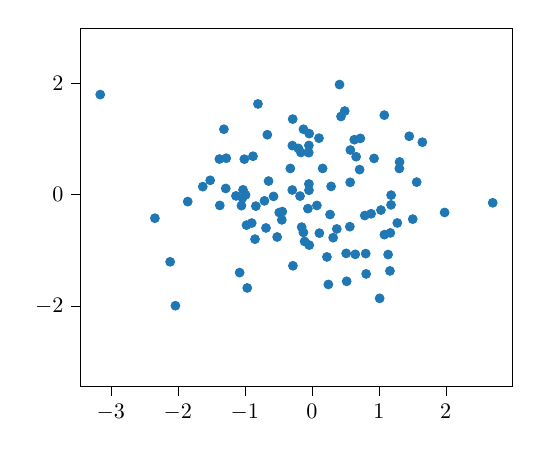
\begin{tikzpicture}[thick,scale=0.8, every node/.style={transform shape}]

\definecolor{color0}{rgb}{0.12156862745098,0.466666666666667,0.705882352941177}

\begin{axis}[
tick align=outside,
tick pos=left,
x grid style={white!69.0196078431373!black},
xmin=-3.45180709372072, xmax=2.99361349512875,
xtick style={color=black},
y grid style={white!69.0196078431373!black},
ymin=-3.45180709372072, ymax=2.99361349512875,
%ymin=-2.1938158082693, ymax=2.17815875977889,
ytick style={color=black}
]
\addplot [only marks, mark=*, draw=color0, fill=color0, colormap/viridis]
table{%
x                      y
-2.34275812782514 -0.422337072515164
0.24722747298104 -1.61319873633128
-1.38019830256552 0.640505435159906
-1.51714816067073 0.258502056354496
-0.175822267271081 -0.0252651026286875
-1.07790812289209 -1.40003857215438
1.08243752843236 1.42960529549044
1.45446356041819 1.05019519757262
0.272266762130476 -0.356289816160233
0.885609873179297 -0.34308175412289
0.318497415524185 -0.772246256656776
-0.486464599849546 -0.321047644667546
0.713664525872475 0.45089573918883
-3.15883343059119 1.79910626932364
1.03249205013434 -0.276218486658694
0.724867796410222 1.0119644513881
-0.66403264904207 1.07732210290748
-0.107877676726452 -0.840289685265736
1.01272382397982 -1.86298022827367
1.13929172816044 -1.07553705644164
-1.3126448374852 1.17645213621684
1.16650560208541 -1.36988664811057
-0.200901763190504 0.83207623547168
-0.162766483689669 0.758482159427621
-0.835280645501797 -0.205178137113613
-0.645878092492392 0.244918441252124
0.80474946774176 -1.05858981481516
0.520329697755992 -1.55654582504081
0.648482472610915 -1.07166832936951
0.512282026122496 -1.05460220157653
-1.62753042956307 0.144763499946151
-1.85256401192557 -0.124092650272665
-0.038308979791596 -0.906263941779864
2.70063983199922 -0.145679091954431
0.790570154320513 -0.374829753224335
-0.517513317388311 -0.760009533697624
0.567908869640562 -0.574932508687353
0.661942961282725 0.682717899396752
-0.897657764611887 -0.509805000910038
-0.125549177171554 -0.678365273082073
-0.878227336337594 0.691452914917409
-0.683949025620437 -0.59776859652354
-0.848312798273908 -0.798926002882831
0.112985819436421 -0.690906617864546
0.225572130815729 -1.11820672366738
1.30701775361222 0.471310001618085
1.17257671373237 -0.686628400040247
1.65057712884217 0.943486007801425
1.27651703162676 -0.507892465272379
1.18397678448062 -0.00794043507333255
0.491156506328976 1.50289694168447
-1.03569391216883 -0.0587326120757943
0.075771071420608 -0.192872784109992
-0.282308197205086 -1.27740706587447
-1.00748672473045 0.638365038742785
-1.27749128471686 0.65534756920239
-0.124824503595767 1.17650662278542
0.106611314555847 1.01602134591746
-1.13247270174148 -0.0219117447622604
-0.043848450781368 0.192488329289336
-0.0438948279215397 0.885200349964678
-0.0457880275415337 0.755095216844757
-1.28516929949252 0.112243759124342
-0.440817927077724 -0.304467240653771
0.161305007531463 0.47151626644206
-0.151580682549982 -0.582783939415887
-0.447730695225613 -0.452165071633186
0.372995023166489 -0.615248964656559
-0.707200164270895 -0.110920852624309
0.57264119973551 0.222410149332283
-0.291802622064795 0.0837691031769381
-2.03628199559491 -1.99508969153983
-2.11509949221634 -1.20644336802718
0.633895330915757 0.988721140629871
1.18243868402131 -0.182835421102174
1.56571290677136 0.226015644404297
1.50701998276123 -0.439351332338839
0.413852404170514 1.97943264304943
-0.285361579892089 1.35847512096702
-0.804429884793085 1.63103253934514
-0.058591464870352 -0.250495361764648
0.435590639323754 1.40570053244992
-0.320788003316259 0.471261823633868
0.287974042518776 0.149003002147366
0.811316786821193 -1.42384003157491
-0.96405415610173 -1.6757287701837
-1.02698880542662 0.0878139020675124
-1.05068784812419 -0.196660891853283
-1.37362659980222 -0.192873683671634
-0.0392455500475513 1.09768115355305
0.575537860345507 0.803161640917396
0.929214222549169 0.651745790327805
-0.97525635438475 -0.546892506013557
-0.042750903342611 0.0797462803574467
-0.290049580989981 0.882474726828786
1.08385271681253 -0.717881298334075
1.98268177645895 -0.319409301778917
1.31068071341738 0.588970190069706
-0.98887418389988 -0.00418003306320407
-0.571790491417394 -0.0307990540877851
};
\end{axis}

\end{tikzpicture}

\subcaption{Point cloud $S$.}
\end{center}
\end{subfigure}
\begin{subfigure}[t]{0.49\textwidth}
\begin{center}
% This file was created by tikzplotlib v0.9.2.
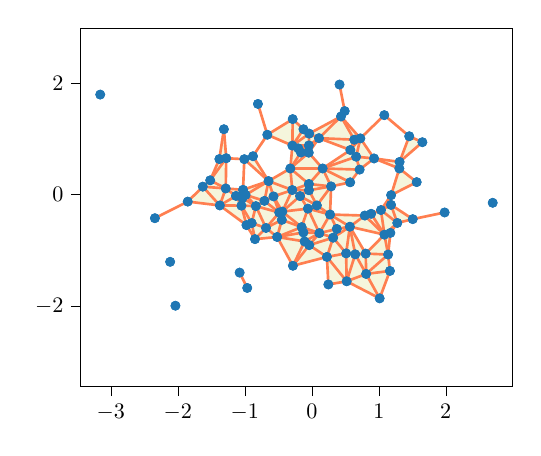
\begin{tikzpicture}[thick,scale=0.8, every node/.style={transform shape}]

\definecolor{color0}{rgb}{0.12156862745098,0.466666666666667,0.705882352941177}
\definecolor{color1}{rgb}{1,0.498039215686275,0.0549019607843137}
\definecolor{color2}{rgb}{0.96078431372549,0.96078431372549,0.862745098039216}
\definecolor{color3}{rgb}{1,0.498039215686275,0.313725490196078}

\begin{axis}[
tick align=outside,
tick pos=left,
x grid style={white!69.0196078431373!black},
xmin=-3.45180709372072, xmax=2.99361349512875,
xtick style={color=black},
y grid style={white!69.0196078431373!black},
ymin=-3.45180709372072, ymax=2.99361349512875,
%ymin=-2.1938158082693, ymax=2.17815875977889,
ytick style={color=black}
]
\addplot [only marks, mark=*, draw=color0, fill=color0, colormap/viridis]
table{%
x                      y
-2.34275812782514 -0.422337072515164
0.24722747298104 -1.61319873633128
-1.38019830256552 0.640505435159906
-1.51714816067073 0.258502056354496
-0.175822267271081 -0.0252651026286875
-1.07790812289209 -1.40003857215438
1.08243752843236 1.42960529549044
1.45446356041819 1.05019519757262
0.272266762130476 -0.356289816160233
0.885609873179297 -0.34308175412289
0.318497415524185 -0.772246256656776
-0.486464599849546 -0.321047644667546
0.713664525872475 0.45089573918883
-3.15883343059119 1.79910626932364
1.03249205013434 -0.276218486658694
0.724867796410222 1.0119644513881
-0.66403264904207 1.07732210290748
-0.107877676726452 -0.840289685265736
1.01272382397982 -1.86298022827367
1.13929172816044 -1.07553705644164
-1.3126448374852 1.17645213621684
1.16650560208541 -1.36988664811057
-0.200901763190504 0.83207623547168
-0.162766483689669 0.758482159427621
-0.835280645501797 -0.205178137113613
-0.645878092492392 0.244918441252124
0.80474946774176 -1.05858981481516
0.520329697755992 -1.55654582504081
0.648482472610915 -1.07166832936951
0.512282026122496 -1.05460220157653
-1.62753042956307 0.144763499946151
-1.85256401192557 -0.124092650272665
-0.038308979791596 -0.906263941779864
2.70063983199922 -0.145679091954431
0.790570154320513 -0.374829753224335
-0.517513317388311 -0.760009533697624
0.567908869640562 -0.574932508687353
0.661942961282725 0.682717899396752
-0.897657764611887 -0.509805000910038
-0.125549177171554 -0.678365273082073
-0.878227336337594 0.691452914917409
-0.683949025620437 -0.59776859652354
-0.848312798273908 -0.798926002882831
0.112985819436421 -0.690906617864546
0.225572130815729 -1.11820672366738
1.30701775361222 0.471310001618085
1.17257671373237 -0.686628400040247
1.65057712884217 0.943486007801425
1.27651703162676 -0.507892465272379
1.18397678448062 -0.00794043507333255
0.491156506328976 1.50289694168447
-1.03569391216883 -0.0587326120757943
0.075771071420608 -0.192872784109992
-0.282308197205086 -1.27740706587447
-1.00748672473045 0.638365038742785
-1.27749128471686 0.65534756920239
-0.124824503595767 1.17650662278542
0.106611314555847 1.01602134591746
-1.13247270174148 -0.0219117447622604
-0.043848450781368 0.192488329289336
-0.0438948279215397 0.885200349964678
-0.0457880275415337 0.755095216844757
-1.28516929949252 0.112243759124342
-0.440817927077724 -0.304467240653771
0.161305007531463 0.47151626644206
-0.151580682549982 -0.582783939415887
-0.447730695225613 -0.452165071633186
0.372995023166489 -0.615248964656559
-0.707200164270895 -0.110920852624309
0.57264119973551 0.222410149332283
-0.291802622064795 0.0837691031769381
-2.03628199559491 -1.99508969153983
-2.11509949221634 -1.20644336802718
0.633895330915757 0.988721140629871
1.18243868402131 -0.182835421102174
1.56571290677136 0.226015644404297
1.50701998276123 -0.439351332338839
0.413852404170514 1.97943264304943
-0.285361579892089 1.35847512096702
-0.804429884793085 1.63103253934514
-0.058591464870352 -0.250495361764648
0.435590639323754 1.40570053244992
-0.320788003316259 0.471261823633868
0.287974042518776 0.149003002147366
0.811316786821193 -1.42384003157491
-0.96405415610173 -1.6757287701837
-1.02698880542662 0.0878139020675124
-1.05068784812419 -0.196660891853283
-1.37362659980222 -0.192873683671634
-0.0392455500475513 1.09768115355305
0.575537860345507 0.803161640917396
0.929214222549169 0.651745790327805
-0.97525635438475 -0.546892506013557
-0.042750903342611 0.0797462803574467
-0.290049580989981 0.882474726828786
1.08385271681253 -0.717881298334075
1.98268177645895 -0.319409301778917
1.31068071341738 0.588970190069706
-0.98887418389988 -0.00418003306320407
-0.571790491417394 -0.0307990540877851
};
\path [draw=color2, fill=color2]
(axis cs:-0.486464599849546,-0.321047644667546)
--(axis cs:-0.440817927077724,-0.304467240653771)
--(axis cs:-0.447730695225613,-0.452165071633186)
--cycle;
\path [draw=color2, fill=color2]
(axis cs:-1.03569391216883,-0.0587326120757943)
--(axis cs:-1.13247270174148,-0.0219117447622604)
--(axis cs:-0.98887418389988,-0.00418003306320407)
--cycle;
\path [draw=color2, fill=color2]
(axis cs:-1.13247270174148,-0.0219117447622604)
--(axis cs:-1.02698880542662,0.0878139020675124)
--(axis cs:-0.98887418389988,-0.00418003306320407)
--cycle;
\path [draw=color2, fill=color2]
(axis cs:-0.162766483689669,0.758482159427621)
--(axis cs:-0.0438948279215397,0.885200349964678)
--(axis cs:-0.0457880275415337,0.755095216844757)
--cycle;
\path [draw=color2, fill=color2]
(axis cs:-0.200901763190504,0.83207623547168)
--(axis cs:-0.162766483689669,0.758482159427621)
--(axis cs:-0.0438948279215397,0.885200349964678)
--cycle;
\path [draw=color2, fill=color2]
(axis cs:-1.03569391216883,-0.0587326120757943)
--(axis cs:-1.13247270174148,-0.0219117447622604)
--(axis cs:-1.05068784812419,-0.196660891853283)
--cycle;
\path [draw=color2, fill=color2]
(axis cs:0.106611314555847,1.01602134591746)
--(axis cs:-0.0438948279215397,0.885200349964678)
--(axis cs:-0.0392455500475513,1.09768115355305)
--cycle;
\path [draw=color2, fill=color2]
(axis cs:-0.835280645501797,-0.205178137113613)
--(axis cs:-1.03569391216883,-0.0587326120757943)
--(axis cs:-1.05068784812419,-0.196660891853283)
--cycle;
\path [draw=color2, fill=color2]
(axis cs:-0.175822267271081,-0.0252651026286875)
--(axis cs:-0.291802622064795,0.0837691031769381)
--(axis cs:-0.042750903342611,0.0797462803574467)
--cycle;
\path [draw=color2, fill=color2]
(axis cs:-0.835280645501797,-0.205178137113613)
--(axis cs:-1.03569391216883,-0.0587326120757943)
--(axis cs:-0.98887418389988,-0.00418003306320407)
--cycle;
\path [draw=color2, fill=color2]
(axis cs:-1.13247270174148,-0.0219117447622604)
--(axis cs:-1.28516929949252,0.112243759124342)
--(axis cs:-1.02698880542662,0.0878139020675124)
--cycle;
\path [draw=color2, fill=color2]
(axis cs:-0.107877676726452,-0.840289685265736)
--(axis cs:-0.038308979791596,-0.906263941779864)
--(axis cs:0.112985819436421,-0.690906617864546)
--cycle;
\path [draw=color2, fill=color2]
(axis cs:-0.107877676726452,-0.840289685265736)
--(axis cs:-0.125549177171554,-0.678365273082073)
--(axis cs:0.112985819436421,-0.690906617864546)
--cycle;
\path [draw=color2, fill=color2]
(axis cs:-0.043848450781368,0.192488329289336)
--(axis cs:-0.291802622064795,0.0837691031769381)
--(axis cs:-0.042750903342611,0.0797462803574467)
--cycle;
\path [draw=color2, fill=color2]
(axis cs:0.318497415524185,-0.772246256656776)
--(axis cs:0.112985819436421,-0.690906617864546)
--(axis cs:0.372995023166489,-0.615248964656559)
--cycle;
\path [draw=color2, fill=color2]
(axis cs:-0.897657764611887,-0.509805000910038)
--(axis cs:-0.848312798273908,-0.798926002882831)
--(axis cs:-0.97525635438475,-0.546892506013557)
--cycle;
\path [draw=color2, fill=color2]
(axis cs:-0.125549177171554,-0.678365273082073)
--(axis cs:0.112985819436421,-0.690906617864546)
--(axis cs:-0.151580682549982,-0.582783939415887)
--cycle;
\path [draw=color2, fill=color2]
(axis cs:-0.835280645501797,-0.205178137113613)
--(axis cs:-0.707200164270895,-0.110920852624309)
--(axis cs:-0.98887418389988,-0.00418003306320407)
--cycle;
\path [draw=color2, fill=color2]
(axis cs:0.724867796410222,1.0119644513881)
--(axis cs:0.633895330915757,0.988721140629871)
--(axis cs:0.575537860345507,0.803161640917396)
--cycle;
\path [draw=color2, fill=color2]
(axis cs:-0.175822267271081,-0.0252651026286875)
--(axis cs:0.075771071420608,-0.192872784109992)
--(axis cs:-0.058591464870352,-0.250495361764648)
--cycle;
\path [draw=color2, fill=color2]
(axis cs:-0.486464599849546,-0.321047644667546)
--(axis cs:-0.440817927077724,-0.304467240653771)
--(axis cs:-0.571790491417394,-0.0307990540877851)
--cycle;
\path [draw=color2, fill=color2]
(axis cs:-0.897657764611887,-0.509805000910038)
--(axis cs:-0.683949025620437,-0.59776859652354)
--(axis cs:-0.848312798273908,-0.798926002882831)
--cycle;
\path [draw=color2, fill=color2]
(axis cs:0.713664525872475,0.45089573918883)
--(axis cs:0.661942961282725,0.682717899396752)
--(axis cs:0.929214222549169,0.651745790327805)
--cycle;
\path [draw=color2, fill=color2]
(axis cs:-0.175822267271081,-0.0252651026286875)
--(axis cs:0.075771071420608,-0.192872784109992)
--(axis cs:-0.042750903342611,0.0797462803574467)
--cycle;
\path [draw=color2, fill=color2]
(axis cs:-0.486464599849546,-0.321047644667546)
--(axis cs:-0.707200164270895,-0.110920852624309)
--(axis cs:-0.571790491417394,-0.0307990540877851)
--cycle;
\path [draw=color2, fill=color2]
(axis cs:-0.200901763190504,0.83207623547168)
--(axis cs:-0.162766483689669,0.758482159427621)
--(axis cs:-0.290049580989981,0.882474726828786)
--cycle;
\path [draw=color2, fill=color2]
(axis cs:-0.517513317388311,-0.760009533697624)
--(axis cs:-0.683949025620437,-0.59776859652354)
--(axis cs:-0.447730695225613,-0.452165071633186)
--cycle;
\path [draw=color2, fill=color2]
(axis cs:-1.13247270174148,-0.0219117447622604)
--(axis cs:-1.28516929949252,0.112243759124342)
--(axis cs:-1.37362659980222,-0.192873683671634)
--cycle;
\path [draw=color2, fill=color2]
(axis cs:-1.13247270174148,-0.0219117447622604)
--(axis cs:-1.05068784812419,-0.196660891853283)
--(axis cs:-1.37362659980222,-0.192873683671634)
--cycle;
\path [draw=color2, fill=color2]
(axis cs:-0.200901763190504,0.83207623547168)
--(axis cs:-0.0438948279215397,0.885200349964678)
--(axis cs:-0.290049580989981,0.882474726828786)
--cycle;
\path [draw=color2, fill=color2]
(axis cs:-0.0438948279215397,0.885200349964678)
--(axis cs:-0.0392455500475513,1.09768115355305)
--(axis cs:-0.290049580989981,0.882474726828786)
--cycle;
\path [draw=color2, fill=color2]
(axis cs:-0.517513317388311,-0.760009533697624)
--(axis cs:-0.683949025620437,-0.59776859652354)
--(axis cs:-0.848312798273908,-0.798926002882831)
--cycle;
\path [draw=color2, fill=color2]
(axis cs:-0.124824503595767,1.17650662278542)
--(axis cs:-0.0392455500475513,1.09768115355305)
--(axis cs:-0.290049580989981,0.882474726828786)
--cycle;
\path [draw=color2, fill=color2]
(axis cs:-0.043848450781368,0.192488329289336)
--(axis cs:0.287974042518776,0.149003002147366)
--(axis cs:-0.042750903342611,0.0797462803574467)
--cycle;
\path [draw=color2, fill=color2]
(axis cs:1.03249205013434,-0.276218486658694)
--(axis cs:1.27651703162676,-0.507892465272379)
--(axis cs:1.18243868402131,-0.182835421102174)
--cycle;
\path [draw=color2, fill=color2]
(axis cs:-1.51714816067073,0.258502056354496)
--(axis cs:-1.62753042956307,0.144763499946151)
--(axis cs:-1.28516929949252,0.112243759124342)
--cycle;
\path [draw=color2, fill=color2]
(axis cs:-0.486464599849546,-0.321047644667546)
--(axis cs:-0.683949025620437,-0.59776859652354)
--(axis cs:-0.447730695225613,-0.452165071633186)
--cycle;
\path [draw=color2, fill=color2]
(axis cs:-0.835280645501797,-0.205178137113613)
--(axis cs:-0.897657764611887,-0.509805000910038)
--(axis cs:-1.05068784812419,-0.196660891853283)
--cycle;
\path [draw=color2, fill=color2]
(axis cs:0.724867796410222,1.0119644513881)
--(axis cs:0.661942961282725,0.682717899396752)
--(axis cs:0.575537860345507,0.803161640917396)
--cycle;
\path [draw=color2, fill=color2]
(axis cs:-0.897657764611887,-0.509805000910038)
--(axis cs:-1.05068784812419,-0.196660891853283)
--(axis cs:-0.97525635438475,-0.546892506013557)
--cycle;
\path [draw=color2, fill=color2]
(axis cs:1.03249205013434,-0.276218486658694)
--(axis cs:1.18397678448062,-0.00794043507333255)
--(axis cs:1.18243868402131,-0.182835421102174)
--cycle;
\path [draw=color2, fill=color2]
(axis cs:0.318497415524185,-0.772246256656776)
--(axis cs:0.567908869640562,-0.574932508687353)
--(axis cs:0.372995023166489,-0.615248964656559)
--cycle;
\path [draw=color2, fill=color2]
(axis cs:0.272266762130476,-0.356289816160233)
--(axis cs:0.112985819436421,-0.690906617864546)
--(axis cs:0.372995023166489,-0.615248964656559)
--cycle;
\path [draw=color2, fill=color2]
(axis cs:0.272266762130476,-0.356289816160233)
--(axis cs:0.567908869640562,-0.574932508687353)
--(axis cs:0.372995023166489,-0.615248964656559)
--cycle;
\path [draw=color2, fill=color2]
(axis cs:-0.486464599849546,-0.321047644667546)
--(axis cs:-0.835280645501797,-0.205178137113613)
--(axis cs:-0.707200164270895,-0.110920852624309)
--cycle;
\path [draw=color2, fill=color2]
(axis cs:-0.645878092492392,0.244918441252124)
--(axis cs:-0.707200164270895,-0.110920852624309)
--(axis cs:-0.571790491417394,-0.0307990540877851)
--cycle;
\path [draw=color2, fill=color2]
(axis cs:0.318497415524185,-0.772246256656776)
--(axis cs:0.512282026122496,-1.05460220157653)
--(axis cs:0.225572130815729,-1.11820672366738)
--cycle;
\path [draw=color2, fill=color2]
(axis cs:0.80474946774176,-1.05858981481516)
--(axis cs:0.648482472610915,-1.07166832936951)
--(axis cs:0.811316786821193,-1.42384003157491)
--cycle;
\path [draw=color2, fill=color2]
(axis cs:0.272266762130476,-0.356289816160233)
--(axis cs:0.075771071420608,-0.192872784109992)
--(axis cs:-0.058591464870352,-0.250495361764648)
--cycle;
\path [draw=color2, fill=color2]
(axis cs:0.318497415524185,-0.772246256656776)
--(axis cs:-0.038308979791596,-0.906263941779864)
--(axis cs:0.112985819436421,-0.690906617864546)
--cycle;
\path [draw=color2, fill=color2]
(axis cs:-0.645878092492392,0.244918441252124)
--(axis cs:-0.291802622064795,0.0837691031769381)
--(axis cs:-0.571790491417394,-0.0307990540877851)
--cycle;
\path [draw=color2, fill=color2]
(axis cs:-0.043848450781368,0.192488329289336)
--(axis cs:0.161305007531463,0.47151626644206)
--(axis cs:0.287974042518776,0.149003002147366)
--cycle;
\path [draw=color2, fill=color2]
(axis cs:1.13929172816044,-1.07553705644164)
--(axis cs:1.17257671373237,-0.686628400040247)
--(axis cs:1.08385271681253,-0.717881298334075)
--cycle;
\path [draw=color2, fill=color2]
(axis cs:0.106611314555847,1.01602134591746)
--(axis cs:-0.0438948279215397,0.885200349964678)
--(axis cs:-0.0457880275415337,0.755095216844757)
--cycle;
\path [draw=color2, fill=color2]
(axis cs:-0.517513317388311,-0.760009533697624)
--(axis cs:-0.125549177171554,-0.678365273082073)
--(axis cs:-0.151580682549982,-0.582783939415887)
--cycle;
\path [draw=color2, fill=color2]
(axis cs:-0.175822267271081,-0.0252651026286875)
--(axis cs:-0.440817927077724,-0.304467240653771)
--(axis cs:-0.058591464870352,-0.250495361764648)
--cycle;
\path [draw=color2, fill=color2]
(axis cs:0.075771071420608,-0.192872784109992)
--(axis cs:0.287974042518776,0.149003002147366)
--(axis cs:-0.042750903342611,0.0797462803574467)
--cycle;
\path [draw=color2, fill=color2]
(axis cs:1.27651703162676,-0.507892465272379)
--(axis cs:1.18243868402131,-0.182835421102174)
--(axis cs:1.50701998276123,-0.439351332338839)
--cycle;
\path [draw=color2, fill=color2]
(axis cs:-0.517513317388311,-0.760009533697624)
--(axis cs:-0.151580682549982,-0.582783939415887)
--(axis cs:-0.447730695225613,-0.452165071633186)
--cycle;
\path [draw=color2, fill=color2]
(axis cs:0.724867796410222,1.0119644513881)
--(axis cs:0.661942961282725,0.682717899396752)
--(axis cs:0.929214222549169,0.651745790327805)
--cycle;
\path [draw=color2, fill=color2]
(axis cs:-0.175822267271081,-0.0252651026286875)
--(axis cs:-0.440817927077724,-0.304467240653771)
--(axis cs:-0.291802622064795,0.0837691031769381)
--cycle;
\path [draw=color2, fill=color2]
(axis cs:0.318497415524185,-0.772246256656776)
--(axis cs:-0.038308979791596,-0.906263941779864)
--(axis cs:0.225572130815729,-1.11820672366738)
--cycle;
\path [draw=color2, fill=color2]
(axis cs:-0.440817927077724,-0.304467240653771)
--(axis cs:-0.291802622064795,0.0837691031769381)
--(axis cs:-0.571790491417394,-0.0307990540877851)
--cycle;
\path [draw=color2, fill=color2]
(axis cs:-0.043848450781368,0.192488329289336)
--(axis cs:-0.291802622064795,0.0837691031769381)
--(axis cs:-0.320788003316259,0.471261823633868)
--cycle;
\path [draw=color2, fill=color2]
(axis cs:-0.107877676726452,-0.840289685265736)
--(axis cs:-0.517513317388311,-0.760009533697624)
--(axis cs:-0.125549177171554,-0.678365273082073)
--cycle;
\path [draw=color2, fill=color2]
(axis cs:1.30701775361222,0.471310001618085)
--(axis cs:0.929214222549169,0.651745790327805)
--(axis cs:1.31068071341738,0.588970190069706)
--cycle;
\path [draw=color2, fill=color2]
(axis cs:-0.645878092492392,0.244918441252124)
--(axis cs:-1.02698880542662,0.0878139020675124)
--(axis cs:-0.98887418389988,-0.00418003306320407)
--cycle;
\path [draw=color2, fill=color2]
(axis cs:-0.162766483689669,0.758482159427621)
--(axis cs:-0.320788003316259,0.471261823633868)
--(axis cs:-0.290049580989981,0.882474726828786)
--cycle;
\path [draw=color2, fill=color2]
(axis cs:-0.835280645501797,-0.205178137113613)
--(axis cs:-0.897657764611887,-0.509805000910038)
--(axis cs:-0.683949025620437,-0.59776859652354)
--cycle;
\path [draw=color2, fill=color2]
(axis cs:-1.62753042956307,0.144763499946151)
--(axis cs:-1.28516929949252,0.112243759124342)
--(axis cs:-1.37362659980222,-0.192873683671634)
--cycle;
\path [draw=color2, fill=color2]
(axis cs:-0.440817927077724,-0.304467240653771)
--(axis cs:-0.151580682549982,-0.582783939415887)
--(axis cs:-0.447730695225613,-0.452165071633186)
--cycle;
\path [draw=color2, fill=color2]
(axis cs:-0.645878092492392,0.244918441252124)
--(axis cs:-0.707200164270895,-0.110920852624309)
--(axis cs:-0.98887418389988,-0.00418003306320407)
--cycle;
\path [draw=color2, fill=color2]
(axis cs:-0.440817927077724,-0.304467240653771)
--(axis cs:-0.151580682549982,-0.582783939415887)
--(axis cs:-0.058591464870352,-0.250495361764648)
--cycle;
\path [draw=color2, fill=color2]
(axis cs:1.17257671373237,-0.686628400040247)
--(axis cs:1.27651703162676,-0.507892465272379)
--(axis cs:1.08385271681253,-0.717881298334075)
--cycle;
\path [draw=color2, fill=color2]
(axis cs:-0.486464599849546,-0.321047644667546)
--(axis cs:-0.835280645501797,-0.205178137113613)
--(axis cs:-0.683949025620437,-0.59776859652354)
--cycle;
\path [draw=color2, fill=color2]
(axis cs:-0.162766483689669,0.758482159427621)
--(axis cs:-0.0457880275415337,0.755095216844757)
--(axis cs:-0.320788003316259,0.471261823633868)
--cycle;
\path [draw=color2, fill=color2]
(axis cs:1.03249205013434,-0.276218486658694)
--(axis cs:1.27651703162676,-0.507892465272379)
--(axis cs:1.08385271681253,-0.717881298334075)
--cycle;
\path [draw=color2, fill=color2]
(axis cs:0.885609873179297,-0.34308175412289)
--(axis cs:1.03249205013434,-0.276218486658694)
--(axis cs:1.08385271681253,-0.717881298334075)
--cycle;
\path [draw=color2, fill=color2]
(axis cs:1.13929172816044,-1.07553705644164)
--(axis cs:0.80474946774176,-1.05858981481516)
--(axis cs:1.08385271681253,-0.717881298334075)
--cycle;
\path [draw=color2, fill=color2]
(axis cs:-0.645878092492392,0.244918441252124)
--(axis cs:-0.291802622064795,0.0837691031769381)
--(axis cs:-0.320788003316259,0.471261823633868)
--cycle;
\path [draw=color2, fill=color2]
(axis cs:0.885609873179297,-0.34308175412289)
--(axis cs:0.790570154320513,-0.374829753224335)
--(axis cs:1.08385271681253,-0.717881298334075)
--cycle;
\path [draw=color2, fill=color2]
(axis cs:0.112985819436421,-0.690906617864546)
--(axis cs:-0.151580682549982,-0.582783939415887)
--(axis cs:-0.058591464870352,-0.250495361764648)
--cycle;
\path [draw=color2, fill=color2]
(axis cs:0.272266762130476,-0.356289816160233)
--(axis cs:0.112985819436421,-0.690906617864546)
--(axis cs:-0.058591464870352,-0.250495361764648)
--cycle;
\path [draw=color2, fill=color2]
(axis cs:-0.107877676726452,-0.840289685265736)
--(axis cs:-0.038308979791596,-0.906263941779864)
--(axis cs:-0.282308197205086,-1.27740706587447)
--cycle;
\path [draw=color2, fill=color2]
(axis cs:1.13929172816044,-1.07553705644164)
--(axis cs:1.16650560208541,-1.36988664811057)
--(axis cs:0.811316786821193,-1.42384003157491)
--cycle;
\path [draw=color2, fill=color2]
(axis cs:1.13929172816044,-1.07553705644164)
--(axis cs:0.80474946774176,-1.05858981481516)
--(axis cs:0.811316786821193,-1.42384003157491)
--cycle;
\path [draw=color2, fill=color2]
(axis cs:0.318497415524185,-0.772246256656776)
--(axis cs:0.512282026122496,-1.05460220157653)
--(axis cs:0.567908869640562,-0.574932508687353)
--cycle;
\path [draw=color2, fill=color2]
(axis cs:0.161305007531463,0.47151626644206)
--(axis cs:0.57264119973551,0.222410149332283)
--(axis cs:0.287974042518776,0.149003002147366)
--cycle;
\path [draw=color2, fill=color2]
(axis cs:-0.043848450781368,0.192488329289336)
--(axis cs:0.161305007531463,0.47151626644206)
--(axis cs:-0.320788003316259,0.471261823633868)
--cycle;
\path [draw=color2, fill=color2]
(axis cs:-0.0457880275415337,0.755095216844757)
--(axis cs:0.161305007531463,0.47151626644206)
--(axis cs:-0.320788003316259,0.471261823633868)
--cycle;
\path [draw=color2, fill=color2]
(axis cs:-1.62753042956307,0.144763499946151)
--(axis cs:-1.85256401192557,-0.124092650272665)
--(axis cs:-1.37362659980222,-0.192873683671634)
--cycle;
\path [draw=color2, fill=color2]
(axis cs:0.724867796410222,1.0119644513881)
--(axis cs:0.633895330915757,0.988721140629871)
--(axis cs:0.435590639323754,1.40570053244992)
--cycle;
\path [draw=color2, fill=color2]
(axis cs:1.45446356041819,1.05019519757262)
--(axis cs:1.65057712884217,0.943486007801425)
--(axis cs:1.31068071341738,0.588970190069706)
--cycle;
\path [draw=color2, fill=color2]
(axis cs:0.520329697755992,-1.55654582504081)
--(axis cs:0.648482472610915,-1.07166832936951)
--(axis cs:0.811316786821193,-1.42384003157491)
--cycle;
\path [draw=color2, fill=color2]
(axis cs:0.648482472610915,-1.07166832936951)
--(axis cs:0.512282026122496,-1.05460220157653)
--(axis cs:0.567908869640562,-0.574932508687353)
--cycle;
\path [draw=color2, fill=color2]
(axis cs:-0.124824503595767,1.17650662278542)
--(axis cs:-0.285361579892089,1.35847512096702)
--(axis cs:-0.290049580989981,0.882474726828786)
--cycle;
\path [draw=color2, fill=color2]
(axis cs:0.520329697755992,-1.55654582504081)
--(axis cs:0.648482472610915,-1.07166832936951)
--(axis cs:0.512282026122496,-1.05460220157653)
--cycle;
\path [draw=color2, fill=color2]
(axis cs:0.272266762130476,-0.356289816160233)
--(axis cs:0.075771071420608,-0.192872784109992)
--(axis cs:0.287974042518776,0.149003002147366)
--cycle;
\path [draw=color2, fill=color2]
(axis cs:1.30701775361222,0.471310001618085)
--(axis cs:1.18397678448062,-0.00794043507333255)
--(axis cs:1.56571290677136,0.226015644404297)
--cycle;
\path [draw=color2, fill=color2]
(axis cs:-1.38019830256552,0.640505435159906)
--(axis cs:-1.51714816067073,0.258502056354496)
--(axis cs:-1.27749128471686,0.65534756920239)
--cycle;
\path [draw=color2, fill=color2]
(axis cs:-0.66403264904207,1.07732210290748)
--(axis cs:-0.285361579892089,1.35847512096702)
--(axis cs:-0.290049580989981,0.882474726828786)
--cycle;
\path [draw=color2, fill=color2]
(axis cs:0.272266762130476,-0.356289816160233)
--(axis cs:0.790570154320513,-0.374829753224335)
--(axis cs:0.567908869640562,-0.574932508687353)
--cycle;
\path [draw=color2, fill=color2]
(axis cs:0.106611314555847,1.01602134591746)
--(axis cs:0.633895330915757,0.988721140629871)
--(axis cs:0.575537860345507,0.803161640917396)
--cycle;
\path [draw=color2, fill=color2]
(axis cs:-0.038308979791596,-0.906263941779864)
--(axis cs:0.225572130815729,-1.11820672366738)
--(axis cs:-0.282308197205086,-1.27740706587447)
--cycle;
\path [draw=color2, fill=color2]
(axis cs:0.24722747298104,-1.61319873633128)
--(axis cs:0.520329697755992,-1.55654582504081)
--(axis cs:0.225572130815729,-1.11820672366738)
--cycle;
\path [draw=color2, fill=color2]
(axis cs:0.790570154320513,-0.374829753224335)
--(axis cs:0.567908869640562,-0.574932508687353)
--(axis cs:1.08385271681253,-0.717881298334075)
--cycle;
\path [draw=color2, fill=color2]
(axis cs:-0.645878092492392,0.244918441252124)
--(axis cs:-0.878227336337594,0.691452914917409)
--(axis cs:-1.00748672473045,0.638365038742785)
--cycle;
\path [draw=color2, fill=color2]
(axis cs:1.01272382397982,-1.86298022827367)
--(axis cs:1.16650560208541,-1.36988664811057)
--(axis cs:0.811316786821193,-1.42384003157491)
--cycle;
\path [draw=color2, fill=color2]
(axis cs:0.520329697755992,-1.55654582504081)
--(axis cs:0.512282026122496,-1.05460220157653)
--(axis cs:0.225572130815729,-1.11820672366738)
--cycle;
\path [draw=color2, fill=color2]
(axis cs:0.80474946774176,-1.05858981481516)
--(axis cs:0.648482472610915,-1.07166832936951)
--(axis cs:0.567908869640562,-0.574932508687353)
--cycle;
\path [draw=color2, fill=color2]
(axis cs:-1.38019830256552,0.640505435159906)
--(axis cs:-1.3126448374852,1.17645213621684)
--(axis cs:-1.27749128471686,0.65534756920239)
--cycle;
\path [draw=color2, fill=color2]
(axis cs:-1.51714816067073,0.258502056354496)
--(axis cs:-1.27749128471686,0.65534756920239)
--(axis cs:-1.28516929949252,0.112243759124342)
--cycle;
\path [draw=color2, fill=color2]
(axis cs:0.661942961282725,0.682717899396752)
--(axis cs:0.161305007531463,0.47151626644206)
--(axis cs:0.575537860345507,0.803161640917396)
--cycle;
\path [draw=color2, fill=color2]
(axis cs:-1.05068784812419,-0.196660891853283)
--(axis cs:-1.37362659980222,-0.192873683671634)
--(axis cs:-0.97525635438475,-0.546892506013557)
--cycle;
\path [draw=color2, fill=color2]
(axis cs:0.713664525872475,0.45089573918883)
--(axis cs:0.161305007531463,0.47151626644206)
--(axis cs:0.57264119973551,0.222410149332283)
--cycle;
\path [draw=color2, fill=color2]
(axis cs:0.713664525872475,0.45089573918883)
--(axis cs:0.661942961282725,0.682717899396752)
--(axis cs:0.161305007531463,0.47151626644206)
--cycle;
\path [draw=color2, fill=color2]
(axis cs:0.106611314555847,1.01602134591746)
--(axis cs:0.435590639323754,1.40570053244992)
--(axis cs:-0.0392455500475513,1.09768115355305)
--cycle;
\path [draw=color2, fill=color2]
(axis cs:-0.107877676726452,-0.840289685265736)
--(axis cs:-0.517513317388311,-0.760009533697624)
--(axis cs:-0.282308197205086,-1.27740706587447)
--cycle;
\path [draw=color2, fill=color2]
(axis cs:0.106611314555847,1.01602134591746)
--(axis cs:0.633895330915757,0.988721140629871)
--(axis cs:0.435590639323754,1.40570053244992)
--cycle;
\path [draw=color2, fill=color2]
(axis cs:1.01272382397982,-1.86298022827367)
--(axis cs:0.520329697755992,-1.55654582504081)
--(axis cs:0.811316786821193,-1.42384003157491)
--cycle;
\addplot [very thick, color3]
table {%
-0.486464599849546 -0.321047644667546
-0.440817927077724 -0.304467240653771
};
\addplot [very thick, color3]
table {%
-1.03569391216883 -0.0587326120757943
-0.98887418389988 -0.00418003306320407
};
\addplot [very thick, color3]
table {%
-0.200901763190504 0.83207623547168
-0.162766483689669 0.758482159427621
};
\addplot [very thick, color3]
table {%
-0.897657764611887 -0.509805000910038
-0.97525635438475 -0.546892506013557
};
\addplot [very thick, color3]
table {%
0.724867796410222 1.0119644513881
0.633895330915757 0.988721140629871
};
\addplot [very thick, color3]
table {%
1.17257671373237 -0.686628400040247
1.08385271681253 -0.717881298334075
};
\addplot [very thick, color3]
table {%
-0.107877676726452 -0.840289685265736
-0.038308979791596 -0.906263941779864
};
\addplot [very thick, color3]
table {%
-0.125549177171554 -0.678365273082073
-0.151580682549982 -0.582783939415887
};
\addplot [very thick, color3]
table {%
-1.02698880542662 0.0878139020675124
-0.98887418389988 -0.00418003306320407
};
\addplot [very thick, color3]
table {%
0.885609873179297 -0.34308175412289
0.790570154320513 -0.374829753224335
};
\addplot [very thick, color3]
table {%
-0.200901763190504 0.83207623547168
-0.290049580989981 0.882474726828786
};
\addplot [very thick, color3]
table {%
-1.03569391216883 -0.0587326120757943
-1.13247270174148 -0.0219117447622604
};
\addplot [very thick, color3]
table {%
-1.38019830256552 0.640505435159906
-1.27749128471686 0.65534756920239
};
\addplot [very thick, color3]
table {%
0.491156506328976 1.50289694168447
0.435590639323754 1.40570053244992
};
\addplot [very thick, color3]
table {%
-0.043848450781368 0.192488329289336
-0.042750903342611 0.0797462803574467
};
\addplot [very thick, color3]
table {%
-0.124824503595767 1.17650662278542
-0.0392455500475513 1.09768115355305
};
\addplot [very thick, color3]
table {%
-0.162766483689669 0.758482159427621
-0.0457880275415337 0.755095216844757
};
\addplot [very thick, color3]
table {%
1.30701775361222 0.471310001618085
1.31068071341738 0.588970190069706
};
\addplot [very thick, color3]
table {%
-0.0438948279215397 0.885200349964678
-0.0457880275415337 0.755095216844757
};
\addplot [very thick, color3]
table {%
-0.486464599849546 -0.321047644667546
-0.447730695225613 -0.452165071633186
};
\addplot [very thick, color3]
table {%
0.648482472610915 -1.07166832936951
0.512282026122496 -1.05460220157653
};
\addplot [very thick, color3]
table {%
-1.03569391216883 -0.0587326120757943
-1.05068784812419 -0.196660891853283
};
\addplot [very thick, color3]
table {%
-0.878227336337594 0.691452914917409
-1.00748672473045 0.638365038742785
};
\addplot [very thick, color3]
table {%
0.075771071420608 -0.192872784109992
-0.058591464870352 -0.250495361764648
};
\addplot [very thick, color3]
table {%
-0.440817927077724 -0.304467240653771
-0.447730695225613 -0.452165071633186
};
\addplot [very thick, color3]
table {%
0.661942961282725 0.682717899396752
0.575537860345507 0.803161640917396
};
\addplot [very thick, color3]
table {%
-1.13247270174148 -0.0219117447622604
-1.02698880542662 0.0878139020675124
};
\addplot [very thick, color3]
table {%
-1.13247270174148 -0.0219117447622604
-0.98887418389988 -0.00418003306320407
};
\addplot [very thick, color3]
table {%
0.80474946774176 -1.05858981481516
0.648482472610915 -1.07166832936951
};
\addplot [very thick, color3]
table {%
-0.707200164270895 -0.110920852624309
-0.571790491417394 -0.0307990540877851
};
\addplot [very thick, color3]
table {%
-1.51714816067073 0.258502056354496
-1.62753042956307 0.144763499946151
};
\addplot [very thick, color3]
table {%
-0.835280645501797 -0.205178137113613
-0.707200164270895 -0.110920852624309
};
\addplot [very thick, color3]
table {%
-0.175822267271081 -0.0252651026286875
-0.291802622064795 0.0837691031769381
};
\addplot [very thick, color3]
table {%
0.885609873179297 -0.34308175412289
1.03249205013434 -0.276218486658694
};
\addplot [very thick, color3]
table {%
-0.107877676726452 -0.840289685265736
-0.125549177171554 -0.678365273082073
};
\addplot [very thick, color3]
table {%
-0.200901763190504 0.83207623547168
-0.0438948279215397 0.885200349964678
};
\addplot [very thick, color3]
table {%
0.318497415524185 -0.772246256656776
0.372995023166489 -0.615248964656559
};
\addplot [very thick, color3]
table {%
0.106611314555847 1.01602134591746
-0.0392455500475513 1.09768115355305
};
\addplot [very thick, color3]
table {%
-0.175822267271081 -0.0252651026286875
-0.042750903342611 0.0797462803574467
};
\addplot [very thick, color3]
table {%
-0.162766483689669 0.758482159427621
-0.0438948279215397 0.885200349964678
};
\addplot [very thick, color3]
table {%
1.18397678448062 -0.00794043507333255
1.18243868402131 -0.182835421102174
};
\addplot [very thick, color3]
table {%
1.03249205013434 -0.276218486658694
1.18243868402131 -0.182835421102174
};
\addplot [very thick, color3]
table {%
0.633895330915757 0.988721140629871
0.575537860345507 0.803161640917396
};
\addplot [very thick, color3]
table {%
0.567908869640562 -0.574932508687353
0.372995023166489 -0.615248964656559
};
\addplot [very thick, color3]
table {%
-1.13247270174148 -0.0219117447622604
-1.05068784812419 -0.196660891853283
};
\addplot [very thick, color3]
table {%
0.106611314555847 1.01602134591746
-0.0438948279215397 0.885200349964678
};
\addplot [very thick, color3]
table {%
-1.13247270174148 -0.0219117447622604
-1.28516929949252 0.112243759124342
};
\addplot [very thick, color3]
table {%
1.17257671373237 -0.686628400040247
1.27651703162676 -0.507892465272379
};
\addplot [very thick, color3]
table {%
-0.0438948279215397 0.885200349964678
-0.0392455500475513 1.09768115355305
};
\addplot [very thick, color3]
table {%
-0.835280645501797 -0.205178137113613
-1.05068784812419 -0.196660891853283
};
\addplot [very thick, color3]
table {%
0.318497415524185 -0.772246256656776
0.112985819436421 -0.690906617864546
};
\addplot [very thick, color3]
table {%
1.45446356041819 1.05019519757262
1.65057712884217 0.943486007801425
};
\addplot [very thick, color3]
table {%
-0.897657764611887 -0.509805000910038
-0.683949025620437 -0.59776859652354
};
\addplot [very thick, color3]
table {%
-0.517513317388311 -0.760009533697624
-0.683949025620437 -0.59776859652354
};
\addplot [very thick, color3]
table {%
0.713664525872475 0.45089573918883
0.661942961282725 0.682717899396752
};
\addplot [very thick, color3]
table {%
-0.125549177171554 -0.678365273082073
0.112985819436421 -0.690906617864546
};
\addplot [very thick, color3]
table {%
1.27651703162676 -0.507892465272379
1.50701998276123 -0.439351332338839
};
\addplot [very thick, color3]
table {%
-0.124824503595767 1.17650662278542
-0.285361579892089 1.35847512096702
};
\addplot [very thick, color3]
table {%
-0.835280645501797 -0.205178137113613
-1.03569391216883 -0.0587326120757943
};
\addplot [very thick, color3]
table {%
-0.291802622064795 0.0837691031769381
-0.042750903342611 0.0797462803574467
};
\addplot [very thick, color3]
table {%
-0.835280645501797 -0.205178137113613
-0.98887418389988 -0.00418003306320407
};
\addplot [very thick, color3]
table {%
-0.175822267271081 -0.0252651026286875
-0.058591464870352 -0.250495361764648
};
\addplot [very thick, color3]
table {%
0.272266762130476 -0.356289816160233
0.075771071420608 -0.192872784109992
};
\addplot [very thick, color3]
table {%
-1.28516929949252 0.112243759124342
-1.02698880542662 0.0878139020675124
};
\addplot [very thick, color3]
table {%
-0.683949025620437 -0.59776859652354
-0.848312798273908 -0.798926002882831
};
\addplot [very thick, color3]
table {%
-0.038308979791596 -0.906263941779864
0.112985819436421 -0.690906617864546
};
\addplot [very thick, color3]
table {%
-0.107877676726452 -0.840289685265736
0.112985819436421 -0.690906617864546
};
\addplot [very thick, color3]
table {%
0.713664525872475 0.45089573918883
0.57264119973551 0.222410149332283
};
\addplot [very thick, color3]
table {%
0.661942961282725 0.682717899396752
0.929214222549169 0.651745790327805
};
\addplot [very thick, color3]
table {%
-1.00748672473045 0.638365038742785
-1.27749128471686 0.65534756920239
};
\addplot [very thick, color3]
table {%
-0.043848450781368 0.192488329289336
-0.291802622064795 0.0837691031769381
};
\addplot [very thick, color3]
table {%
0.112985819436421 -0.690906617864546
0.372995023166489 -0.615248964656559
};
\addplot [very thick, color3]
table {%
-1.51714816067073 0.258502056354496
-1.28516929949252 0.112243759124342
};
\addplot [very thick, color3]
table {%
-0.683949025620437 -0.59776859652354
-0.447730695225613 -0.452165071633186
};
\addplot [very thick, color3]
table {%
0.272266762130476 -0.356289816160233
0.372995023166489 -0.615248964656559
};
\addplot [very thick, color3]
table {%
0.24722747298104 -1.61319873633128
0.520329697755992 -1.55654582504081
};
\addplot [very thick, color3]
table {%
-0.848312798273908 -0.798926002882831
-0.97525635438475 -0.546892506013557
};
\addplot [very thick, color3]
table {%
-0.645878092492392 0.244918441252124
-0.571790491417394 -0.0307990540877851
};
\addplot [very thick, color3]
table {%
-0.897657764611887 -0.509805000910038
-0.848312798273908 -0.798926002882831
};
\addplot [very thick, color3]
table {%
0.512282026122496 -1.05460220157653
0.225572130815729 -1.11820672366738
};
\addplot [very thick, color3]
table {%
0.57264119973551 0.222410149332283
0.287974042518776 0.149003002147366
};
\addplot [very thick, color3]
table {%
0.713664525872475 0.45089573918883
0.929214222549169 0.651745790327805
};
\addplot [very thick, color3]
table {%
1.13929172816044 -1.07553705644164
1.16650560208541 -1.36988664811057
};
\addplot [very thick, color3]
table {%
-1.13247270174148 -0.0219117447622604
-1.37362659980222 -0.192873683671634
};
\addplot [very thick, color3]
table {%
0.075771071420608 -0.192872784109992
-0.042750903342611 0.0797462803574467
};
\addplot [very thick, color3]
table {%
-1.07790812289209 -1.40003857215438
-0.96405415610173 -1.6757287701837
};
\addplot [very thick, color3]
table {%
0.790570154320513 -0.374829753224335
0.567908869640562 -0.574932508687353
};
\addplot [very thick, color3]
table {%
0.112985819436421 -0.690906617864546
-0.151580682549982 -0.582783939415887
};
\addplot [very thick, color3]
table {%
-0.707200164270895 -0.110920852624309
-0.98887418389988 -0.00418003306320407
};
\addplot [very thick, color3]
table {%
0.724867796410222 1.0119644513881
0.575537860345507 0.803161640917396
};
\addplot [very thick, color3]
table {%
-0.291802622064795 0.0837691031769381
-0.571790491417394 -0.0307990540877851
};
\addplot [very thick, color3]
table {%
-0.486464599849546 -0.321047644667546
-0.571790491417394 -0.0307990540877851
};
\addplot [very thick, color3]
table {%
-0.175822267271081 -0.0252651026286875
0.075771071420608 -0.192872784109992
};
\addplot [very thick, color3]
table {%
-0.440817927077724 -0.304467240653771
-0.571790491417394 -0.0307990540877851
};
\addplot [very thick, color3]
table {%
-0.486464599849546 -0.321047644667546
-0.707200164270895 -0.110920852624309
};
\addplot [very thick, color3]
table {%
-0.835280645501797 -0.205178137113613
-0.897657764611887 -0.509805000910038
};
\addplot [very thick, color3]
table {%
-0.517513317388311 -0.760009533697624
-0.447730695225613 -0.452165071633186
};
\addplot [very thick, color3]
table {%
-1.28516929949252 0.112243759124342
-1.37362659980222 -0.192873683671634
};
\addplot [very thick, color3]
table {%
0.520329697755992 -1.55654582504081
0.811316786821193 -1.42384003157491
};
\addplot [very thick, color3]
table {%
-1.05068784812419 -0.196660891853283
-1.37362659980222 -0.192873683671634
};
\addplot [very thick, color3]
table {%
-0.151580682549982 -0.582783939415887
-0.447730695225613 -0.452165071633186
};
\addplot [very thick, color3]
table {%
-0.162766483689669 0.758482159427621
-0.290049580989981 0.882474726828786
};
\addplot [very thick, color3]
table {%
-0.162766483689669 0.758482159427621
-0.320788003316259 0.471261823633868
};
\addplot [very thick, color3]
table {%
-0.0438948279215397 0.885200349964678
-0.290049580989981 0.882474726828786
};
\addplot [very thick, color3]
table {%
-0.0392455500475513 1.09768115355305
-0.290049580989981 0.882474726828786
};
\addplot [very thick, color3]
table {%
-0.517513317388311 -0.760009533697624
-0.848312798273908 -0.798926002882831
};
\addplot [very thick, color3]
table {%
-0.043848450781368 0.192488329289336
0.287974042518776 0.149003002147366
};
\addplot [very thick, color3]
table {%
1.13929172816044 -1.07553705644164
0.80474946774176 -1.05858981481516
};
\addplot [very thick, color3]
table {%
1.03249205013434 -0.276218486658694
1.27651703162676 -0.507892465272379
};
\addplot [very thick, color3]
table {%
-0.124824503595767 1.17650662278542
-0.290049580989981 0.882474726828786
};
\addplot [very thick, color3]
table {%
0.287974042518776 0.149003002147366
-0.042750903342611 0.0797462803574467
};
\addplot [very thick, color3]
table {%
1.27651703162676 -0.507892465272379
1.18243868402131 -0.182835421102174
};
\addplot [very thick, color3]
table {%
-0.038308979791596 -0.906263941779864
0.225572130815729 -1.11820672366738
};
\addplot [very thick, color3]
table {%
0.318497415524185 -0.772246256656776
0.512282026122496 -1.05460220157653
};
\addplot [very thick, color3]
table {%
-0.151580682549982 -0.582783939415887
-0.058591464870352 -0.250495361764648
};
\addplot [very thick, color3]
table {%
-0.043848450781368 0.192488329289336
0.161305007531463 0.47151626644206
};
\addplot [very thick, color3]
table {%
0.161305007531463 0.47151626644206
0.287974042518776 0.149003002147366
};
\addplot [very thick, color3]
table {%
-0.897657764611887 -0.509805000910038
-1.05068784812419 -0.196660891853283
};
\addplot [very thick, color3]
table {%
-1.62753042956307 0.144763499946151
-1.85256401192557 -0.124092650272665
};
\addplot [very thick, color3]
table {%
-0.0457880275415337 0.755095216844757
0.161305007531463 0.47151626644206
};
\addplot [very thick, color3]
table {%
-1.62753042956307 0.144763499946151
-1.28516929949252 0.112243759124342
};
\addplot [very thick, color3]
table {%
-0.486464599849546 -0.321047644667546
-0.683949025620437 -0.59776859652354
};
\addplot [very thick, color3]
table {%
0.724867796410222 1.0119644513881
0.661942961282725 0.682717899396752
};
\addplot [very thick, color3]
table {%
1.30701775361222 0.471310001618085
1.56571290677136 0.226015644404297
};
\addplot [very thick, color3]
table {%
0.318497415524185 -0.772246256656776
0.225572130815729 -1.11820672366738
};
\addplot [very thick, color3]
table {%
-1.05068784812419 -0.196660891853283
-0.97525635438475 -0.546892506013557
};
\addplot [very thick, color3]
table {%
1.16650560208541 -1.36988664811057
0.811316786821193 -1.42384003157491
};
\addplot [very thick, color3]
table {%
1.13929172816044 -1.07553705644164
1.08385271681253 -0.717881298334075
};
\addplot [very thick, color3]
table {%
1.03249205013434 -0.276218486658694
1.18397678448062 -0.00794043507333255
};
\addplot [very thick, color3]
table {%
0.80474946774176 -1.05858981481516
0.811316786821193 -1.42384003157491
};
\addplot [very thick, color3]
table {%
0.318497415524185 -0.772246256656776
0.567908869640562 -0.574932508687353
};
\addplot [very thick, color3]
table {%
0.272266762130476 -0.356289816160233
0.112985819436421 -0.690906617864546
};
\addplot [very thick, color3]
table {%
0.272266762130476 -0.356289816160233
0.567908869640562 -0.574932508687353
};
\addplot [very thick, color3]
table {%
-0.486464599849546 -0.321047644667546
-0.835280645501797 -0.205178137113613
};
\addplot [very thick, color3]
table {%
-0.645878092492392 0.244918441252124
-0.707200164270895 -0.110920852624309
};
\addplot [very thick, color3]
table {%
-0.175822267271081 -0.0252651026286875
-0.440817927077724 -0.304467240653771
};
\addplot [very thick, color3]
table {%
-0.440817927077724 -0.304467240653771
-0.058591464870352 -0.250495361764648
};
\addplot [very thick, color3]
table {%
0.929214222549169 0.651745790327805
1.31068071341738 0.588970190069706
};
\addplot [very thick, color3]
table {%
0.648482472610915 -1.07166832936951
0.811316786821193 -1.42384003157491
};
\addplot [very thick, color3]
table {%
-0.291802622064795 0.0837691031769381
-0.320788003316259 0.471261823633868
};
\addplot [very thick, color3]
table {%
-0.645878092492392 0.244918441252124
-0.291802622064795 0.0837691031769381
};
\addplot [very thick, color3]
table {%
0.272266762130476 -0.356289816160233
-0.058591464870352 -0.250495361764648
};
\addplot [very thick, color3]
table {%
0.318497415524185 -0.772246256656776
-0.038308979791596 -0.906263941779864
};
\addplot [very thick, color3]
table {%
-0.043848450781368 0.192488329289336
-0.320788003316259 0.471261823633868
};
\addplot [very thick, color3]
table {%
-0.645878092492392 0.244918441252124
-0.320788003316259 0.471261823633868
};
\addplot [very thick, color3]
table {%
1.13929172816044 -1.07553705644164
1.17257671373237 -0.686628400040247
};
\addplot [very thick, color3]
table {%
-0.517513317388311 -0.760009533697624
-0.125549177171554 -0.678365273082073
};
\addplot [very thick, color3]
table {%
0.075771071420608 -0.192872784109992
0.287974042518776 0.149003002147366
};
\addplot [very thick, color3]
table {%
0.106611314555847 1.01602134591746
-0.0457880275415337 0.755095216844757
};
\addplot [very thick, color3]
table {%
-1.38019830256552 0.640505435159906
-1.51714816067073 0.258502056354496
};
\addplot [very thick, color3]
table {%
-0.517513317388311 -0.760009533697624
-0.151580682549982 -0.582783939415887
};
\addplot [very thick, color3]
table {%
-0.645878092492392 0.244918441252124
-1.02698880542662 0.0878139020675124
};
\addplot [very thick, color3]
table {%
1.18243868402131 -0.182835421102174
1.50701998276123 -0.439351332338839
};
\addplot [very thick, color3]
table {%
0.724867796410222 1.0119644513881
0.929214222549169 0.651745790327805
};
\addplot [very thick, color3]
table {%
-0.440817927077724 -0.304467240653771
-0.291802622064795 0.0837691031769381
};
\addplot [very thick, color3]
table {%
-0.107877676726452 -0.840289685265736
-0.517513317388311 -0.760009533697624
};
\addplot [very thick, color3]
table {%
-0.66403264904207 1.07732210290748
-0.290049580989981 0.882474726828786
};
\addplot [very thick, color3]
table {%
1.30701775361222 0.471310001618085
0.929214222549169 0.651745790327805
};
\addplot [very thick, color3]
table {%
-1.62753042956307 0.144763499946151
-1.37362659980222 -0.192873683671634
};
\addplot [very thick, color3]
table {%
-0.645878092492392 0.244918441252124
-0.98887418389988 -0.00418003306320407
};
\addplot [very thick, color3]
table {%
0.885609873179297 -0.34308175412289
1.08385271681253 -0.717881298334075
};
\addplot [very thick, color3]
table {%
-0.320788003316259 0.471261823633868
-0.290049580989981 0.882474726828786
};
\addplot [very thick, color3]
table {%
-0.835280645501797 -0.205178137113613
-0.683949025620437 -0.59776859652354
};
\addplot [very thick, color3]
table {%
-0.440817927077724 -0.304467240653771
-0.151580682549982 -0.582783939415887
};
\addplot [very thick, color3]
table {%
1.27651703162676 -0.507892465272379
1.08385271681253 -0.717881298334075
};
\addplot [very thick, color3]
table {%
0.80474946774176 -1.05858981481516
1.08385271681253 -0.717881298334075
};
\addplot [very thick, color3]
table {%
-0.66403264904207 1.07732210290748
-0.878227336337594 0.691452914917409
};
\addplot [very thick, color3]
table {%
-0.038308979791596 -0.906263941779864
-0.282308197205086 -1.27740706587447
};
\addplot [very thick, color3]
table {%
-0.0457880275415337 0.755095216844757
-0.320788003316259 0.471261823633868
};
\addplot [very thick, color3]
table {%
1.03249205013434 -0.276218486658694
1.08385271681253 -0.717881298334075
};
\addplot [very thick, color3]
table {%
1.18397678448062 -0.00794043507333255
1.56571290677136 0.226015644404297
};
\addplot [very thick, color3]
table {%
0.790570154320513 -0.374829753224335
1.08385271681253 -0.717881298334075
};
\addplot [very thick, color3]
table {%
0.633895330915757 0.988721140629871
0.435590639323754 1.40570053244992
};
\addplot [very thick, color3]
table {%
-0.66403264904207 1.07732210290748
-0.285361579892089 1.35847512096702
};
\addplot [very thick, color3]
table {%
0.112985819436421 -0.690906617864546
-0.058591464870352 -0.250495361764648
};
\addplot [very thick, color3]
table {%
-0.107877676726452 -0.840289685265736
-0.282308197205086 -1.27740706587447
};
\addplot [very thick, color3]
table {%
1.13929172816044 -1.07553705644164
0.811316786821193 -1.42384003157491
};
\addplot [very thick, color3]
table {%
0.161305007531463 0.47151626644206
-0.320788003316259 0.471261823633868
};
\addplot [very thick, color3]
table {%
0.491156506328976 1.50289694168447
0.413852404170514 1.97943264304943
};
\addplot [very thick, color3]
table {%
1.45446356041819 1.05019519757262
1.31068071341738 0.588970190069706
};
\addplot [very thick, color3]
table {%
1.01272382397982 -1.86298022827367
0.811316786821193 -1.42384003157491
};
\addplot [very thick, color3]
table {%
-1.85256401192557 -0.124092650272665
-1.37362659980222 -0.192873683671634
};
\addplot [very thick, color3]
table {%
0.512282026122496 -1.05460220157653
0.567908869640562 -0.574932508687353
};
\addplot [very thick, color3]
table {%
0.161305007531463 0.47151626644206
0.57264119973551 0.222410149332283
};
\addplot [very thick, color3]
table {%
1.50701998276123 -0.439351332338839
1.98268177645895 -0.319409301778917
};
\addplot [very thick, color3]
table {%
1.65057712884217 0.943486007801425
1.31068071341738 0.588970190069706
};
\addplot [very thick, color3]
table {%
1.30701775361222 0.471310001618085
1.18397678448062 -0.00794043507333255
};
\addplot [very thick, color3]
table {%
0.24722747298104 -1.61319873633128
0.225572130815729 -1.11820672366738
};
\addplot [very thick, color3]
table {%
0.724867796410222 1.0119644513881
0.435590639323754 1.40570053244992
};
\addplot [very thick, color3]
table {%
0.520329697755992 -1.55654582504081
0.648482472610915 -1.07166832936951
};
\addplot [very thick, color3]
table {%
0.520329697755992 -1.55654582504081
0.512282026122496 -1.05460220157653
};
\addplot [very thick, color3]
table {%
0.648482472610915 -1.07166832936951
0.567908869640562 -0.574932508687353
};
\addplot [very thick, color3]
table {%
-0.645878092492392 0.244918441252124
-0.878227336337594 0.691452914917409
};
\addplot [very thick, color3]
table {%
-0.285361579892089 1.35847512096702
-0.290049580989981 0.882474726828786
};
\addplot [very thick, color3]
table {%
0.106611314555847 1.01602134591746
0.435590639323754 1.40570053244992
};
\addplot [very thick, color3]
table {%
0.272266762130476 -0.356289816160233
0.287974042518776 0.149003002147366
};
\addplot [very thick, color3]
table {%
0.106611314555847 1.01602134591746
0.575537860345507 0.803161640917396
};
\addplot [very thick, color3]
table {%
1.01272382397982 -1.86298022827367
1.16650560208541 -1.36988664811057
};
\addplot [very thick, color3]
table {%
-1.3126448374852 1.17645213621684
-1.27749128471686 0.65534756920239
};
\addplot [very thick, color3]
table {%
-1.51714816067073 0.258502056354496
-1.27749128471686 0.65534756920239
};
\addplot [very thick, color3]
table {%
0.106611314555847 1.01602134591746
0.633895330915757 0.988721140629871
};
\addplot [very thick, color3]
table {%
0.520329697755992 -1.55654582504081
0.225572130815729 -1.11820672366738
};
\addplot [very thick, color3]
table {%
0.272266762130476 -0.356289816160233
0.790570154320513 -0.374829753224335
};
\addplot [very thick, color3]
table {%
0.161305007531463 0.47151626644206
0.575537860345507 0.803161640917396
};
\addplot [very thick, color3]
table {%
1.08243752843236 1.42960529549044
1.45446356041819 1.05019519757262
};
\addplot [very thick, color3]
table {%
0.225572130815729 -1.11820672366738
-0.282308197205086 -1.27740706587447
};
\addplot [very thick, color3]
table {%
0.567908869640562 -0.574932508687353
1.08385271681253 -0.717881298334075
};
\addplot [very thick, color3]
table {%
-0.645878092492392 0.244918441252124
-1.00748672473045 0.638365038742785
};
\addplot [very thick, color3]
table {%
0.80474946774176 -1.05858981481516
0.567908869640562 -0.574932508687353
};
\addplot [very thick, color3]
table {%
-1.38019830256552 0.640505435159906
-1.3126448374852 1.17645213621684
};
\addplot [very thick, color3]
table {%
-1.27749128471686 0.65534756920239
-1.28516929949252 0.112243759124342
};
\addplot [very thick, color3]
table {%
0.661942961282725 0.682717899396752
0.161305007531463 0.47151626644206
};
\addplot [very thick, color3]
table {%
-1.37362659980222 -0.192873683671634
-0.97525635438475 -0.546892506013557
};
\addplot [very thick, color3]
table {%
1.08243752843236 1.42960529549044
0.724867796410222 1.0119644513881
};
\addplot [very thick, color3]
table {%
-1.00748672473045 0.638365038742785
-1.02698880542662 0.0878139020675124
};
\addplot [very thick, color3]
table {%
0.713664525872475 0.45089573918883
0.161305007531463 0.47151626644206
};
\addplot [very thick, color3]
table {%
-0.517513317388311 -0.760009533697624
-0.282308197205086 -1.27740706587447
};
\addplot [very thick, color3]
table {%
-0.66403264904207 1.07732210290748
-0.804429884793085 1.63103253934514
};
\addplot [very thick, color3]
table {%
-2.34275812782514 -0.422337072515164
-1.85256401192557 -0.124092650272665
};
\addplot [very thick, color3]
table {%
0.435590639323754 1.40570053244992
-0.0392455500475513 1.09768115355305
};
\addplot [very thick, color3]
table {%
1.01272382397982 -1.86298022827367
0.520329697755992 -1.55654582504081
};
\addplot [only marks, mark=*, draw=color0, fill=color0, colormap/viridis]
table{%
x                      y
-2.34275812782514 -0.422337072515164
0.24722747298104 -1.61319873633128
-1.38019830256552 0.640505435159906
-1.51714816067073 0.258502056354496
-0.175822267271081 -0.0252651026286875
-1.07790812289209 -1.40003857215438
1.08243752843236 1.42960529549044
1.45446356041819 1.05019519757262
0.272266762130476 -0.356289816160233
0.885609873179297 -0.34308175412289
0.318497415524185 -0.772246256656776
-0.486464599849546 -0.321047644667546
0.713664525872475 0.45089573918883
-3.15883343059119 1.79910626932364
1.03249205013434 -0.276218486658694
0.724867796410222 1.0119644513881
-0.66403264904207 1.07732210290748
-0.107877676726452 -0.840289685265736
1.01272382397982 -1.86298022827367
1.13929172816044 -1.07553705644164
-1.3126448374852 1.17645213621684
1.16650560208541 -1.36988664811057
-0.200901763190504 0.83207623547168
-0.162766483689669 0.758482159427621
-0.835280645501797 -0.205178137113613
-0.645878092492392 0.244918441252124
0.80474946774176 -1.05858981481516
0.520329697755992 -1.55654582504081
0.648482472610915 -1.07166832936951
0.512282026122496 -1.05460220157653
-1.62753042956307 0.144763499946151
-1.85256401192557 -0.124092650272665
-0.038308979791596 -0.906263941779864
2.70063983199922 -0.145679091954431
0.790570154320513 -0.374829753224335
-0.517513317388311 -0.760009533697624
0.567908869640562 -0.574932508687353
0.661942961282725 0.682717899396752
-0.897657764611887 -0.509805000910038
-0.125549177171554 -0.678365273082073
-0.878227336337594 0.691452914917409
-0.683949025620437 -0.59776859652354
-0.848312798273908 -0.798926002882831
0.112985819436421 -0.690906617864546
0.225572130815729 -1.11820672366738
1.30701775361222 0.471310001618085
1.17257671373237 -0.686628400040247
1.65057712884217 0.943486007801425
1.27651703162676 -0.507892465272379
1.18397678448062 -0.00794043507333255
0.491156506328976 1.50289694168447
-1.03569391216883 -0.0587326120757943
0.075771071420608 -0.192872784109992
-0.282308197205086 -1.27740706587447
-1.00748672473045 0.638365038742785
-1.27749128471686 0.65534756920239
-0.124824503595767 1.17650662278542
0.106611314555847 1.01602134591746
-1.13247270174148 -0.0219117447622604
-0.043848450781368 0.192488329289336
-0.0438948279215397 0.885200349964678
-0.0457880275415337 0.755095216844757
-1.28516929949252 0.112243759124342
-0.440817927077724 -0.304467240653771
0.161305007531463 0.47151626644206
-0.151580682549982 -0.582783939415887
-0.447730695225613 -0.452165071633186
0.372995023166489 -0.615248964656559
-0.707200164270895 -0.110920852624309
0.57264119973551 0.222410149332283
-0.291802622064795 0.0837691031769381
-2.03628199559491 -1.99508969153983
-2.11509949221634 -1.20644336802718
0.633895330915757 0.988721140629871
1.18243868402131 -0.182835421102174
1.56571290677136 0.226015644404297
1.50701998276123 -0.439351332338839
0.413852404170514 1.97943264304943
-0.285361579892089 1.35847512096702
-0.804429884793085 1.63103253934514
-0.058591464870352 -0.250495361764648
0.435590639323754 1.40570053244992
-0.320788003316259 0.471261823633868
0.287974042518776 0.149003002147366
0.811316786821193 -1.42384003157491
-0.96405415610173 -1.6757287701837
-1.02698880542662 0.0878139020675124
-1.05068784812419 -0.196660891853283
-1.37362659980222 -0.192873683671634
-0.0392455500475513 1.09768115355305
0.575537860345507 0.803161640917396
0.929214222549169 0.651745790327805
-0.97525635438475 -0.546892506013557
-0.042750903342611 0.0797462803574467
-0.290049580989981 0.882474726828786
1.08385271681253 -0.717881298334075
1.98268177645895 -0.319409301778917
1.31068071341738 0.588970190069706
-0.98887418389988 -0.00418003306320407
-0.571790491417394 -0.0307990540877851
};
\end{axis}

\end{tikzpicture}

\subcaption{Intermediate step of the filtration of the largest possible Alpha complex on $S$.}
\end{center}
\end{subfigure}
\caption{Sampled multivariate distribution.}
\label{fig:multivariate}
\end{figure}

\subsection{Gaussian Mixture}
Finally we will consider point clouds which are drawn from a mixture of $m$ Gaussian distributions. We do this by repeating the following steps: \begin{itemize}
    \item Choose a value $i= 1,\dots,m$ uniformly.
    \item Sample a point from $\mathcal{N}_i(\mu_i,\Sigma_i)$.
\end{itemize}
Figure \ref{fig:mixture} gives an example on 100 points and the median simplicial complex generated in the same manner as before.

\begin{figure}[H]
%\centering%
\begin{subfigure}[t]{0.49\textwidth}
\begin{center}

% This file was created by tikzplotlib v0.9.2.
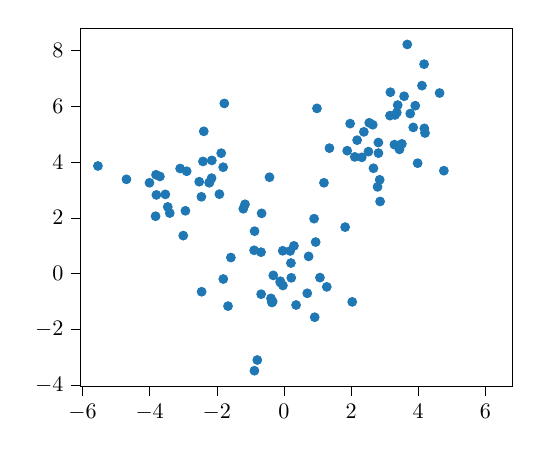
\begin{tikzpicture}[thick,scale=0.8, every node/.style={transform shape}]

\definecolor{color0}{rgb}{0.12156862745098,0.466666666666667,0.705882352941177}

\begin{axis}[
tick align=outside,
tick pos=left,
x grid style={white!69.0196078431373!black},
%xmin=-6.05675528744101, xmax=5.27787573032565,
xmin=-6.05675528744101, xmax=6.80298415266092,
xtick style={color=black},
y grid style={white!69.0196078431373!black},
ymin=-4.05675528744101, ymax=8.80298415266092,
%ymin=-4.06578947588708, ymax=8.80298415266092,
ytick style={color=black}
]
\addplot [only marks, mark=*, draw=color0, fill=color0, colormap/viridis]
table{%
x                      y
-0.358111612392031 -1.03573022195866
2.54059011512305 5.40732724426877
2.64439303639391 5.33779192925331
2.37993615478195 5.08341926202954
-0.108138330543506 -0.272147725049101
-1.66612171369168 -1.16491671279916
1.82276797293495 1.66810423984943
-0.386954794949196 -0.887278921762747
0.297086897817065 0.995913395714418
4.20230143122709 5.04114381567126
4.18098479411033 5.20817168133169
-1.15979760167936 2.48579337246029
-1.21072940472115 2.32564645539021
-1.92310074281666 2.849737736476
-0.794077022732528 -3.09763838394167
-0.879810558070651 -3.48084522004399
0.897589460877768 1.97038397092996
-2.41240086456128 4.0225376563209
-2.14787238675959 4.06031111140356
0.185474121138129 0.813411089586105
0.208319009940496 0.379643070293184
-0.108331721452844 -0.315740368822207
0.915515455672217 -1.56223640998641
0.361160707852192 -1.12526391609712
-2.99962181068817 1.36366577935927
-1.86926540057446 4.31937963197559
1.97167127405905 5.37846226762404
3.38829769446094 6.04358633691308
3.17027424070748 6.50474613140325
2.86412145575591 2.58741981824194
3.57926152941062 6.35979132901094
3.91118505308693 6.02140162936865
0.734555168589413 0.618002625061071
-0.888552360386418 0.837344604908327
-2.93513629393346 2.25270029210883
-2.45909955124887 2.75444952657863
0.982944772711592 5.92494310211316
1.0722787109508 -0.143047009227478
3.76177050379184 5.73921743170339
3.30899718046626 5.68990456424791
3.15857161895561 5.66514809186076
3.36185274192307 5.77406588531824
3.85072378702374 5.2428792846038
4.11118344993143 6.74050825521424
4.63615766530576 6.47510482513503
-0.665776111307205 2.16134751297774
-0.317679888699185 -0.0629296458187575
1.19147659111797 3.25759452658187
-2.45255966188733 -0.649306539777947
-2.38827323869676 5.1019760098924
-3.80990947334099 3.54431506206447
-3.6945185892455 3.48456470113167
-3.09213735335708 3.76910734978884
-1.58108210183386 0.576205666538593
-0.0305854665203686 -0.424590954248704
-0.336311379908108 -0.997344391227889
1.35475062047888 4.49965906131902
1.8835208886715 4.40757117309586
2.66535600163303 3.77813231660804
2.78862863818822 3.11143766434187
2.85133778920804 3.36411834401323
-5.54154478663344 3.85984931952986
0.944278596087085 1.13182749047688
-0.874971110150818 1.52230867430528
-2.52364788757035 3.29543119127435
-2.21841271692549 3.26727594273737
2.03361333854756 -1.01225876863371
-2.89772819748342 3.67099747186657
-2.22758194752147 3.25979487107238
-2.15550016844155 3.42338679220924
3.44185983653917 4.45516210545079
2.51524615285251 4.37419916143041
2.17963557993397 4.78564637341144
2.81220545438285 4.70120393417241
2.10859389528023 4.18592294168646
2.81458938319616 4.32045257984774
3.29006165526776 4.6251028305993
0.218482926894079 -0.149901020185651
2.31841867483311 4.1696634344682
3.51218046217622 4.65210791346245
4.17446946920669 7.5111622752538
-0.430420348837371 3.45705996633102
3.98154238175133 3.96023539287441
-4.00531594259129 3.25737670503793
-4.69073919765948 3.38159404040119
-3.79987123609756 2.82295825942001
-3.53276051991429 2.84153490572953
-3.82369011056774 2.05838460399524
-3.40165671980728 2.17191730886362
-3.46174416837956 2.39161003248653
-1.81022369365007 3.81555936074182
-0.679764120459465 -0.736996202880417
-0.682644108116294 0.76958992767765
0.694353516552503 -0.704212714310419
1.27576879788079 -0.474284940941255
-1.8072024193766 -0.193590780546145
-1.7758920309332 6.10254964560158
-0.0361543454845905 0.819222700941846
3.6731850363502 8.21803989681783
4.76266522951807 3.69025802127189
};
\end{axis}

\end{tikzpicture}

\subcaption{Point cloud $S$.}
\end{center}
\end{subfigure}
\begin{subfigure}[t]{0.49\textwidth}
\begin{center}
% This file was created by tikzplotlib v0.9.2.
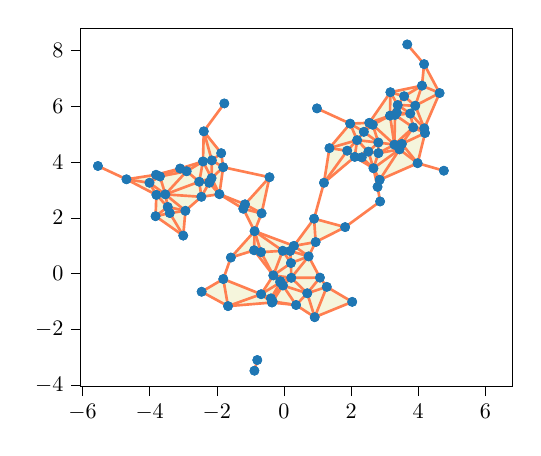
\begin{tikzpicture}[thick,scale=0.8, every node/.style={transform shape}]

\definecolor{color0}{rgb}{0.12156862745098,0.466666666666667,0.705882352941177}
\definecolor{color1}{rgb}{1,0.498039215686275,0.0549019607843137}
\definecolor{color2}{rgb}{0.96078431372549,0.96078431372549,0.862745098039216}
\definecolor{color3}{rgb}{1,0.498039215686275,0.313725490196078}

\begin{axis}[
tick align=outside,
tick pos=left,
x grid style={white!69.0196078431373!black},
%xmin=-6.05675528744101, xmax=5.27787573032565,
xmin=-6.05675528744101, xmax=6.80298415266092,
xtick style={color=black},
y grid style={white!69.0196078431373!black},
ymin=-4.05675528744101, ymax=8.80298415266092,
%ymin=-4.06578947588708, ymax=8.80298415266092,
ytick style={color=black}
]
\addplot [only marks, mark=*, draw=color0, fill=color0, colormap/viridis]
table{%
x                      y
-0.358111612392031 -1.03573022195866
2.54059011512305 5.40732724426877
2.64439303639391 5.33779192925331
2.37993615478195 5.08341926202954
-0.108138330543506 -0.272147725049101
-1.66612171369168 -1.16491671279916
1.82276797293495 1.66810423984943
-0.386954794949196 -0.887278921762747
0.297086897817065 0.995913395714418
4.20230143122709 5.04114381567126
4.18098479411033 5.20817168133169
-1.15979760167936 2.48579337246029
-1.21072940472115 2.32564645539021
-1.92310074281666 2.849737736476
-0.794077022732528 -3.09763838394167
-0.879810558070651 -3.48084522004399
0.897589460877768 1.97038397092996
-2.41240086456128 4.0225376563209
-2.14787238675959 4.06031111140356
0.185474121138129 0.813411089586105
0.208319009940496 0.379643070293184
-0.108331721452844 -0.315740368822207
0.915515455672217 -1.56223640998641
0.361160707852192 -1.12526391609712
-2.99962181068817 1.36366577935927
-1.86926540057446 4.31937963197559
1.97167127405905 5.37846226762404
3.38829769446094 6.04358633691308
3.17027424070748 6.50474613140325
2.86412145575591 2.58741981824194
3.57926152941062 6.35979132901094
3.91118505308693 6.02140162936865
0.734555168589413 0.618002625061071
-0.888552360386418 0.837344604908327
-2.93513629393346 2.25270029210883
-2.45909955124887 2.75444952657863
0.982944772711592 5.92494310211316
1.0722787109508 -0.143047009227478
3.76177050379184 5.73921743170339
3.30899718046626 5.68990456424791
3.15857161895561 5.66514809186076
3.36185274192307 5.77406588531824
3.85072378702374 5.2428792846038
4.11118344993143 6.74050825521424
4.63615766530576 6.47510482513503
-0.665776111307205 2.16134751297774
-0.317679888699185 -0.0629296458187575
1.19147659111797 3.25759452658187
-2.45255966188733 -0.649306539777947
-2.38827323869676 5.1019760098924
-3.80990947334099 3.54431506206447
-3.6945185892455 3.48456470113167
-3.09213735335708 3.76910734978884
-1.58108210183386 0.576205666538593
-0.0305854665203686 -0.424590954248704
-0.336311379908108 -0.997344391227889
1.35475062047888 4.49965906131902
1.8835208886715 4.40757117309586
2.66535600163303 3.77813231660804
2.78862863818822 3.11143766434187
2.85133778920804 3.36411834401323
-5.54154478663344 3.85984931952986
0.944278596087085 1.13182749047688
-0.874971110150818 1.52230867430528
-2.52364788757035 3.29543119127435
-2.21841271692549 3.26727594273737
2.03361333854756 -1.01225876863371
-2.89772819748342 3.67099747186657
-2.22758194752147 3.25979487107238
-2.15550016844155 3.42338679220924
3.44185983653917 4.45516210545079
2.51524615285251 4.37419916143041
2.17963557993397 4.78564637341144
2.81220545438285 4.70120393417241
2.10859389528023 4.18592294168646
2.81458938319616 4.32045257984774
3.29006165526776 4.6251028305993
0.218482926894079 -0.149901020185651
2.31841867483311 4.1696634344682
3.51218046217622 4.65210791346245
4.17446946920669 7.5111622752538
-0.430420348837371 3.45705996633102
3.98154238175133 3.96023539287441
-4.00531594259129 3.25737670503793
-4.69073919765948 3.38159404040119
-3.79987123609756 2.82295825942001
-3.53276051991429 2.84153490572953
-3.82369011056774 2.05838460399524
-3.40165671980728 2.17191730886362
-3.46174416837956 2.39161003248653
-1.81022369365007 3.81555936074182
-0.679764120459465 -0.736996202880417
-0.682644108116294 0.76958992767765
0.694353516552503 -0.704212714310419
1.27576879788079 -0.474284940941255
-1.8072024193766 -0.193590780546145
-1.7758920309332 6.10254964560158
-0.0361543454845905 0.819222700941846
3.6731850363502 8.21803989681783
4.76266522951807 3.69025802127189
};
\path [draw=color2, fill=color2]
(axis cs:-0.358111612392031,-1.03573022195866)
--(axis cs:-0.386954794949196,-0.887278921762747)
--(axis cs:-0.336311379908108,-0.997344391227889)
--cycle;
\path [draw=color2, fill=color2]
(axis cs:3.44185983653917,4.45516210545079)
--(axis cs:3.29006165526776,4.6251028305993)
--(axis cs:3.51218046217622,4.65210791346245)
--cycle;
\path [draw=color2, fill=color2]
(axis cs:-0.108138330543506,-0.272147725049101)
--(axis cs:-0.108331721452844,-0.315740368822207)
--(axis cs:-0.0305854665203686,-0.424590954248704)
--cycle;
\path [draw=color2, fill=color2]
(axis cs:3.30899718046626,5.68990456424791)
--(axis cs:3.15857161895561,5.66514809186076)
--(axis cs:3.36185274192307,5.77406588531824)
--cycle;
\path [draw=color2, fill=color2]
(axis cs:2.54059011512305,5.40732724426877)
--(axis cs:2.64439303639391,5.33779192925331)
--(axis cs:2.37993615478195,5.08341926202954)
--cycle;
\path [draw=color2, fill=color2]
(axis cs:-2.21841271692549,3.26727594273737)
--(axis cs:-2.22758194752147,3.25979487107238)
--(axis cs:-2.15550016844155,3.42338679220924)
--cycle;
\path [draw=color2, fill=color2]
(axis cs:-0.108138330543506,-0.272147725049101)
--(axis cs:-0.0305854665203686,-0.424590954248704)
--(axis cs:0.218482926894079,-0.149901020185651)
--cycle;
\path [draw=color2, fill=color2]
(axis cs:-3.80990947334099,3.54431506206447)
--(axis cs:-3.6945185892455,3.48456470113167)
--(axis cs:-4.00531594259129,3.25737670503793)
--cycle;
\path [draw=color2, fill=color2]
(axis cs:-2.52364788757035,3.29543119127435)
--(axis cs:-2.22758194752147,3.25979487107238)
--(axis cs:-2.15550016844155,3.42338679220924)
--cycle;
\path [draw=color2, fill=color2]
(axis cs:4.20230143122709,5.04114381567126)
--(axis cs:4.18098479411033,5.20817168133169)
--(axis cs:3.85072378702374,5.2428792846038)
--cycle;
\path [draw=color2, fill=color2]
(axis cs:0.297086897817065,0.995913395714418)
--(axis cs:0.185474121138129,0.813411089586105)
--(axis cs:-0.0361543454845905,0.819222700941846)
--cycle;
\path [draw=color2, fill=color2]
(axis cs:2.51524615285251,4.37419916143041)
--(axis cs:2.81220545438285,4.70120393417241)
--(axis cs:2.81458938319616,4.32045257984774)
--cycle;
\path [draw=color2, fill=color2]
(axis cs:-0.108138330543506,-0.272147725049101)
--(axis cs:-0.108331721452844,-0.315740368822207)
--(axis cs:-0.317679888699185,-0.0629296458187575)
--cycle;
\path [draw=color2, fill=color2]
(axis cs:3.38829769446094,6.04358633691308)
--(axis cs:3.76177050379184,5.73921743170339)
--(axis cs:3.36185274192307,5.77406588531824)
--cycle;
\path [draw=color2, fill=color2]
(axis cs:-3.82369011056774,2.05838460399524)
--(axis cs:-3.40165671980728,2.17191730886362)
--(axis cs:-3.46174416837956,2.39161003248653)
--cycle;
\path [draw=color2, fill=color2]
(axis cs:0.185474121138129,0.813411089586105)
--(axis cs:0.208319009940496,0.379643070293184)
--(axis cs:-0.0361543454845905,0.819222700941846)
--cycle;
\path [draw=color2, fill=color2]
(axis cs:3.76177050379184,5.73921743170339)
--(axis cs:3.30899718046626,5.68990456424791)
--(axis cs:3.36185274192307,5.77406588531824)
--cycle;
\path [draw=color2, fill=color2]
(axis cs:-1.92310074281666,2.849737736476)
--(axis cs:-2.21841271692549,3.26727594273737)
--(axis cs:-2.22758194752147,3.25979487107238)
--cycle;
\path [draw=color2, fill=color2]
(axis cs:-2.14787238675959,4.06031111140356)
--(axis cs:-1.86926540057446,4.31937963197559)
--(axis cs:-1.81022369365007,3.81555936074182)
--cycle;
\path [draw=color2, fill=color2]
(axis cs:3.38829769446094,6.04358633691308)
--(axis cs:3.17027424070748,6.50474613140325)
--(axis cs:3.57926152941062,6.35979132901094)
--cycle;
\path [draw=color2, fill=color2]
(axis cs:3.38829769446094,6.04358633691308)
--(axis cs:3.15857161895561,5.66514809186076)
--(axis cs:3.36185274192307,5.77406588531824)
--cycle;
\path [draw=color2, fill=color2]
(axis cs:3.38829769446094,6.04358633691308)
--(axis cs:3.91118505308693,6.02140162936865)
--(axis cs:3.76177050379184,5.73921743170339)
--cycle;
\path [draw=color2, fill=color2]
(axis cs:3.38829769446094,6.04358633691308)
--(axis cs:3.57926152941062,6.35979132901094)
--(axis cs:3.91118505308693,6.02140162936865)
--cycle;
\path [draw=color2, fill=color2]
(axis cs:-2.93513629393346,2.25270029210883)
--(axis cs:-3.40165671980728,2.17191730886362)
--(axis cs:-3.46174416837956,2.39161003248653)
--cycle;
\path [draw=color2, fill=color2]
(axis cs:-3.79987123609756,2.82295825942001)
--(axis cs:-3.53276051991429,2.84153490572953)
--(axis cs:-3.46174416837956,2.39161003248653)
--cycle;
\path [draw=color2, fill=color2]
(axis cs:-0.358111612392031,-1.03573022195866)
--(axis cs:-0.386954794949196,-0.887278921762747)
--(axis cs:-0.679764120459465,-0.736996202880417)
--cycle;
\path [draw=color2, fill=color2]
(axis cs:-2.45909955124887,2.75444952657863)
--(axis cs:-2.52364788757035,3.29543119127435)
--(axis cs:-2.22758194752147,3.25979487107238)
--cycle;
\path [draw=color2, fill=color2]
(axis cs:2.81220545438285,4.70120393417241)
--(axis cs:2.81458938319616,4.32045257984774)
--(axis cs:3.29006165526776,4.6251028305993)
--cycle;
\path [draw=color2, fill=color2]
(axis cs:2.54059011512305,5.40732724426877)
--(axis cs:2.37993615478195,5.08341926202954)
--(axis cs:1.97167127405905,5.37846226762404)
--cycle;
\path [draw=color2, fill=color2]
(axis cs:2.51524615285251,4.37419916143041)
--(axis cs:2.10859389528023,4.18592294168646)
--(axis cs:2.31841867483311,4.1696634344682)
--cycle;
\path [draw=color2, fill=color2]
(axis cs:0.297086897817065,0.995913395714418)
--(axis cs:0.185474121138129,0.813411089586105)
--(axis cs:0.734555168589413,0.618002625061071)
--cycle;
\path [draw=color2, fill=color2]
(axis cs:-1.15979760167936,2.48579337246029)
--(axis cs:-1.21072940472115,2.32564645539021)
--(axis cs:-0.665776111307205,2.16134751297774)
--cycle;
\path [draw=color2, fill=color2]
(axis cs:-0.108138330543506,-0.272147725049101)
--(axis cs:-0.317679888699185,-0.0629296458187575)
--(axis cs:0.218482926894079,-0.149901020185651)
--cycle;
\path [draw=color2, fill=color2]
(axis cs:1.8835208886715,4.40757117309586)
--(axis cs:2.17963557993397,4.78564637341144)
--(axis cs:2.10859389528023,4.18592294168646)
--cycle;
\path [draw=color2, fill=color2]
(axis cs:2.66535600163303,3.77813231660804)
--(axis cs:2.51524615285251,4.37419916143041)
--(axis cs:2.31841867483311,4.1696634344682)
--cycle;
\path [draw=color2, fill=color2]
(axis cs:2.66535600163303,3.77813231660804)
--(axis cs:2.51524615285251,4.37419916143041)
--(axis cs:2.81458938319616,4.32045257984774)
--cycle;
\path [draw=color2, fill=color2]
(axis cs:-1.92310074281666,2.849737736476)
--(axis cs:-2.45909955124887,2.75444952657863)
--(axis cs:-2.22758194752147,3.25979487107238)
--cycle;
\path [draw=color2, fill=color2]
(axis cs:2.51524615285251,4.37419916143041)
--(axis cs:2.17963557993397,4.78564637341144)
--(axis cs:2.10859389528023,4.18592294168646)
--cycle;
\path [draw=color2, fill=color2]
(axis cs:0.185474121138129,0.813411089586105)
--(axis cs:0.208319009940496,0.379643070293184)
--(axis cs:0.734555168589413,0.618002625061071)
--cycle;
\path [draw=color2, fill=color2]
(axis cs:2.37993615478195,5.08341926202954)
--(axis cs:1.97167127405905,5.37846226762404)
--(axis cs:2.17963557993397,4.78564637341144)
--cycle;
\path [draw=color2, fill=color2]
(axis cs:-2.14787238675959,4.06031111140356)
--(axis cs:-2.15550016844155,3.42338679220924)
--(axis cs:-1.81022369365007,3.81555936074182)
--cycle;
\path [draw=color2, fill=color2]
(axis cs:2.37993615478195,5.08341926202954)
--(axis cs:2.17963557993397,4.78564637341144)
--(axis cs:2.81220545438285,4.70120393417241)
--cycle;
\path [draw=color2, fill=color2]
(axis cs:2.51524615285251,4.37419916143041)
--(axis cs:2.17963557993397,4.78564637341144)
--(axis cs:2.81220545438285,4.70120393417241)
--cycle;
\path [draw=color2, fill=color2]
(axis cs:3.44185983653917,4.45516210545079)
--(axis cs:2.81458938319616,4.32045257984774)
--(axis cs:3.29006165526776,4.6251028305993)
--cycle;
\path [draw=color2, fill=color2]
(axis cs:-2.41240086456128,4.0225376563209)
--(axis cs:-2.14787238675959,4.06031111140356)
--(axis cs:-2.15550016844155,3.42338679220924)
--cycle;
\path [draw=color2, fill=color2]
(axis cs:2.64439303639391,5.33779192925331)
--(axis cs:2.37993615478195,5.08341926202954)
--(axis cs:2.81220545438285,4.70120393417241)
--cycle;
\path [draw=color2, fill=color2]
(axis cs:-0.386954794949196,-0.887278921762747)
--(axis cs:-0.108331721452844,-0.315740368822207)
--(axis cs:-0.0305854665203686,-0.424590954248704)
--cycle;
\path [draw=color2, fill=color2]
(axis cs:-4.00531594259129,3.25737670503793)
--(axis cs:-3.79987123609756,2.82295825942001)
--(axis cs:-3.53276051991429,2.84153490572953)
--cycle;
\path [draw=color2, fill=color2]
(axis cs:-3.6945185892455,3.48456470113167)
--(axis cs:-4.00531594259129,3.25737670503793)
--(axis cs:-3.53276051991429,2.84153490572953)
--cycle;
\path [draw=color2, fill=color2]
(axis cs:1.0722787109508,-0.143047009227478)
--(axis cs:0.694353516552503,-0.704212714310419)
--(axis cs:1.27576879788079,-0.474284940941255)
--cycle;
\path [draw=color2, fill=color2]
(axis cs:0.297086897817065,0.995913395714418)
--(axis cs:0.734555168589413,0.618002625061071)
--(axis cs:0.944278596087085,1.13182749047688)
--cycle;
\path [draw=color2, fill=color2]
(axis cs:0.208319009940496,0.379643070293184)
--(axis cs:-0.317679888699185,-0.0629296458187575)
--(axis cs:0.218482926894079,-0.149901020185651)
--cycle;
\path [draw=color2, fill=color2]
(axis cs:3.76177050379184,5.73921743170339)
--(axis cs:3.30899718046626,5.68990456424791)
--(axis cs:3.85072378702374,5.2428792846038)
--cycle;
\path [draw=color2, fill=color2]
(axis cs:4.18098479411033,5.20817168133169)
--(axis cs:3.76177050379184,5.73921743170339)
--(axis cs:3.85072378702374,5.2428792846038)
--cycle;
\path [draw=color2, fill=color2]
(axis cs:-0.386954794949196,-0.887278921762747)
--(axis cs:-0.108331721452844,-0.315740368822207)
--(axis cs:-0.679764120459465,-0.736996202880417)
--cycle;
\path [draw=color2, fill=color2]
(axis cs:2.54059011512305,5.40732724426877)
--(axis cs:2.64439303639391,5.33779192925331)
--(axis cs:3.15857161895561,5.66514809186076)
--cycle;
\path [draw=color2, fill=color2]
(axis cs:-0.386954794949196,-0.887278921762747)
--(axis cs:-0.0305854665203686,-0.424590954248704)
--(axis cs:-0.336311379908108,-0.997344391227889)
--cycle;
\path [draw=color2, fill=color2]
(axis cs:-1.92310074281666,2.849737736476)
--(axis cs:-2.21841271692549,3.26727594273737)
--(axis cs:-2.15550016844155,3.42338679220924)
--cycle;
\path [draw=color2, fill=color2]
(axis cs:-2.41240086456128,4.0225376563209)
--(axis cs:-2.52364788757035,3.29543119127435)
--(axis cs:-2.15550016844155,3.42338679220924)
--cycle;
\path [draw=color2, fill=color2]
(axis cs:-2.41240086456128,4.0225376563209)
--(axis cs:-2.52364788757035,3.29543119127435)
--(axis cs:-2.89772819748342,3.67099747186657)
--cycle;
\path [draw=color2, fill=color2]
(axis cs:3.57926152941062,6.35979132901094)
--(axis cs:3.91118505308693,6.02140162936865)
--(axis cs:4.11118344993143,6.74050825521424)
--cycle;
\path [draw=color2, fill=color2]
(axis cs:-0.108331721452844,-0.315740368822207)
--(axis cs:-0.317679888699185,-0.0629296458187575)
--(axis cs:-0.679764120459465,-0.736996202880417)
--cycle;
\path [draw=color2, fill=color2]
(axis cs:-3.79987123609756,2.82295825942001)
--(axis cs:-3.82369011056774,2.05838460399524)
--(axis cs:-3.46174416837956,2.39161003248653)
--cycle;
\path [draw=color2, fill=color2]
(axis cs:-0.358111612392031,-1.03573022195866)
--(axis cs:0.361160707852192,-1.12526391609712)
--(axis cs:-0.336311379908108,-0.997344391227889)
--cycle;
\path [draw=color2, fill=color2]
(axis cs:-0.0305854665203686,-0.424590954248704)
--(axis cs:0.218482926894079,-0.149901020185651)
--(axis cs:0.694353516552503,-0.704212714310419)
--cycle;
\path [draw=color2, fill=color2]
(axis cs:4.20230143122709,5.04114381567126)
--(axis cs:3.85072378702374,5.2428792846038)
--(axis cs:3.51218046217622,4.65210791346245)
--cycle;
\path [draw=color2, fill=color2]
(axis cs:-0.888552360386418,0.837344604908327)
--(axis cs:-0.874971110150818,1.52230867430528)
--(axis cs:-0.682644108116294,0.76958992767765)
--cycle;
\path [draw=color2, fill=color2]
(axis cs:-2.41240086456128,4.0225376563209)
--(axis cs:-3.09213735335708,3.76910734978884)
--(axis cs:-2.89772819748342,3.67099747186657)
--cycle;
\path [draw=color2, fill=color2]
(axis cs:0.361160707852192,-1.12526391609712)
--(axis cs:-0.0305854665203686,-0.424590954248704)
--(axis cs:0.694353516552503,-0.704212714310419)
--cycle;
\path [draw=color2, fill=color2]
(axis cs:0.361160707852192,-1.12526391609712)
--(axis cs:-0.0305854665203686,-0.424590954248704)
--(axis cs:-0.336311379908108,-0.997344391227889)
--cycle;
\path [draw=color2, fill=color2]
(axis cs:-1.21072940472115,2.32564645539021)
--(axis cs:-0.665776111307205,2.16134751297774)
--(axis cs:-0.874971110150818,1.52230867430528)
--cycle;
\path [draw=color2, fill=color2]
(axis cs:3.91118505308693,6.02140162936865)
--(axis cs:4.11118344993143,6.74050825521424)
--(axis cs:4.63615766530576,6.47510482513503)
--cycle;
\path [draw=color2, fill=color2]
(axis cs:1.0722787109508,-0.143047009227478)
--(axis cs:0.218482926894079,-0.149901020185651)
--(axis cs:0.694353516552503,-0.704212714310419)
--cycle;
\path [draw=color2, fill=color2]
(axis cs:0.915515455672217,-1.56223640998641)
--(axis cs:0.361160707852192,-1.12526391609712)
--(axis cs:0.694353516552503,-0.704212714310419)
--cycle;
\path [draw=color2, fill=color2]
(axis cs:-1.15979760167936,2.48579337246029)
--(axis cs:-1.21072940472115,2.32564645539021)
--(axis cs:-1.92310074281666,2.849737736476)
--cycle;
\path [draw=color2, fill=color2]
(axis cs:3.44185983653917,4.45516210545079)
--(axis cs:3.51218046217622,4.65210791346245)
--(axis cs:3.98154238175133,3.96023539287441)
--cycle;
\path [draw=color2, fill=color2]
(axis cs:-2.93513629393346,2.25270029210883)
--(axis cs:-3.53276051991429,2.84153490572953)
--(axis cs:-3.46174416837956,2.39161003248653)
--cycle;
\path [draw=color2, fill=color2]
(axis cs:-2.99962181068817,1.36366577935927)
--(axis cs:-2.93513629393346,2.25270029210883)
--(axis cs:-3.40165671980728,2.17191730886362)
--cycle;
\path [draw=color2, fill=color2]
(axis cs:4.18098479411033,5.20817168133169)
--(axis cs:3.91118505308693,6.02140162936865)
--(axis cs:3.76177050379184,5.73921743170339)
--cycle;
\path [draw=color2, fill=color2]
(axis cs:0.208319009940496,0.379643070293184)
--(axis cs:-0.317679888699185,-0.0629296458187575)
--(axis cs:-0.0361543454845905,0.819222700941846)
--cycle;
\path [draw=color2, fill=color2]
(axis cs:-3.80990947334099,3.54431506206447)
--(axis cs:-3.6945185892455,3.48456470113167)
--(axis cs:-3.09213735335708,3.76910734978884)
--cycle;
\path [draw=color2, fill=color2]
(axis cs:-3.80990947334099,3.54431506206447)
--(axis cs:-4.00531594259129,3.25737670503793)
--(axis cs:-4.69073919765948,3.38159404040119)
--cycle;
\path [draw=color2, fill=color2]
(axis cs:-0.317679888699185,-0.0629296458187575)
--(axis cs:-0.682644108116294,0.76958992767765)
--(axis cs:-0.0361543454845905,0.819222700941846)
--cycle;
\path [draw=color2, fill=color2]
(axis cs:1.35475062047888,4.49965906131902)
--(axis cs:1.8835208886715,4.40757117309586)
--(axis cs:2.17963557993397,4.78564637341144)
--cycle;
\path [draw=color2, fill=color2]
(axis cs:2.66535600163303,3.77813231660804)
--(axis cs:2.10859389528023,4.18592294168646)
--(axis cs:2.31841867483311,4.1696634344682)
--cycle;
\path [draw=color2, fill=color2]
(axis cs:3.38829769446094,6.04358633691308)
--(axis cs:3.17027424070748,6.50474613140325)
--(axis cs:3.15857161895561,5.66514809186076)
--cycle;
\path [draw=color2, fill=color2]
(axis cs:0.208319009940496,0.379643070293184)
--(axis cs:0.734555168589413,0.618002625061071)
--(axis cs:0.218482926894079,-0.149901020185651)
--cycle;
\path [draw=color2, fill=color2]
(axis cs:0.734555168589413,0.618002625061071)
--(axis cs:1.0722787109508,-0.143047009227478)
--(axis cs:0.218482926894079,-0.149901020185651)
--cycle;
\path [draw=color2, fill=color2]
(axis cs:-3.6945185892455,3.48456470113167)
--(axis cs:-3.09213735335708,3.76910734978884)
--(axis cs:-2.89772819748342,3.67099747186657)
--cycle;
\path [draw=color2, fill=color2]
(axis cs:3.85072378702374,5.2428792846038)
--(axis cs:3.29006165526776,4.6251028305993)
--(axis cs:3.51218046217622,4.65210791346245)
--cycle;
\path [draw=color2, fill=color2]
(axis cs:-3.6945185892455,3.48456470113167)
--(axis cs:-2.89772819748342,3.67099747186657)
--(axis cs:-3.53276051991429,2.84153490572953)
--cycle;
\path [draw=color2, fill=color2]
(axis cs:2.64439303639391,5.33779192925331)
--(axis cs:2.81220545438285,4.70120393417241)
--(axis cs:3.29006165526776,4.6251028305993)
--cycle;
\path [draw=color2, fill=color2]
(axis cs:-1.66612171369168,-1.16491671279916)
--(axis cs:-2.45255966188733,-0.649306539777947)
--(axis cs:-1.8072024193766,-0.193590780546145)
--cycle;
\path [draw=color2, fill=color2]
(axis cs:2.64439303639391,5.33779192925331)
--(axis cs:3.15857161895561,5.66514809186076)
--(axis cs:3.29006165526776,4.6251028305993)
--cycle;
\path [draw=color2, fill=color2]
(axis cs:3.30899718046626,5.68990456424791)
--(axis cs:3.15857161895561,5.66514809186076)
--(axis cs:3.29006165526776,4.6251028305993)
--cycle;
\path [draw=color2, fill=color2]
(axis cs:3.30899718046626,5.68990456424791)
--(axis cs:3.85072378702374,5.2428792846038)
--(axis cs:3.29006165526776,4.6251028305993)
--cycle;
\path [draw=color2, fill=color2]
(axis cs:1.97167127405905,5.37846226762404)
--(axis cs:1.35475062047888,4.49965906131902)
--(axis cs:2.17963557993397,4.78564637341144)
--cycle;
\path [draw=color2, fill=color2]
(axis cs:-2.93513629393346,2.25270029210883)
--(axis cs:-2.45909955124887,2.75444952657863)
--(axis cs:-3.53276051991429,2.84153490572953)
--cycle;
\path [draw=color2, fill=color2]
(axis cs:-2.14787238675959,4.06031111140356)
--(axis cs:-1.86926540057446,4.31937963197559)
--(axis cs:-2.38827323869676,5.1019760098924)
--cycle;
\path [draw=color2, fill=color2]
(axis cs:-2.41240086456128,4.0225376563209)
--(axis cs:-2.14787238675959,4.06031111140356)
--(axis cs:-2.38827323869676,5.1019760098924)
--cycle;
\path [draw=color2, fill=color2]
(axis cs:-1.92310074281666,2.849737736476)
--(axis cs:-2.15550016844155,3.42338679220924)
--(axis cs:-1.81022369365007,3.81555936074182)
--cycle;
\path [draw=color2, fill=color2]
(axis cs:2.66535600163303,3.77813231660804)
--(axis cs:2.78862863818822,3.11143766434187)
--(axis cs:2.85133778920804,3.36411834401323)
--cycle;
\path [draw=color2, fill=color2]
(axis cs:-2.99962181068817,1.36366577935927)
--(axis cs:-3.82369011056774,2.05838460399524)
--(axis cs:-3.40165671980728,2.17191730886362)
--cycle;
\path [draw=color2, fill=color2]
(axis cs:1.82276797293495,1.66810423984943)
--(axis cs:0.897589460877768,1.97038397092996)
--(axis cs:0.944278596087085,1.13182749047688)
--cycle;
\path [draw=color2, fill=color2]
(axis cs:4.20230143122709,5.04114381567126)
--(axis cs:3.51218046217622,4.65210791346245)
--(axis cs:3.98154238175133,3.96023539287441)
--cycle;
\path [draw=color2, fill=color2]
(axis cs:-0.874971110150818,1.52230867430528)
--(axis cs:-0.682644108116294,0.76958992767765)
--(axis cs:-0.0361543454845905,0.819222700941846)
--cycle;
\path [draw=color2, fill=color2]
(axis cs:-2.52364788757035,3.29543119127435)
--(axis cs:-2.89772819748342,3.67099747186657)
--(axis cs:-3.53276051991429,2.84153490572953)
--cycle;
\path [draw=color2, fill=color2]
(axis cs:-2.45909955124887,2.75444952657863)
--(axis cs:-2.52364788757035,3.29543119127435)
--(axis cs:-3.53276051991429,2.84153490572953)
--cycle;
\path [draw=color2, fill=color2]
(axis cs:0.915515455672217,-1.56223640998641)
--(axis cs:0.694353516552503,-0.704212714310419)
--(axis cs:1.27576879788079,-0.474284940941255)
--cycle;
\path [draw=color2, fill=color2]
(axis cs:0.297086897817065,0.995913395714418)
--(axis cs:0.897589460877768,1.97038397092996)
--(axis cs:0.944278596087085,1.13182749047688)
--cycle;
\path [draw=color2, fill=color2]
(axis cs:2.66535600163303,3.77813231660804)
--(axis cs:3.44185983653917,4.45516210545079)
--(axis cs:2.81458938319616,4.32045257984774)
--cycle;
\path [draw=color2, fill=color2]
(axis cs:3.17027424070748,6.50474613140325)
--(axis cs:3.57926152941062,6.35979132901094)
--(axis cs:4.11118344993143,6.74050825521424)
--cycle;
\path [draw=color2, fill=color2]
(axis cs:4.11118344993143,6.74050825521424)
--(axis cs:4.63615766530576,6.47510482513503)
--(axis cs:4.17446946920669,7.5111622752538)
--cycle;
\path [draw=color2, fill=color2]
(axis cs:-0.888552360386418,0.837344604908327)
--(axis cs:-1.58108210183386,0.576205666538593)
--(axis cs:-0.874971110150818,1.52230867430528)
--cycle;
\path [draw=color2, fill=color2]
(axis cs:-4.00531594259129,3.25737670503793)
--(axis cs:-4.69073919765948,3.38159404040119)
--(axis cs:-3.79987123609756,2.82295825942001)
--cycle;
\path [draw=color2, fill=color2]
(axis cs:2.66535600163303,3.77813231660804)
--(axis cs:2.85133778920804,3.36411834401323)
--(axis cs:3.44185983653917,4.45516210545079)
--cycle;
\path [draw=color2, fill=color2]
(axis cs:-1.66612171369168,-1.16491671279916)
--(axis cs:-0.679764120459465,-0.736996202880417)
--(axis cs:-1.8072024193766,-0.193590780546145)
--cycle;
\path [draw=color2, fill=color2]
(axis cs:0.915515455672217,-1.56223640998641)
--(axis cs:2.03361333854756,-1.01225876863371)
--(axis cs:1.27576879788079,-0.474284940941255)
--cycle;
\path [draw=color2, fill=color2]
(axis cs:2.85133778920804,3.36411834401323)
--(axis cs:3.44185983653917,4.45516210545079)
--(axis cs:3.98154238175133,3.96023539287441)
--cycle;
\path [draw=color2, fill=color2]
(axis cs:-1.15979760167936,2.48579337246029)
--(axis cs:-0.665776111307205,2.16134751297774)
--(axis cs:-0.430420348837371,3.45705996633102)
--cycle;
\path [draw=color2, fill=color2]
(axis cs:1.19147659111797,3.25759452658187)
--(axis cs:1.8835208886715,4.40757117309586)
--(axis cs:2.10859389528023,4.18592294168646)
--cycle;
\path [draw=color2, fill=color2]
(axis cs:1.19147659111797,3.25759452658187)
--(axis cs:1.35475062047888,4.49965906131902)
--(axis cs:1.8835208886715,4.40757117309586)
--cycle;
\path [draw=color2, fill=color2]
(axis cs:2.54059011512305,5.40732724426877)
--(axis cs:3.17027424070748,6.50474613140325)
--(axis cs:3.15857161895561,5.66514809186076)
--cycle;
\path [draw=color2, fill=color2]
(axis cs:4.18098479411033,5.20817168133169)
--(axis cs:3.91118505308693,6.02140162936865)
--(axis cs:4.63615766530576,6.47510482513503)
--cycle;
\path [draw=color2, fill=color2]
(axis cs:0.297086897817065,0.995913395714418)
--(axis cs:-0.874971110150818,1.52230867430528)
--(axis cs:-0.0361543454845905,0.819222700941846)
--cycle;
\path [draw=color2, fill=color2]
(axis cs:-0.888552360386418,0.837344604908327)
--(axis cs:-0.317679888699185,-0.0629296458187575)
--(axis cs:-0.682644108116294,0.76958992767765)
--cycle;
\path [draw=color2, fill=color2]
(axis cs:-0.358111612392031,-1.03573022195866)
--(axis cs:-1.66612171369168,-1.16491671279916)
--(axis cs:-0.679764120459465,-0.736996202880417)
--cycle;
\addplot [very thick, color3]
table {%
-2.21841271692549 3.26727594273737
-2.22758194752147 3.25979487107238
};
\addplot [very thick, color3]
table {%
-0.108138330543506 -0.272147725049101
-0.108331721452844 -0.315740368822207
};
\addplot [very thick, color3]
table {%
-0.358111612392031 -1.03573022195866
-0.336311379908108 -0.997344391227889
};
\addplot [very thick, color3]
table {%
3.30899718046626 5.68990456424791
3.36185274192307 5.77406588531824
};
\addplot [very thick, color3]
table {%
-0.386954794949196 -0.887278921762747
-0.336311379908108 -0.997344391227889
};
\addplot [very thick, color3]
table {%
2.54059011512305 5.40732724426877
2.64439303639391 5.33779192925331
};
\addplot [very thick, color3]
table {%
-3.80990947334099 3.54431506206447
-3.6945185892455 3.48456470113167
};
\addplot [very thick, color3]
table {%
-0.108331721452844 -0.315740368822207
-0.0305854665203686 -0.424590954248704
};
\addplot [very thick, color3]
table {%
3.30899718046626 5.68990456424791
3.15857161895561 5.66514809186076
};
\addplot [very thick, color3]
table {%
-1.15979760167936 2.48579337246029
-1.21072940472115 2.32564645539021
};
\addplot [very thick, color3]
table {%
-2.21841271692549 3.26727594273737
-2.15550016844155 3.42338679220924
};
\addplot [very thick, color3]
table {%
4.20230143122709 5.04114381567126
4.18098479411033 5.20817168133169
};
\addplot [very thick, color3]
table {%
-0.358111612392031 -1.03573022195866
-0.386954794949196 -0.887278921762747
};
\addplot [very thick, color3]
table {%
3.44185983653917 4.45516210545079
3.51218046217622 4.65210791346245
};
\addplot [very thick, color3]
table {%
2.10859389528023 4.18592294168646
2.31841867483311 4.1696634344682
};
\addplot [very thick, color3]
table {%
0.297086897817065 0.995913395714418
0.185474121138129 0.813411089586105
};
\addplot [very thick, color3]
table {%
-0.888552360386418 0.837344604908327
-0.682644108116294 0.76958992767765
};
\addplot [very thick, color3]
table {%
-3.09213735335708 3.76910734978884
-2.89772819748342 3.67099747186657
};
\addplot [very thick, color3]
table {%
0.185474121138129 0.813411089586105
-0.0361543454845905 0.819222700941846
};
\addplot [very thick, color3]
table {%
3.29006165526776 4.6251028305993
3.51218046217622 4.65210791346245
};
\addplot [very thick, color3]
table {%
-3.40165671980728 2.17191730886362
-3.46174416837956 2.39161003248653
};
\addplot [very thick, color3]
table {%
3.44185983653917 4.45516210545079
3.29006165526776 4.6251028305993
};
\addplot [very thick, color3]
table {%
2.78862863818822 3.11143766434187
2.85133778920804 3.36411834401323
};
\addplot [very thick, color3]
table {%
-2.41240086456128 4.0225376563209
-2.14787238675959 4.06031111140356
};
\addplot [very thick, color3]
table {%
-3.79987123609756 2.82295825942001
-3.53276051991429 2.84153490572953
};
\addplot [very thick, color3]
table {%
3.38829769446094 6.04358633691308
3.36185274192307 5.77406588531824
};
\addplot [very thick, color3]
table {%
2.51524615285251 4.37419916143041
2.31841867483311 4.1696634344682
};
\addplot [very thick, color3]
table {%
-0.108138330543506 -0.272147725049101
-0.0305854665203686 -0.424590954248704
};
\addplot [very thick, color3]
table {%
-0.108138330543506 -0.272147725049101
-0.317679888699185 -0.0629296458187575
};
\addplot [very thick, color3]
table {%
-2.52364788757035 3.29543119127435
-2.22758194752147 3.25979487107238
};
\addplot [very thick, color3]
table {%
2.51524615285251 4.37419916143041
2.81458938319616 4.32045257984774
};
\addplot [very thick, color3]
table {%
3.15857161895561 5.66514809186076
3.36185274192307 5.77406588531824
};
\addplot [very thick, color3]
table {%
1.8835208886715 4.40757117309586
2.10859389528023 4.18592294168646
};
\addplot [very thick, color3]
table {%
3.91118505308693 6.02140162936865
3.76177050379184 5.73921743170339
};
\addplot [very thick, color3]
table {%
-0.386954794949196 -0.887278921762747
-0.679764120459465 -0.736996202880417
};
\addplot [very thick, color3]
table {%
4.18098479411033 5.20817168133169
3.85072378702374 5.2428792846038
};
\addplot [very thick, color3]
table {%
-3.80990947334099 3.54431506206447
-4.00531594259129 3.25737670503793
};
\addplot [very thick, color3]
table {%
-0.108138330543506 -0.272147725049101
0.218482926894079 -0.149901020185651
};
\addplot [very thick, color3]
table {%
2.37993615478195 5.08341926202954
2.17963557993397 4.78564637341144
};
\addplot [very thick, color3]
table {%
2.54059011512305 5.40732724426877
2.37993615478195 5.08341926202954
};
\addplot [very thick, color3]
table {%
2.64439303639391 5.33779192925331
2.37993615478195 5.08341926202954
};
\addplot [very thick, color3]
table {%
3.38829769446094 6.04358633691308
3.57926152941062 6.35979132901094
};
\addplot [very thick, color3]
table {%
-2.22758194752147 3.25979487107238
-2.15550016844155 3.42338679220924
};
\addplot [very thick, color3]
table {%
-0.0305854665203686 -0.424590954248704
0.218482926894079 -0.149901020185651
};
\addplot [very thick, color3]
table {%
-2.14787238675959 4.06031111140356
-1.86926540057446 4.31937963197559
};
\addplot [very thick, color3]
table {%
2.81220545438285 4.70120393417241
2.81458938319616 4.32045257984774
};
\addplot [very thick, color3]
table {%
-3.6945185892455 3.48456470113167
-4.00531594259129 3.25737670503793
};
\addplot [very thick, color3]
table {%
1.0722787109508 -0.143047009227478
1.27576879788079 -0.474284940941255
};
\addplot [very thick, color3]
table {%
-0.794077022732528 -3.09763838394167
-0.879810558070651 -3.48084522004399
};
\addplot [very thick, color3]
table {%
3.76177050379184 5.73921743170339
3.36185274192307 5.77406588531824
};
\addplot [very thick, color3]
table {%
-2.52364788757035 3.29543119127435
-2.15550016844155 3.42338679220924
};
\addplot [very thick, color3]
table {%
4.20230143122709 5.04114381567126
3.85072378702374 5.2428792846038
};
\addplot [very thick, color3]
table {%
-2.14787238675959 4.06031111140356
-1.81022369365007 3.81555936074182
};
\addplot [very thick, color3]
table {%
3.17027424070748 6.50474613140325
3.57926152941062 6.35979132901094
};
\addplot [very thick, color3]
table {%
0.185474121138129 0.813411089586105
0.208319009940496 0.379643070293184
};
\addplot [very thick, color3]
table {%
0.297086897817065 0.995913395714418
-0.0361543454845905 0.819222700941846
};
\addplot [very thick, color3]
table {%
-3.82369011056774 2.05838460399524
-3.40165671980728 2.17191730886362
};
\addplot [very thick, color3]
table {%
2.51524615285251 4.37419916143041
2.81220545438285 4.70120393417241
};
\addplot [very thick, color3]
table {%
2.66535600163303 3.77813231660804
2.85133778920804 3.36411834401323
};
\addplot [very thick, color3]
table {%
-3.53276051991429 2.84153490572953
-3.46174416837956 2.39161003248653
};
\addplot [very thick, color3]
table {%
-0.108331721452844 -0.315740368822207
-0.317679888699185 -0.0629296458187575
};
\addplot [very thick, color3]
table {%
-2.93513629393346 2.25270029210883
-3.40165671980728 2.17191730886362
};
\addplot [very thick, color3]
table {%
3.57926152941062 6.35979132901094
3.91118505308693 6.02140162936865
};
\addplot [very thick, color3]
table {%
1.8835208886715 4.40757117309586
2.17963557993397 4.78564637341144
};
\addplot [very thick, color3]
table {%
-4.00531594259129 3.25737670503793
-3.79987123609756 2.82295825942001
};
\addplot [very thick, color3]
table {%
3.38829769446094 6.04358633691308
3.76177050379184 5.73921743170339
};
\addplot [very thick, color3]
table {%
2.81220545438285 4.70120393417241
3.29006165526776 4.6251028305993
};
\addplot [very thick, color3]
table {%
-3.82369011056774 2.05838460399524
-3.46174416837956 2.39161003248653
};
\addplot [very thick, color3]
table {%
2.37993615478195 5.08341926202954
1.97167127405905 5.37846226762404
};
\addplot [very thick, color3]
table {%
3.76177050379184 5.73921743170339
3.85072378702374 5.2428792846038
};
\addplot [very thick, color3]
table {%
0.208319009940496 0.379643070293184
-0.0361543454845905 0.819222700941846
};
\addplot [very thick, color3]
table {%
-1.86926540057446 4.31937963197559
-1.81022369365007 3.81555936074182
};
\addplot [very thick, color3]
table {%
3.38829769446094 6.04358633691308
3.17027424070748 6.50474613140325
};
\addplot [very thick, color3]
table {%
-1.92310074281666 2.849737736476
-2.22758194752147 3.25979487107238
};
\addplot [very thick, color3]
table {%
3.76177050379184 5.73921743170339
3.30899718046626 5.68990456424791
};
\addplot [very thick, color3]
table {%
-1.92310074281666 2.849737736476
-2.21841271692549 3.26727594273737
};
\addplot [very thick, color3]
table {%
-2.15550016844155 3.42338679220924
-1.81022369365007 3.81555936074182
};
\addplot [very thick, color3]
table {%
2.66535600163303 3.77813231660804
2.31841867483311 4.1696634344682
};
\addplot [very thick, color3]
table {%
3.38829769446094 6.04358633691308
3.91118505308693 6.02140162936865
};
\addplot [very thick, color3]
table {%
2.86412145575591 2.58741981824194
2.78862863818822 3.11143766434187
};
\addplot [very thick, color3]
table {%
0.208319009940496 0.379643070293184
0.218482926894079 -0.149901020185651
};
\addplot [very thick, color3]
table {%
-2.52364788757035 3.29543119127435
-2.89772819748342 3.67099747186657
};
\addplot [very thick, color3]
table {%
2.51524615285251 4.37419916143041
2.17963557993397 4.78564637341144
};
\addplot [very thick, color3]
table {%
3.38829769446094 6.04358633691308
3.15857161895561 5.66514809186076
};
\addplot [very thick, color3]
table {%
1.35475062047888 4.49965906131902
1.8835208886715 4.40757117309586
};
\addplot [very thick, color3]
table {%
0.361160707852192 -1.12526391609712
0.694353516552503 -0.704212714310419
};
\addplot [very thick, color3]
table {%
-1.92310074281666 2.849737736476
-2.45909955124887 2.75444952657863
};
\addplot [very thick, color3]
table {%
-2.45909955124887 2.75444952657863
-2.52364788757035 3.29543119127435
};
\addplot [very thick, color3]
table {%
-2.93513629393346 2.25270029210883
-3.46174416837956 2.39161003248653
};
\addplot [very thick, color3]
table {%
-3.79987123609756 2.82295825942001
-3.46174416837956 2.39161003248653
};
\addplot [very thick, color3]
table {%
0.734555168589413 0.618002625061071
0.944278596087085 1.13182749047688
};
\addplot [very thick, color3]
table {%
-2.45909955124887 2.75444952657863
-2.22758194752147 3.25979487107238
};
\addplot [very thick, color3]
table {%
-0.358111612392031 -1.03573022195866
-0.679764120459465 -0.736996202880417
};
\addplot [very thick, color3]
table {%
2.66535600163303 3.77813231660804
2.81458938319616 4.32045257984774
};
\addplot [very thick, color3]
table {%
2.81458938319616 4.32045257984774
3.29006165526776 4.6251028305993
};
\addplot [very thick, color3]
table {%
-1.21072940472115 2.32564645539021
-0.665776111307205 2.16134751297774
};
\addplot [very thick, color3]
table {%
2.54059011512305 5.40732724426877
1.97167127405905 5.37846226762404
};
\addplot [very thick, color3]
table {%
2.37993615478195 5.08341926202954
2.81220545438285 4.70120393417241
};
\addplot [very thick, color3]
table {%
0.208319009940496 0.379643070293184
0.734555168589413 0.618002625061071
};
\addplot [very thick, color3]
table {%
0.297086897817065 0.995913395714418
0.734555168589413 0.618002625061071
};
\addplot [very thick, color3]
table {%
2.51524615285251 4.37419916143041
2.10859389528023 4.18592294168646
};
\addplot [very thick, color3]
table {%
0.185474121138129 0.813411089586105
0.734555168589413 0.618002625061071
};
\addplot [very thick, color3]
table {%
-0.386954794949196 -0.887278921762747
-0.0305854665203686 -0.424590954248704
};
\addplot [very thick, color3]
table {%
4.11118344993143 6.74050825521424
4.63615766530576 6.47510482513503
};
\addplot [very thick, color3]
table {%
-1.15979760167936 2.48579337246029
-0.665776111307205 2.16134751297774
};
\addplot [very thick, color3]
table {%
-0.317679888699185 -0.0629296458187575
0.218482926894079 -0.149901020185651
};
\addplot [very thick, color3]
table {%
-2.41240086456128 4.0225376563209
-2.89772819748342 3.67099747186657
};
\addplot [very thick, color3]
table {%
2.17963557993397 4.78564637341144
2.10859389528023 4.18592294168646
};
\addplot [very thick, color3]
table {%
2.64439303639391 5.33779192925331
3.15857161895561 5.66514809186076
};
\addplot [very thick, color3]
table {%
2.66535600163303 3.77813231660804
2.51524615285251 4.37419916143041
};
\addplot [very thick, color3]
table {%
0.694353516552503 -0.704212714310419
1.27576879788079 -0.474284940941255
};
\addplot [very thick, color3]
table {%
1.97167127405905 5.37846226762404
2.17963557993397 4.78564637341144
};
\addplot [very thick, color3]
table {%
-2.14787238675959 4.06031111140356
-2.15550016844155 3.42338679220924
};
\addplot [very thick, color3]
table {%
2.17963557993397 4.78564637341144
2.81220545438285 4.70120393417241
};
\addplot [very thick, color3]
table {%
-0.682644108116294 0.76958992767765
-0.0361543454845905 0.819222700941846
};
\addplot [very thick, color3]
table {%
3.44185983653917 4.45516210545079
2.81458938319616 4.32045257984774
};
\addplot [very thick, color3]
table {%
-2.41240086456128 4.0225376563209
-2.15550016844155 3.42338679220924
};
\addplot [very thick, color3]
table {%
3.57926152941062 6.35979132901094
4.11118344993143 6.74050825521424
};
\addplot [very thick, color3]
table {%
2.64439303639391 5.33779192925331
2.81220545438285 4.70120393417241
};
\addplot [very thick, color3]
table {%
0.297086897817065 0.995913395714418
0.944278596087085 1.13182749047688
};
\addplot [very thick, color3]
table {%
-3.6945185892455 3.48456470113167
-3.53276051991429 2.84153490572953
};
\addplot [very thick, color3]
table {%
-0.386954794949196 -0.887278921762747
-0.108331721452844 -0.315740368822207
};
\addplot [very thick, color3]
table {%
-3.6945185892455 3.48456470113167
-3.09213735335708 3.76910734978884
};
\addplot [very thick, color3]
table {%
-0.665776111307205 2.16134751297774
-0.874971110150818 1.52230867430528
};
\addplot [very thick, color3]
table {%
-4.00531594259129 3.25737670503793
-3.53276051991429 2.84153490572953
};
\addplot [very thick, color3]
table {%
1.0722787109508 -0.143047009227478
0.694353516552503 -0.704212714310419
};
\addplot [very thick, color3]
table {%
3.85072378702374 5.2428792846038
3.51218046217622 4.65210791346245
};
\addplot [very thick, color3]
table {%
-0.888552360386418 0.837344604908327
-0.874971110150818 1.52230867430528
};
\addplot [very thick, color3]
table {%
0.208319009940496 0.379643070293184
-0.317679888699185 -0.0629296458187575
};
\addplot [very thick, color3]
table {%
-2.93513629393346 2.25270029210883
-2.45909955124887 2.75444952657863
};
\addplot [very thick, color3]
table {%
-4.00531594259129 3.25737670503793
-4.69073919765948 3.38159404040119
};
\addplot [very thick, color3]
table {%
3.30899718046626 5.68990456424791
3.85072378702374 5.2428792846038
};
\addplot [very thick, color3]
table {%
4.18098479411033 5.20817168133169
3.76177050379184 5.73921743170339
};
\addplot [very thick, color3]
table {%
0.915515455672217 -1.56223640998641
0.361160707852192 -1.12526391609712
};
\addplot [very thick, color3]
table {%
0.361160707852192 -1.12526391609712
-0.336311379908108 -0.997344391227889
};
\addplot [very thick, color3]
table {%
-0.108331721452844 -0.315740368822207
-0.679764120459465 -0.736996202880417
};
\addplot [very thick, color3]
table {%
0.218482926894079 -0.149901020185651
0.694353516552503 -0.704212714310419
};
\addplot [very thick, color3]
table {%
2.54059011512305 5.40732724426877
3.15857161895561 5.66514809186076
};
\addplot [very thick, color3]
table {%
3.44185983653917 4.45516210545079
3.98154238175133 3.96023539287441
};
\addplot [very thick, color3]
table {%
-0.0305854665203686 -0.424590954248704
-0.336311379908108 -0.997344391227889
};
\addplot [very thick, color3]
table {%
-2.41240086456128 4.0225376563209
-2.52364788757035 3.29543119127435
};
\addplot [very thick, color3]
table {%
-1.92310074281666 2.849737736476
-2.15550016844155 3.42338679220924
};
\addplot [very thick, color3]
table {%
-0.888552360386418 0.837344604908327
-1.58108210183386 0.576205666538593
};
\addplot [very thick, color3]
table {%
3.91118505308693 6.02140162936865
4.11118344993143 6.74050825521424
};
\addplot [very thick, color3]
table {%
-0.317679888699185 -0.0629296458187575
-0.679764120459465 -0.736996202880417
};
\addplot [very thick, color3]
table {%
-3.79987123609756 2.82295825942001
-3.82369011056774 2.05838460399524
};
\addplot [very thick, color3]
table {%
-0.358111612392031 -1.03573022195866
0.361160707852192 -1.12526391609712
};
\addplot [very thick, color3]
table {%
4.11118344993143 6.74050825521424
4.17446946920669 7.5111622752538
};
\addplot [very thick, color3]
table {%
-0.0305854665203686 -0.424590954248704
0.694353516552503 -0.704212714310419
};
\addplot [very thick, color3]
table {%
-2.45255966188733 -0.649306539777947
-1.8072024193766 -0.193590780546145
};
\addplot [very thick, color3]
table {%
4.20230143122709 5.04114381567126
3.51218046217622 4.65210791346245
};
\addplot [very thick, color3]
table {%
-1.58108210183386 0.576205666538593
-1.8072024193766 -0.193590780546145
};
\addplot [very thick, color3]
table {%
0.361160707852192 -1.12526391609712
-0.0305854665203686 -0.424590954248704
};
\addplot [very thick, color3]
table {%
-0.874971110150818 1.52230867430528
-0.682644108116294 0.76958992767765
};
\addplot [very thick, color3]
table {%
-2.41240086456128 4.0225376563209
-3.09213735335708 3.76910734978884
};
\addplot [very thick, color3]
table {%
3.98154238175133 3.96023539287441
4.76266522951807 3.69025802127189
};
\addplot [very thick, color3]
table {%
0.734555168589413 0.618002625061071
1.0722787109508 -0.143047009227478
};
\addplot [very thick, color3]
table {%
0.897589460877768 1.97038397092996
0.944278596087085 1.13182749047688
};
\addplot [very thick, color3]
table {%
-1.15979760167936 2.48579337246029
-1.92310074281666 2.849737736476
};
\addplot [very thick, color3]
table {%
1.0722787109508 -0.143047009227478
0.218482926894079 -0.149901020185651
};
\addplot [very thick, color3]
table {%
3.91118505308693 6.02140162936865
4.63615766530576 6.47510482513503
};
\addplot [very thick, color3]
table {%
4.17446946920669 7.5111622752538
3.6731850363502 8.21803989681783
};
\addplot [very thick, color3]
table {%
-1.21072940472115 2.32564645539021
-0.874971110150818 1.52230867430528
};
\addplot [very thick, color3]
table {%
0.915515455672217 -1.56223640998641
0.694353516552503 -0.704212714310419
};
\addplot [very thick, color3]
table {%
-2.99962181068817 1.36366577935927
-2.93513629393346 2.25270029210883
};
\addplot [very thick, color3]
table {%
-1.21072940472115 2.32564645539021
-1.92310074281666 2.849737736476
};
\addplot [very thick, color3]
table {%
-2.99962181068817 1.36366577935927
-3.40165671980728 2.17191730886362
};
\addplot [very thick, color3]
table {%
3.51218046217622 4.65210791346245
3.98154238175133 3.96023539287441
};
\addplot [very thick, color3]
table {%
-0.317679888699185 -0.0629296458187575
-0.682644108116294 0.76958992767765
};
\addplot [very thick, color3]
table {%
-2.93513629393346 2.25270029210883
-3.53276051991429 2.84153490572953
};
\addplot [very thick, color3]
table {%
2.03361333854756 -1.01225876863371
1.27576879788079 -0.474284940941255
};
\addplot [very thick, color3]
table {%
4.18098479411033 5.20817168133169
3.91118505308693 6.02140162936865
};
\addplot [very thick, color3]
table {%
-1.86926540057446 4.31937963197559
-2.38827323869676 5.1019760098924
};
\addplot [very thick, color3]
table {%
-1.66612171369168 -1.16491671279916
-2.45255966188733 -0.649306539777947
};
\addplot [very thick, color3]
table {%
-0.317679888699185 -0.0629296458187575
-0.0361543454845905 0.819222700941846
};
\addplot [very thick, color3]
table {%
-3.80990947334099 3.54431506206447
-3.09213735335708 3.76910734978884
};
\addplot [very thick, color3]
table {%
1.82276797293495 1.66810423984943
0.897589460877768 1.97038397092996
};
\addplot [very thick, color3]
table {%
-5.54154478663344 3.85984931952986
-4.69073919765948 3.38159404040119
};
\addplot [very thick, color3]
table {%
-3.80990947334099 3.54431506206447
-4.69073919765948 3.38159404040119
};
\addplot [very thick, color3]
table {%
-1.66612171369168 -1.16491671279916
-1.8072024193766 -0.193590780546145
};
\addplot [very thick, color3]
table {%
1.35475062047888 4.49965906131902
2.17963557993397 4.78564637341144
};
\addplot [very thick, color3]
table {%
2.66535600163303 3.77813231660804
2.10859389528023 4.18592294168646
};
\addplot [very thick, color3]
table {%
3.17027424070748 6.50474613140325
3.15857161895561 5.66514809186076
};
\addplot [very thick, color3]
table {%
0.734555168589413 0.618002625061071
0.218482926894079 -0.149901020185651
};
\addplot [very thick, color3]
table {%
1.82276797293495 1.66810423984943
0.944278596087085 1.13182749047688
};
\addplot [very thick, color3]
table {%
-3.6945185892455 3.48456470113167
-2.89772819748342 3.67099747186657
};
\addplot [very thick, color3]
table {%
3.85072378702374 5.2428792846038
3.29006165526776 4.6251028305993
};
\addplot [very thick, color3]
table {%
-2.89772819748342 3.67099747186657
-3.53276051991429 2.84153490572953
};
\addplot [very thick, color3]
table {%
3.15857161895561 5.66514809186076
3.29006165526776 4.6251028305993
};
\addplot [very thick, color3]
table {%
2.64439303639391 5.33779192925331
3.29006165526776 4.6251028305993
};
\addplot [very thick, color3]
table {%
3.30899718046626 5.68990456424791
3.29006165526776 4.6251028305993
};
\addplot [very thick, color3]
table {%
1.97167127405905 5.37846226762404
1.35475062047888 4.49965906131902
};
\addplot [very thick, color3]
table {%
-1.66612171369168 -1.16491671279916
-0.679764120459465 -0.736996202880417
};
\addplot [very thick, color3]
table {%
-2.45909955124887 2.75444952657863
-3.53276051991429 2.84153490572953
};
\addplot [very thick, color3]
table {%
-2.41240086456128 4.0225376563209
-2.38827323869676 5.1019760098924
};
\addplot [very thick, color3]
table {%
-2.14787238675959 4.06031111140356
-2.38827323869676 5.1019760098924
};
\addplot [very thick, color3]
table {%
-1.92310074281666 2.849737736476
-1.81022369365007 3.81555936074182
};
\addplot [very thick, color3]
table {%
2.66535600163303 3.77813231660804
2.78862863818822 3.11143766434187
};
\addplot [very thick, color3]
table {%
-2.99962181068817 1.36366577935927
-3.82369011056774 2.05838460399524
};
\addplot [very thick, color3]
table {%
4.20230143122709 5.04114381567126
3.98154238175133 3.96023539287441
};
\addplot [very thick, color3]
table {%
-2.52364788757035 3.29543119127435
-3.53276051991429 2.84153490572953
};
\addplot [very thick, color3]
table {%
-0.874971110150818 1.52230867430528
-0.0361543454845905 0.819222700941846
};
\addplot [very thick, color3]
table {%
1.97167127405905 5.37846226762404
0.982944772711592 5.92494310211316
};
\addplot [very thick, color3]
table {%
0.915515455672217 -1.56223640998641
1.27576879788079 -0.474284940941255
};
\addplot [very thick, color3]
table {%
0.297086897817065 0.995913395714418
0.897589460877768 1.97038397092996
};
\addplot [very thick, color3]
table {%
2.66535600163303 3.77813231660804
3.44185983653917 4.45516210545079
};
\addplot [very thick, color3]
table {%
-2.38827323869676 5.1019760098924
-1.7758920309332 6.10254964560158
};
\addplot [very thick, color3]
table {%
3.17027424070748 6.50474613140325
4.11118344993143 6.74050825521424
};
\addplot [very thick, color3]
table {%
-1.15979760167936 2.48579337246029
-0.430420348837371 3.45705996633102
};
\addplot [very thick, color3]
table {%
4.63615766530576 6.47510482513503
4.17446946920669 7.5111622752538
};
\addplot [very thick, color3]
table {%
0.915515455672217 -1.56223640998641
2.03361333854756 -1.01225876863371
};
\addplot [very thick, color3]
table {%
-0.679764120459465 -0.736996202880417
-1.8072024193766 -0.193590780546145
};
\addplot [very thick, color3]
table {%
1.19147659111797 3.25759452658187
1.35475062047888 4.49965906131902
};
\addplot [very thick, color3]
table {%
-1.58108210183386 0.576205666538593
-0.874971110150818 1.52230867430528
};
\addplot [very thick, color3]
table {%
2.85133778920804 3.36411834401323
3.98154238175133 3.96023539287441
};
\addplot [very thick, color3]
table {%
-4.69073919765948 3.38159404040119
-3.79987123609756 2.82295825942001
};
\addplot [very thick, color3]
table {%
2.85133778920804 3.36411834401323
3.44185983653917 4.45516210545079
};
\addplot [very thick, color3]
table {%
1.19147659111797 3.25759452658187
2.10859389528023 4.18592294168646
};
\addplot [very thick, color3]
table {%
-0.665776111307205 2.16134751297774
-0.430420348837371 3.45705996633102
};
\addplot [very thick, color3]
table {%
0.897589460877768 1.97038397092996
1.19147659111797 3.25759452658187
};
\addplot [very thick, color3]
table {%
1.19147659111797 3.25759452658187
1.8835208886715 4.40757117309586
};
\addplot [very thick, color3]
table {%
2.54059011512305 5.40732724426877
3.17027424070748 6.50474613140325
};
\addplot [very thick, color3]
table {%
4.18098479411033 5.20817168133169
4.63615766530576 6.47510482513503
};
\addplot [very thick, color3]
table {%
0.297086897817065 0.995913395714418
-0.874971110150818 1.52230867430528
};
\addplot [very thick, color3]
table {%
1.82276797293495 1.66810423984943
2.86412145575591 2.58741981824194
};
\addplot [very thick, color3]
table {%
-0.430420348837371 3.45705996633102
-1.81022369365007 3.81555936074182
};
\addplot [very thick, color3]
table {%
-0.888552360386418 0.837344604908327
-0.317679888699185 -0.0629296458187575
};
\addplot [very thick, color3]
table {%
-0.358111612392031 -1.03573022195866
-1.66612171369168 -1.16491671279916
};
\addplot [only marks, mark=*, draw=color0, fill=color0, colormap/viridis]
table{%
x                      y
-0.358111612392031 -1.03573022195866
2.54059011512305 5.40732724426877
2.64439303639391 5.33779192925331
2.37993615478195 5.08341926202954
-0.108138330543506 -0.272147725049101
-1.66612171369168 -1.16491671279916
1.82276797293495 1.66810423984943
-0.386954794949196 -0.887278921762747
0.297086897817065 0.995913395714418
4.20230143122709 5.04114381567126
4.18098479411033 5.20817168133169
-1.15979760167936 2.48579337246029
-1.21072940472115 2.32564645539021
-1.92310074281666 2.849737736476
-0.794077022732528 -3.09763838394167
-0.879810558070651 -3.48084522004399
0.897589460877768 1.97038397092996
-2.41240086456128 4.0225376563209
-2.14787238675959 4.06031111140356
0.185474121138129 0.813411089586105
0.208319009940496 0.379643070293184
-0.108331721452844 -0.315740368822207
0.915515455672217 -1.56223640998641
0.361160707852192 -1.12526391609712
-2.99962181068817 1.36366577935927
-1.86926540057446 4.31937963197559
1.97167127405905 5.37846226762404
3.38829769446094 6.04358633691308
3.17027424070748 6.50474613140325
2.86412145575591 2.58741981824194
3.57926152941062 6.35979132901094
3.91118505308693 6.02140162936865
0.734555168589413 0.618002625061071
-0.888552360386418 0.837344604908327
-2.93513629393346 2.25270029210883
-2.45909955124887 2.75444952657863
0.982944772711592 5.92494310211316
1.0722787109508 -0.143047009227478
3.76177050379184 5.73921743170339
3.30899718046626 5.68990456424791
3.15857161895561 5.66514809186076
3.36185274192307 5.77406588531824
3.85072378702374 5.2428792846038
4.11118344993143 6.74050825521424
4.63615766530576 6.47510482513503
-0.665776111307205 2.16134751297774
-0.317679888699185 -0.0629296458187575
1.19147659111797 3.25759452658187
-2.45255966188733 -0.649306539777947
-2.38827323869676 5.1019760098924
-3.80990947334099 3.54431506206447
-3.6945185892455 3.48456470113167
-3.09213735335708 3.76910734978884
-1.58108210183386 0.576205666538593
-0.0305854665203686 -0.424590954248704
-0.336311379908108 -0.997344391227889
1.35475062047888 4.49965906131902
1.8835208886715 4.40757117309586
2.66535600163303 3.77813231660804
2.78862863818822 3.11143766434187
2.85133778920804 3.36411834401323
-5.54154478663344 3.85984931952986
0.944278596087085 1.13182749047688
-0.874971110150818 1.52230867430528
-2.52364788757035 3.29543119127435
-2.21841271692549 3.26727594273737
2.03361333854756 -1.01225876863371
-2.89772819748342 3.67099747186657
-2.22758194752147 3.25979487107238
-2.15550016844155 3.42338679220924
3.44185983653917 4.45516210545079
2.51524615285251 4.37419916143041
2.17963557993397 4.78564637341144
2.81220545438285 4.70120393417241
2.10859389528023 4.18592294168646
2.81458938319616 4.32045257984774
3.29006165526776 4.6251028305993
0.218482926894079 -0.149901020185651
2.31841867483311 4.1696634344682
3.51218046217622 4.65210791346245
4.17446946920669 7.5111622752538
-0.430420348837371 3.45705996633102
3.98154238175133 3.96023539287441
-4.00531594259129 3.25737670503793
-4.69073919765948 3.38159404040119
-3.79987123609756 2.82295825942001
-3.53276051991429 2.84153490572953
-3.82369011056774 2.05838460399524
-3.40165671980728 2.17191730886362
-3.46174416837956 2.39161003248653
-1.81022369365007 3.81555936074182
-0.679764120459465 -0.736996202880417
-0.682644108116294 0.76958992767765
0.694353516552503 -0.704212714310419
1.27576879788079 -0.474284940941255
-1.8072024193766 -0.193590780546145
-1.7758920309332 6.10254964560158
-0.0361543454845905 0.819222700941846
3.6731850363502 8.21803989681783
4.76266522951807 3.69025802127189
};
\end{axis}

\end{tikzpicture}

\subcaption{Intermediate step of the filtration of the largest possible Alpha complex on $S$.}
\end{center}
\end{subfigure}
\caption{Sampled Gaussian mixture.}
\label{fig:mixture}
\end{figure}

There are a lot of variables here which can be tweaked. We could choose $i$ in a weighted manner or draw means and covariances from some distribution. In the following we will however restrict ourselves to handpicked means, identity matrices for covariance and uniform distribution when choosing the Gaussian to be drawn from.  

\section{Apparent Pairs on Random Alpha Complexes}
The goal of this section is to explore the relation between expensive persistent homology computations and apparent pairs from an experimental perspective.

The first question we will discuss is: how many pairs of our filtrations are part of an apparent pair? Or alternatively how many simplices of some filtration $F$ of an alpha complex are critical with respect to the apparent gradient $V$?

Each of our constructions has many different possible simplicial complexes and filtrations they can result in, given the same initial parameters. For example, two instances, of drawing $50$ points uniformly and then constructing an alpha complex on them, will most likely not yield the same simplicial complex and filtration. 

That is why we will look at the percentage of elements in our filtrations that are in apparent pairs. This means, given some filtration $F_*$ with $m$ elements and $r$ apparent pairs we calculate the percentage $q$ of elements in $F_*$ that are part of an apparent pair by: \[
    q \coloneqq \frac{200r}{m}.
\]

Since every maximal alpha complex is contractible, the $q$-value also gives a good indication of how close the apparent gradient is to the theoretically possible perfect Morse matching with a single critical vertex.

In our first experiment we draw $300$ two dimensional points uniformly $2000$ times. Then we construct the largest possible alpha complexes and the corresponding filtration on each of the point sets. Afterwards we calculate $q$ for each complex. Since we do this $2000$ times we are able to analyze how different $q$-values are distributed. To this end we fit a Gaussian curve to the results using \textbf{scipy.stats.norm.fit} from the Python library \textbf{scipy} which calculates the mean $\mu$ and the standard deviation $\sigma^2$ of the passed data. The Gaussian fits the data quite nicely and furthermore we have observed similar fits in all dimensions and for different sizes of point clouds, which indicates that the $q$-values are normally distributed.

The following plot shows the fitted Gaussian for the aforementioned setup and the calculated $q$ values as a histogram with $25$ bins. This means that several results are combined in the same bin, i.e., we have some information loss here, but it is a good way of visualizing the results. On the $x$-axis we have the values of $q$ and on the $y$-axis we have the values for the density function of the fitted Gaussian. The histogram is scaled such that the integral over it equals $1$. Just like that over the fitted Gaussian.

\begin{figure}[H]
%\centering%
\begin{subfigure}[c]{0.95\textwidth}
\begin{center}
% This file was created by tikzplotlib v0.9.2.
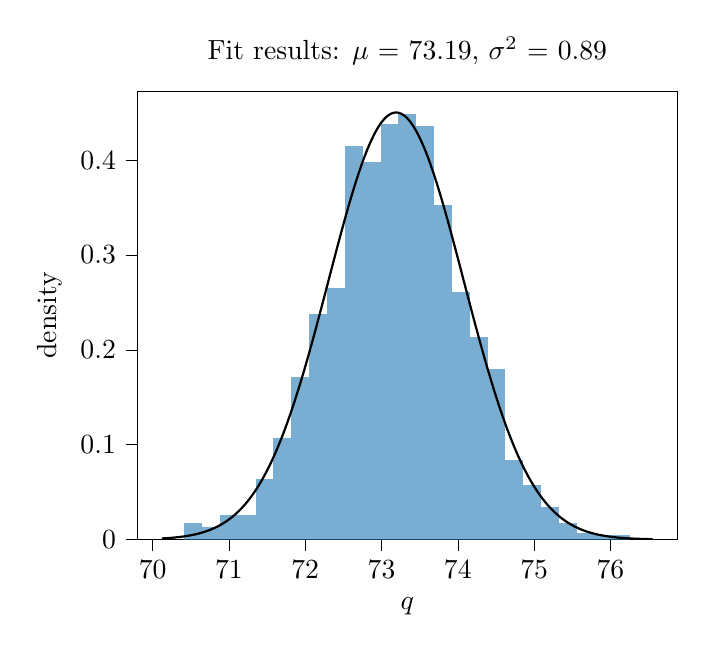
\begin{tikzpicture}

\definecolor{color0}{rgb}{0.12156862745098,0.466666666666667,0.705882352941177}

\begin{axis}[
tick align=outside,
tick pos=left,
title={Fit results: $\mu$ = 73.19,  $\sigma^2$ = 0.89},
xlabel = $q$,
ylabel = density,
x grid style={white!69.0196078431373!black},
xmin=69.8006981611337, xmax=76.8744622631038,
xtick style={color=black},
y grid style={white!69.0196078431373!black},
ymin=0, ymax=0.472848843800874,
ytick style={color=black}
]
\draw[draw=none,fill=color0,fill opacity=0.6] (axis cs:70.4145371947757,0) rectangle (axis cs:70.6483806361631,0.017105461569788);
\draw[draw=none,fill=color0,fill opacity=0.6] (axis cs:70.6483806361632,0) rectangle (axis cs:70.8822240775506,0.0128290961773418);
\draw[draw=none,fill=color0,fill opacity=0.6] (axis cs:70.8822240775506,0) rectangle (axis cs:71.116067518938,0.0256581923546821);
\draw[draw=none,fill=color0,fill opacity=0.6] (axis cs:71.116067518938,0) rectangle (axis cs:71.3499109603255,0.0256581923546836);
\draw[draw=none,fill=color0,fill opacity=0.6] (axis cs:71.3499109603255,0) rectangle (axis cs:71.5837544017129,0.0641454808867052);
\draw[draw=none,fill=color0,fill opacity=0.6] (axis cs:71.5837544017129,0) rectangle (axis cs:71.8175978431004,0.106909134811182);
\draw[draw=none,fill=color0,fill opacity=0.6] (axis cs:71.8175978431003,0) rectangle (axis cs:72.0514412844878,0.17105461569788);
\draw[draw=none,fill=color0,fill opacity=0.6] (axis cs:72.0514412844878,0) rectangle (axis cs:72.2852847258752,0.237338279280824);
\draw[draw=none,fill=color0,fill opacity=0.6] (axis cs:72.2852847258752,0) rectangle (axis cs:72.5191281672627,0.265134654331715);
\draw[draw=none,fill=color0,fill opacity=0.6] (axis cs:72.5191281672627,0) rectangle (axis cs:72.7529716086501,0.414807443067385);
\draw[draw=none,fill=color0,fill opacity=0.6] (axis cs:72.7529716086501,0) rectangle (axis cs:72.9868150500376,0.397701981497572);
\draw[draw=none,fill=color0,fill opacity=0.6] (axis cs:72.9868150500376,0) rectangle (axis cs:73.220658491425,0.438327452725845);
\draw[draw=none,fill=color0,fill opacity=0.6] (axis cs:73.220658491425,0) rectangle (axis cs:73.4545019328124,0.449018366206936);
\draw[draw=none,fill=color0,fill opacity=0.6] (axis cs:73.4545019328125,0) rectangle (axis cs:73.6883453741999,0.436189270029622);
\draw[draw=none,fill=color0,fill opacity=0.6] (axis cs:73.6883453741999,0) rectangle (axis cs:73.9221888155873,0.352800144876878);
\draw[draw=none,fill=color0,fill opacity=0.6] (axis cs:73.9221888155873,0) rectangle (axis cs:74.1560322569748,0.260858288939284);
\draw[draw=none,fill=color0,fill opacity=0.6] (axis cs:74.1560322569748,0) rectangle (axis cs:74.3898756983622,0.213818269622351);
\draw[draw=none,fill=color0,fill opacity=0.6] (axis cs:74.3898756983622,0) rectangle (axis cs:74.6237191397497,0.179607346482785);
\draw[draw=none,fill=color0,fill opacity=0.6] (axis cs:74.6237191397497,0) rectangle (axis cs:74.8575625811371,0.0833891251527167);
\draw[draw=none,fill=color0,fill opacity=0.6] (axis cs:74.8575625811371,0) rectangle (axis cs:75.0914060225245,0.0577309327980382);
\draw[draw=none,fill=color0,fill opacity=0.6] (axis cs:75.0914060225245,0) rectangle (axis cs:75.325249463912,0.0342109231395761);
\draw[draw=none,fill=color0,fill opacity=0.6] (axis cs:75.325249463912,0) rectangle (axis cs:75.5590929052994,0.0171054615697891);
\draw[draw=none,fill=color0,fill opacity=0.6] (axis cs:75.5590929052994,0) rectangle (axis cs:75.7929363466869,0.00641454808867052);
\draw[draw=none,fill=color0,fill opacity=0.6] (axis cs:75.7929363466869,0) rectangle (axis cs:76.0267797880743,0.00427636539244701);
\draw[draw=none,fill=color0,fill opacity=0.6] (axis cs:76.0267797880743,0) rectangle (axis cs:76.2606232294618,0.00427636539244727);
\addplot [thick, black]
table {%
70.1222328930414 0.00111592147405805
70.1286700248113 0.00114433777213781
70.1351071565812 0.00117341571714936
70.1415442883512 0.00120316901217809
70.1479814201211 0.00123361159980918
70.154418551891 0.00126475766521881
70.1608556836609 0.00129662163927844
70.1672928154309 0.00132921820167227
70.1737299472008 0.00136256228402616
70.1801670789707 0.00139666907304857
70.1866042107406 0.00143155401368184
70.1930413425106 0.00146723281226385
70.1994784742805 0.00150372143969809
70.2059156060504 0.00154103613463286
70.2123527378203 0.00157919340664766
70.2187898695903 0.00161821003944673
70.2252270013602 0.00165810309405776
70.2316641331301 0.00169888991203635
70.2381012649 0.0017405881186741
70.24453839667 0.00178321562621047
70.2509755284399 0.0018267906370459
70.2574126602098 0.00187133164695702
70.2638497919797 0.00191685744831217
70.2702869237497 0.00196338713328521
70.2767240555196 0.00201094009706857
70.2831611872895 0.00205953604108271
70.2895983190594 0.00210919497618234
70.2960354508294 0.00215993722585633
70.3024725825993 0.00221178342942252
70.3089097143692 0.00226475454521439
70.3153468461391 0.00231887185375977
70.321783977909 0.00237415696094857
70.328221109679 0.0024306318011905
70.3346582414489 0.00248831864055967
70.3410953732188 0.00254724007992635
70.3475325049887 0.00260741905807226
70.3539696367587 0.00266887885479089
70.3604067685286 0.00273164309396919
70.3668439002985 0.00279573574665098
70.3732810320684 0.00286118113407825
70.3797181638384 0.00292800393071192
70.3861552956083 0.00299622916722804
70.3925924273782 0.00306588223349
70.3990295591481 0.00313698888149247
70.4054666909181 0.00320957522827858
70.411903822688 0.0032836677588274
70.4183409544579 0.00335929332890862
70.4247780862278 0.00343647916790572
70.4312152179978 0.00351525288160358
70.4376523497677 0.00359564245494075
70.4440894815376 0.00367767625472181
70.4505266133075 0.00376138303229168
70.4569637450775 0.00384679192616733
70.4634008768474 0.00393393246462713
70.4698380086173 0.00402283456825312
70.4762751403872 0.00411352855242817
70.4827122721572 0.00420604512978303
70.4891494039271 0.00430041541259379
70.495586535697 0.0043966709151246
70.5020236674669 0.00449484355591772
70.5084607992369 0.00459496566002583
70.5148979310068 0.00469706996118693
70.5213350627767 0.00480118960393648
70.5277721945466 0.00490735814565893
70.5342093263166 0.00501560955857454
70.5406464580865 0.00512597823165743
70.5470835898564 0.00523849897248709
70.5535207216263 0.00535320700902751
70.5599578533963 0.00547013799133476
70.5663949851662 0.00558932799318678
70.5728321169361 0.00571081351363833
70.579269248706 0.00583463147849479
70.585706380476 0.00596081924170579
70.5921435122459 0.00608941458667213
70.5985806440158 0.0062204557274691
70.6050177757857 0.00635398130997969
70.6114549075557 0.0064900304129387
70.6178920393256 0.00662864254888092
70.6243291710955 0.00676985766499678
70.6307663028654 0.00691371614388856
70.6372034346354 0.00706025880422849
70.6436405664053 0.00720952690131126
70.6500776981752 0.00736156212750466
70.6565148299451 0.00751640661259332
70.6629519617151 0.0076741029240098
70.669389093485 0.00783469406695735
70.6758262252549 0.00799822348441635
70.6822633570248 0.00816473505703621
70.6887004887948 0.00833427310290476
70.6951376205647 0.00850688237719966
70.7015747523346 0.00868260807171388
70.7080118841045 0.00886149581425712
70.7144490158745 0.00904359166792475
70.7208861476444 0.00922894213023936
70.7273232794143 0.00941759413215653
70.7337604111842 0.00960959503693704
70.7401975429541 0.00980499263887649
70.7466346747241 0.0100038351618983
70.753071806494 0.010206171258001
70.7595089382639 0.0104120500055622
70.7659460700338 0.0106215209074906
70.7723832018038 0.0108346338892311
70.7788203335737 0.0110514392966154
70.7852574653436 0.0112719878935595
70.7916945971135 0.0114963308595985
70.7981317288835 0.0117245197872666
70.8045688606534 0.0119566066793141
70.8110059924233 0.0121926439457553
70.8174431241932 0.0124326844007548
70.8238802559632 0.0126767812593407
70.8303173877331 0.0129249881339501
70.836754519503 0.0131773590307948
70.8431916512729 0.0134339483460562
70.8496287830429 0.0136948108618995
70.8560659148128 0.013960001742309
70.8625030465827 0.0142295765287366
70.8689401783526 0.0145035911355699
70.8753773101226 0.0147821018454103
70.8818144418925 0.0150651653041659
70.8882515736624 0.0153528385159458
70.8946887054323 0.0156451788377688
70.9011258372023 0.0159422439740718
70.9075629689722 0.0162440919710256
70.9140001007421 0.0165507812106449
70.920437232512 0.0168623704047024
70.926874364282 0.0171789185884409
70.9333114960519 0.017500485114074
70.9397486278218 0.0178271296440871
70.9461857595917 0.0181589121443261
70.9526228913617 0.0184958928768802
70.9590600231316 0.0188381323927463
70.9654971549015 0.0191856915242866
70.9719342866714 0.019538631377468
70.9783714184414 0.019897013323889
70.9848085502113 0.0202608989925818
70.9912456819812 0.0206303502616025
70.9976828137511 0.0210054292493967
71.0041199455211 0.0213861983059479
71.010557077291 0.0217727200036949
71.0169942090609 0.0221650571282338
71.0234313408308 0.0225632726687888
71.0298684726008 0.0229674298084635
71.0363056043707 0.0233775919142549
71.0427427361406 0.0237938225268484
71.0491798679105 0.0242161853501832
71.0556169996805 0.0246447442407807
71.0620541314504 0.0250795631968509
71.0684912632203 0.0255207063471636
71.0749283949902 0.0259682379396923
71.0813655267602 0.0264222223300186
71.0878026585301 0.0268827239695117
71.0942397903 0.0273498073932721
71.1006769220699 0.0278235372078463
71.1071140538399 0.0283039780787001
71.1135511856098 0.0287911947174682
71.1199883173797 0.0292852518689654
71.1264254491496 0.029786214297971
71.1328625809196 0.0302941467757703
71.1392997126895 0.0308091140664743
71.1457368444594 0.0313311809131016
71.1521739762293 0.0318604120234349
71.1586111079992 0.0323968720556363
71.1650482397692 0.0329406256036435
71.1714853715391 0.0334917371823295
71.177922503309 0.0340502712124422
71.1843596350789 0.034616292005303
71.1907967668489 0.0351898637472912
71.1972338986188 0.0357710504841029
71.2036710303887 0.0363599161047748
71.2101081621586 0.0369565243254978
71.2165452939286 0.0375609386732029
71.2229824256985 0.0381732224689345
71.2294195574684 0.0387934388109935
71.2358566892383 0.039421650557878
71.2422938210083 0.0400579203110013
71.2487309527782 0.0407023103972069
71.2551680845481 0.0413548828510601
71.261605216318 0.0420156993969454
71.268042348088 0.0426848214309509
71.2744794798579 0.0433623100025589
71.2809166116278 0.0440482257961217
71.2873537433977 0.0447426291121546
71.2937908751677 0.0454455798484266
71.3002280069376 0.0461571374808678
71.3066651387075 0.0468773610442736
71.3131022704774 0.0476063091128376
71.3195394022474 0.0483440397805027
71.3259765340173 0.0490906106411198
71.3324136657872 0.0498460787684473
71.3388507975571 0.0506105006959699
71.3452879293271 0.0513839323965601
71.351725061097 0.0521664292619596
71.3581621928669 0.0529580460821181
71.3645993246368 0.0537588370243662
71.3710364564068 0.0545688556124486
71.3774735881767 0.0553881547053928
71.3839107199466 0.0562167864762535
71.3903478517165 0.0570548023907089
71.3967849834865 0.0579022531855351
71.4032221152564 0.0587591888469355
71.4096592470263 0.0596256585887644
71.4160963787962 0.0605017108306229
71.4225335105662 0.0613873931758538
71.4289706423361 0.0622827523894102
71.435407774106 0.0631878343756416
71.4418449058759 0.0641026841559732
71.4482820376459 0.0650273458465067
71.4547191694158 0.0659618626355161
71.4611563011857 0.0669062767608843
71.4675934329556 0.0678606294874674
71.4740305647256 0.0688249610843733
71.4804676964955 0.0697993108022025
71.4869048282654 0.0707837168502226
71.4933419600353 0.0717782163735084
71.4997790918053 0.0727828454300205
71.5062162235752 0.0737976389676727
71.5126533553451 0.0748226308013579
71.519090487115 0.07585785358997
71.525527618885 0.0769033388133892
71.5319647506549 0.0779591167494848
71.5384018824248 0.0790252164511059
71.5448390141947 0.080101665723096
71.5512761459646 0.0811884910993002
71.5577132777346 0.08228571781962
71.5641504095045 0.083393369807086
71.5705875412744 0.084511469644985
71.5770246730443 0.0856400385540092
71.5834618048143 0.086779096369484
71.5898989365842 0.0879286615186582
71.5963360683541 0.0890887509980436
71.602773200124 0.0902593803508594
71.609210331894 0.091440563644549
71.6156474636639 0.0926323134484087
71.6220845954338 0.0938346408112951
71.6285217272037 0.095047555239471
71.6349588589737 0.0962710646745578
71.6413959907436 0.0975051754716342
71.6478331225135 0.0987498923774461
71.6542702542834 0.100005218508792
71.6607073860534 0.101271155331048
71.6671445178233 0.102547702636874
71.6735816495932 0.103834858525069
71.6800187813631 0.105132619379632
71.6864559131331 0.106440979849004
71.692893044903 0.107759932825525
71.6993301766729 0.109089469425073
71.7057673084428 0.110429578966946
71.7122044402128 0.111780248953979
71.7186415719827 0.113141465052864
71.7250787037526 0.11451321107475
71.7315158355225 0.115895468956084
71.7379529672925 0.117288218739731
71.7443900990624 0.118691438556335
71.7508272308323 0.120105104606007
71.7572643626022 0.12152919114027
71.7637014943722 0.122963670444341
71.7701386261421 0.124408512819678
71.776575757912 0.125863686566894
71.7830128896819 0.127329157968972
71.7894500214519 0.128804891274838
71.7958871532218 0.130290848683257
71.8023242849917 0.131786990327114
71.8087614167616 0.13329327425804
71.8151985485316 0.13480965643144
71.8216356803015 0.136336090691866
71.8280728120714 0.137872528758822
71.8345099438413 0.139418920212952
71.8409470756113 0.140975212482651
71.8473842073812 0.14254135083108
71.8538213391511 0.144117278343621
71.860258470921 0.145702935915789
71.866695602691 0.147298262241546
71.8731327344609 0.148903193802114
71.8795698662308 0.150517664855229
71.8860069980007 0.152141607424885
71.8924441297707 0.153774951291532
71.8988812615406 0.155417623982793
71.9053183933105 0.157069550764656
71.9117555250804 0.158730654633203
71.9181926568504 0.160400856306804
71.9246297886203 0.162080074218881
71.9310669203902 0.163768224511171
71.9375040521601 0.165465221027556
71.9439411839301 0.167170975308395
71.9503783157 0.16888539658545
71.9568154474699 0.170608391777345
71.9632525792398 0.172339865485623
71.9696897110097 0.17407971999133
71.9761268427797 0.17582785525222
71.9825639745496 0.177584168900546
71.9890011063195 0.179348556241412
71.9954382380894 0.181120910251765
72.0018753698594 0.182901121579969
72.0083125016293 0.18468907854602
72.0147496333992 0.186484667142337
72.0211867651691 0.18828777103522
72.0276238969391 0.190098271566916
72.034061028709 0.191916047758345
72.0404981604789 0.193740976312426
72.0469352922488 0.195572931618092
72.0533724240188 0.197411785754937
72.0598095557887 0.19925740849853
72.0662466875586 0.201109667326368
72.0726838193285 0.202968427424521
72.0791209510985 0.20483355169493
72.0855580828684 0.206704900763395
72.0919952146383 0.208582332988212
72.0984323464082 0.210465704469512
72.1048694781782 0.212354869059299
72.1113066099481 0.214249678372124
72.117743741718 0.216149981796499
72.1241808734879 0.218055626506979
72.1306180052579 0.219966457476956
72.1370551370278 0.221882317492113
72.1434922687977 0.223803047164619
72.1499294005676 0.225728484948
72.1563665323376 0.227658467152728
72.1628036641075 0.229592827962484
72.1692407958774 0.231531399451153
72.1756779276473 0.23347401160051
72.1821150594173 0.235420492318627
72.1885521911872 0.237370667458946
72.1949893229571 0.239324360840097
72.201426454727 0.241281394266399
72.207863586497 0.243241587549083
72.2143007182669 0.245204758528177
72.2207378500368 0.247170723095143
72.2271749818067 0.24913929521617
72.2336121135767 0.251110286956212
72.2400492453466 0.25308350850366
72.2464863771165 0.255058768195758
72.2529235088864 0.257035872544706
72.2593606406564 0.259014626264411
72.2657977724263 0.26099483229797
72.2722349041962 0.262976291845801
72.2786720359661 0.264958804394488
72.2851091677361 0.266942167746248
72.291546299506 0.268926178049112
72.2979834312759 0.27091062982775
72.3044205630458 0.272895316014978
72.3108576948158 0.274880027983876
72.3172948265857 0.276864555580601
72.3237319583556 0.278848687157818
72.3301690901255 0.280832209608794
72.3366062218955 0.282814908402077
72.3430433536654 0.284796567616855
72.3494804854353 0.286776969978892
72.3559176172052 0.288755896897114
72.3623547489752 0.290733128500749
72.3687918807451 0.292708443677103
72.375229012515 0.29468162010993
72.3816661442849 0.296652434318334
72.3881032760548 0.298620661696297
72.3945404078248 0.300586076552732
72.4009775395947 0.302548452152132
72.4074146713646 0.304507560755703
72.4138518031345 0.306463173663092
72.4202889349045 0.308415061254601
72.4267260666744 0.310362993033956
72.4331631984443 0.312306737671527
72.4396003302142 0.314246063048091
72.4460374619842 0.316180736299056
72.4524745937541 0.31811052385918
72.458911725524 0.320035191507707
72.4653488572939 0.321954504414006
72.4717859890639 0.323868227183609
72.4782231208338 0.325776123904716
72.4846602526037 0.327677958195058
72.4910973843736 0.329573493249211
72.4975345161436 0.331462491886297
72.5039716479135 0.333344716598017
72.5104087796834 0.335219929597097
72.5168459114533 0.337087892866058
72.5232830432233 0.338948368206342
72.5297201749932 0.340801117287728
72.5361573067631 0.34264590169809
72.542594438533 0.344482482993432
72.549031570303 0.346310622748224
72.5554687020729 0.348130082605962
72.5619058338428 0.349940624330027
72.5683429656127 0.351742009854751
72.5747800973827 0.353534001336728
72.5812172291526 0.355316361206297
72.5876543609225 0.357088852219247
72.5940914926924 0.358851237508687
72.6005286244624 0.360603280637089
72.6069657562323 0.36234474564844
72.6134028880022 0.36407539712056
72.6198400197721 0.365795000217518
72.6262771515421 0.367503320742152
72.632714283312 0.369200125188646
72.6391514150819 0.370885180795199
72.6455885468518 0.37255825559674
72.6520256786218 0.374219118477643
72.6584628103917 0.375867539224493
72.6648999421616 0.377503288578828
72.6713370739315 0.379126138289886
72.6777742057015 0.380735861167274
72.6842113374714 0.382332231133628
72.6906484692413 0.383915023277175
72.6970856010112 0.385484013904236
72.7035227327812 0.387038980591586
72.7099598645511 0.388579702238728
72.716396996321 0.390105959120014
72.7228341280909 0.391617532936624
72.7292712598609 0.393114206868346
72.7357083916308 0.394595765625195
72.7421455234007 0.396061995498811
72.7485826551706 0.39751268441365
72.7550197869406 0.398947621977902
72.7614569187105 0.400366599534184
72.7678940504804 0.401769410209955
72.7743311822503 0.403155848967613
72.7807683140202 0.404525712654314
72.7872054457902 0.405878800051448
72.7936425775601 0.407214911923792
72.80007970933 0.408533851068272
72.8065168410999 0.409835422362378
72.8129539728699 0.411119432812177
72.8193911046398 0.412385691599926
72.8258282364097 0.413634010131233
72.8322653681796 0.414864202081812
72.8387024999496 0.416076083443754
72.8451396317195 0.417269472571348
72.8515767634894 0.418444190226381
72.8580138952593 0.419600059622962
72.8644510270293 0.420736906471813
72.8708881587992 0.421854559024027
72.8773252905691 0.422952848114262
72.883762422339 0.424031607203381
72.890199554109 0.42509067242052
72.8966366858789 0.426129882604523
72.9030738176488 0.427149079344805
72.9095109494187 0.42814810702156
72.9159480811887 0.429126812845356
72.9223852129586 0.430085046896044
72.9288223447285 0.431022662161022
72.9352594764984 0.431939514572808
72.9416966082684 0.432835463045927
72.9481337400383 0.433710369513067
72.9545708718082 0.434564098960541
72.9610080035781 0.435396519462994
72.9674451353481 0.436207502217377
72.973882267118 0.436996921576152
72.9803193988879 0.437764655079728
72.9867565306578 0.438510583488118
72.9931936624278 0.439234590811808
72.9996307941977 0.439936564341795
73.0060679259676 0.44061639467884
73.0125050577375 0.441273975761873
73.0189421895075 0.441909204895575
73.0253793212774 0.442521982777097
73.0318164530473 0.443112213521934
73.0382535848172 0.443679804688931
73.0446907165872 0.444224667304409
73.0511278483571 0.444746715885409
73.057564980127 0.445245868462043
73.0640021118969 0.445722046598947
73.0704392436669 0.446175175415815
73.0768763754368 0.446605183607033
73.0833135072067 0.44701200346037
73.0897506389766 0.447395570874755
73.0961877707466 0.447755825377109
73.1026249025165 0.448092710138231
73.1090620342864 0.448406171987743
73.1154991660563 0.448696161428075
73.1219362978263 0.448962632647491
73.1283734295962 0.449205543532149
73.1348105613661 0.449424855677198
73.141247693136 0.449620534396893
73.147684824906 0.449792548733741
73.1541219566759 0.449940871466662
73.1605590884458 0.450065479118171
73.1669962202157 0.450166351960567
73.1734333519857 0.450243474021142
73.1798704837556 0.450296833086394
73.1863076155255 0.450326420705252
73.1927447472954 0.450332232191309
73.1991818790653 0.450314266624052
73.2056190108353 0.450272526849114
73.2120561426052 0.450207019477516
73.2184932743751 0.450117754883924
73.224930406145 0.450004747203911
73.231367537915 0.449868014330229
73.2378046696849 0.449707577908079
73.2442418014548 0.449523463329412
73.2506789332247 0.44931569972622
73.2571160649947 0.449084319962862
73.2635531967646 0.448829360627394
73.2699903285345 0.448550862021933
73.2764274603044 0.448248868152031
73.2828645920744 0.447923426715094
73.2893017238443 0.447574589087822
73.2957388556142 0.447202410312693
73.3021759873841 0.446806949083489
73.3086131191541 0.446388267729868
73.315050250924 0.44594643220099
73.3214873826939 0.44548151204821
73.3279245144638 0.444993580406824
73.3343616462338 0.444482713976898
73.3407987780037 0.443948993003175
73.3472359097736 0.443392501254068
73.3536730415435 0.442813325999751
73.3601101733135 0.442211557989342
73.3665473050834 0.441587291427217
73.3729844368533 0.440940623948424
73.3794215686232 0.440271656593243
73.3858587003932 0.439580493780866
73.3922958321631 0.438867243282245
73.398732963933 0.438132016192084
73.4051700957029 0.437374926900003
73.4116072274729 0.436596093060877
73.4180443592428 0.435795635564374
73.4244814910127 0.434973678503685
73.4309186227826 0.43413034914346
73.4373557545526 0.433265777886989
73.4437928863225 0.432380098242589
73.4502300180924 0.431473446789266
73.4566671498623 0.430545963141607
73.4631042816323 0.429597789913978
73.4695414134022 0.428629072683978
73.4759785451721 0.42763995995521
73.482415676942 0.426630603119342
73.488852808712 0.425601156417528
73.4952899404819 0.424551776901129
73.5017270722518 0.423482624391815
73.5081642040217 0.422393861441012
73.5146013357917 0.421285653288757
73.5210384675616 0.420158167821919
73.5274755993315 0.419011575531859
73.5339127311014 0.417846049471482
73.5403498628714 0.416661765211772
73.5467869946413 0.41545890079775
73.5532241264112 0.414237636703904
73.5596612581811 0.412998155789135
73.5660983899511 0.411740643251176
73.572535521721 0.410465286580543
73.5789726534909 0.40917227551401
73.5854097852608 0.407861801987656
73.5918469170308 0.406534060089459
73.5982840488007 0.405189246011482
73.6047211805706 0.403827558001649
73.6111583123405 0.402449196315158
73.6175954441104 0.40105436316551
73.6240325758804 0.399643262675191
73.6304697076503 0.398216100826012
73.6369068394202 0.396773085409165
73.6433439711901 0.395314425974936
73.6497811029601 0.39384033378217
73.65621823473 0.392351021747437
73.6626553664999 0.390846704393994
73.6690924982698 0.389327597800472
73.6755296300398 0.387793919549366
73.6819667618097 0.386245888675338
73.6884038935796 0.384683725613326
73.6948410253495 0.383107652146491
73.7012781571195 0.381517891354015
73.7077152888894 0.37991466755879
73.7141524206593 0.37829820627497
73.7205895524292 0.376668734155444
73.7270266841992 0.375026478939214
73.7334638159691 0.373371669398743
73.739900947739 0.371704535287226
73.7463380795089 0.370025307285858
73.7527752112789 0.368334216951064
73.7592123430488 0.366631496661774
73.7656494748187 0.36491737956669
73.7720866065886 0.363192099531605
73.7785237383586 0.361455891086764
73.7849608701285 0.35970898937433
73.7913980018984 0.357951630095905
73.7978351336683 0.356184049460171
73.8042722654383 0.354406484130641
73.8107093972082 0.352619171173574
73.8171465289781 0.350822348006014
73.823583660748 0.349016252343995
73.830020792518 0.347201122150965
73.8364579242879 0.345377195586371
73.8428950560578 0.343544710954483
73.8493321878277 0.341703906653418
73.8557693195977 0.339855021124457
73.8622064513676 0.337998292801572
73.8686435831375 0.336133960061257
73.8750807149074 0.33426226117262
73.8815178466774 0.332383434247818
73.8879549784473 0.33049771719277
73.8943921102172 0.328605347658219
73.9008292419871 0.326706562991116
73.9072663737571 0.324801600186407
73.913703505527 0.322890695839137
73.9201406372969 0.320974086096975
73.9265777690668 0.319052006613103
73.9330149008368 0.317124692499551
73.9394520326067 0.315192378280928
73.9458891643766 0.313255297848573
73.9523262961465 0.311313684415194
73.9587634279165 0.309367770469925
73.9652005596864 0.307417787733867
73.9716376914563 0.305463967116088
73.9780748232262 0.303506538670159
73.9845119549962 0.301545731551139
73.9909490867661 0.299581773973103
73.997386218536 0.297614893167161
74.0038233503059 0.295645315340057
74.0102604820759 0.293673265633257
74.0166976138458 0.29169896808262
74.0231347456157 0.289722645578597
74.0295718773856 0.287744519827044
74.0360090091555 0.285764811310569
74.0424461409255 0.283783739250483
74.0488832726954 0.281801521569326
74.0553204044653 0.279818374854033
74.0617575362352 0.277834514319666
74.0681946680052 0.275850153773768
74.0746317997751 0.273865505581368
74.081068931545 0.271880780630585
74.0875060633149 0.269896188298878
74.0939431950849 0.267911936419921
74.1003803268548 0.265928231251167
74.1068174586247 0.263945277442017
74.1132545903946 0.261963278002676
74.1196917221646 0.259982434273644
74.1261288539345 0.258002945895919
74.1325659857044 0.256025010781828
74.1390031174743 0.25404882508656
74.1454402492443 0.252074583180348
74.1518773810142 0.250102477621389
74.1583145127841 0.248132699129391
74.164751644554 0.246165436559851
74.171188776324 0.244200876878991
74.1776259080939 0.24223920513943
74.1840630398638 0.24028060445652
74.1905001716337 0.238325255985391
74.1969373034037 0.236373338898687
74.2033744351736 0.234425030365033
74.2098115669435 0.232480505528177
74.2162486987134 0.230539937486829
74.2226858304834 0.228603497275242
74.2291229622533 0.226671353844462
74.2355600940232 0.224743674044299
74.2419972257931 0.222820622605985
74.2484343575631 0.220902362125571
74.254871489333 0.218989053047992
74.2613086211029 0.217080853651851
74.2677457528728 0.215177920034888
74.2741828846428 0.21328040610018
74.2806200164127 0.211388463543008
74.2870571481826 0.209502241838436
74.2934942799525 0.20762188822956
74.2999314117225 0.205747547716493
74.3063685434924 0.203879363046001
74.3128056752623 0.202017474701814
74.3192428070322 0.200162020895676
74.3256799388022 0.19831313755901
74.3321170705721 0.196470958335299
74.338554202342 0.194635614573124
74.3449913341119 0.192807235319859
74.3514284658819 0.190985947316059
74.3578655976518 0.189171874990486
74.3643027294217 0.187365140455772
74.3707398611916 0.18556586350478
74.3771769929616 0.183774161607567
74.3836141247315 0.181990149909001
74.3900512565014 0.180213941227004
74.3964883882713 0.178445646051449
74.4029255200413 0.176685372543645
74.4093626518112 0.174933226536465
74.4157997835811 0.173189311535055
74.422236915351 0.171453728718194
74.4286740471209 0.169726576940204
74.4351111788909 0.16800795273348
74.4415483106608 0.166297950311585
74.4479854424307 0.164596661572948
74.4544225742006 0.162904176105117
74.4608597059706 0.161220581189554
74.4672968377405 0.159545961807042
74.4737339695104 0.157880400643585
74.4801711012803 0.156223978096885
74.4866082330503 0.154576772283322
74.4930453648202 0.152938859045497
74.4994824965901 0.151310311960266
74.50591962836 0.149691202347291
74.51235676013 0.148081599278085
74.5187938918999 0.146481569585575
74.5252310236698 0.144891177874125
74.5316681554397 0.143310486530048
74.5381052872097 0.141739555732573
74.5445424189796 0.140178443465304
74.5509795507495 0.138627205528091
74.5574166825194 0.137085895549375
74.5638538142894 0.135554564998934
74.5702909460593 0.134033263201098
74.5767280778292 0.132522037348342
74.5831652095991 0.131020932515307
74.5896023413691 0.129529991673199
74.596039473139 0.128049255704609
74.6024766049089 0.126578763418689
74.6089137366788 0.125118551566693
74.6153508684488 0.12366865485791
74.6217880002187 0.122229105975923
74.6282251319886 0.120799935595225
74.6346622637585 0.119381172398148
74.6410993955285 0.117972843092161
74.6475365272984 0.116574972427438
74.6539736590683 0.115187583214759
74.6604107908382 0.11381069634369
74.6668479226082 0.112444330801078
74.6732850543781 0.111088503689801
74.679722186148 0.109743230247795
74.6861593179179 0.108408523867337
74.6925964496879 0.107084396114596
74.6990335814578 0.10577085674941
74.7054707132277 0.104467913745289
74.7119078449976 0.103175573309668
74.7183449767676 0.101893839904354
74.7247821085375 0.10062271626618
74.7312192403074 0.0993622034278666
74.7376563720773 0.0981123007390494
74.7440935038473 0.0968730058875184
74.7505306356172 0.0956443149205981
74.7569677673871 0.09442622226669
74.763404899157 0.0932187207569917
74.769842030927 0.0920218016473311
74.7762791626969 0.0908354546401517
74.7827162944668 0.0896596679066084
74.7891534262367 0.0884944281088054
74.7955905580067 0.0873397204221179
74.8020276897766 0.0861955285576294
74.8084648215465 0.0850618347846448
74.8149019533164 0.0839386199533137
74.8213390850864 0.0828258635173031
74.8277762168563 0.0817235435565525
74.8342133486262 0.0806316368000736
74.8406504803961 0.0795501186488258
74.847087612166 0.0784789631986132
74.853524743936 0.0774181432630169
74.8599618757059 0.0763676303963773
74.8663990074758 0.0753273949167726
74.8728361392457 0.074297405929024
74.8792732710157 0.0732776313476934
74.8857104027856 0.072268037920101
74.8921475345555 0.0712685912493114
74.8985846663254 0.0702792558171175
74.9050217980954 0.069299995006987
74.9114589298653 0.0683307711270015
74.9178960616352 0.0673715454327361
74.9243331934051 0.0664222781501093
74.9307703251751 0.0654829284981691
74.937207456945 0.064553454711844
74.9436445887149 0.0636338140646096
74.9500817204848 0.062723962891099
74.9565188522548 0.0618238566096255
74.9629559840247 0.0609334497446431
74.9693931157946 0.0600526959491013
74.9758302475645 0.0591815480267174
74.9822673793345 0.0583199579541389
74.9887045111044 0.0574678769030213
74.9951416428743 0.0566252552619779
75.0015787746442 0.0557920426584157
75.0080159064142 0.0549681879802677
75.0144530381841 0.0541536393975805
75.020890169954 0.0533483443839842
75.0273273017239 0.0525522497380152
75.0337644334939 0.0517653016043174
75.0402015652638 0.0509874454946822
75.0466386970337 0.0502186263089486
75.0530758288036 0.0494587883557414
75.0595129605736 0.0487078753730684
75.0659500923435 0.047965830548739
75.0723872241134 0.0472325965406278
75.0788243558833 0.0465081154967591
75.0852614876533 0.0457923290752343
75.0916986194232 0.0450851784639683
75.0981357511931 0.0443866044002456
75.104572882963 0.0436965471901081
75.111010014733 0.0430149467275384
75.1174471465029 0.0423417425134631
75.1238842782728 0.0416768736745619
75.1303214100427 0.0410202789818738
75.1367585418127 0.0403718968692194
75.1431956735826 0.0397316654514086
75.1496328053525 0.0390995225422449
75.1560699371224 0.0384754056723355
75.1625070688924 0.0378592521066796
75.1689442006623 0.0372509988620538
75.1753813324322 0.0366505827241758
75.1818184642021 0.0360579402646682
75.1882555959721 0.0354730078577905
75.194692727742 0.0348957216969616
75.2011298595119 0.0343260178110538
75.2075669912818 0.0337638320804786
75.2140041230518 0.0332091002530351
75.2204412548217 0.0326617579595431
75.2268783865916 0.0321217407292422
75.2333155183615 0.0315889840049763
75.2397526501314 0.0310634231581391
75.2461897819014 0.0305449935033914
75.2526269136713 0.0300336303131586
75.2590640454412 0.0295292688318867
75.2655011772111 0.0290318442900739
75.2719383089811 0.0285412919180637
75.278375440751 0.0280575469596179
75.2848125725209 0.0275805446852448
75.2912497042908 0.0271102204053026
75.2976868360608 0.0266465094828633
75.3041239678307 0.0261893473463534
75.3105610996006 0.0257386695019525
75.3169982313705 0.0252944115457644
75.3234353631405 0.02485650917575
75.3298724949104 0.0244248982034375
75.3363096266803 0.0239995145653906
75.3427467584502 0.0235802943344517
75.3491838902202 0.0231671737307468
75.3556210219901 0.0227600891324712
75.36205815376 0.0223589770864338
75.3684952855299 0.0219637743183794
75.3749324172999 0.0215744177430765
75.3813695490698 0.0211908444741864
75.3878066808397 0.0208129918338977
75.3942438126096 0.0204407973623356
75.4006809443796 0.0200741988267538
75.4071180761495 0.0197131342304947
75.4135552079194 0.0193575418217324
75.4199923396893 0.0190073601019895
75.4264294714593 0.0186625278344427
75.4328666032292 0.0183229840520012
75.4393037349991 0.0179886680651737
75.445740866769 0.0176595194697152
75.452177998539 0.0173354781540665
75.4586151303089 0.017016484306575
75.4650522620788 0.0167024784225081
75.4714893938487 0.016393401310854
75.4779265256187 0.0160891941009219
75.4843636573886 0.0157897982487293
75.4908007891585 0.0154951555431874
75.4972379209284 0.0152052081120887
75.5036750526984 0.014919898427889
75.5101121844683 0.0146391693132936
75.5165493162382 0.0143629639466479
75.5229864480081 0.0140912258671306
75.5294235797781 0.01382389897976
75.535860711548 0.0135609275602057
75.5422978433179 0.0133022562594118
75.5487349750878 0.0130478301080387
75.5551721068578 0.0127975945207166
75.5616092386277 0.0125514953001199
75.5680463703976 0.0123094786408586
75.5744835021675 0.0120714911331987
75.5809206339375 0.0118374797666017
75.5873577657074 0.0116073919330944
75.5937948974773 0.0113811754304655
75.6002320292472 0.0111587784652991
75.6066691610172 0.010940149655837
75.6131062927871 0.0107252380346809
75.619543424557 0.0105139930513302
75.6259805563269 0.0103063645745658
75.6324176880968 0.0101023028946737
75.6388548198668 0.0099017587255135
75.6452919516367 0.00970468320644086
75.6517290834066 0.0095110279040748
75.6581662151765 0.00932074481392163
75.6646033469465 0.00913378636185164
75.6710404787164 0.008950105405438
75.6774776104863 0.00876965523515187
75.6839147422562 0.00859238957542289
75.6903518740262 0.00841826258556249
75.6967890057961 0.00824722886055885
75.703226137566 0.00807924343173801
75.7096632693359 0.00791426176729988
75.7161004011059 0.00775223977272702
75.7225375328758 0.00759313379107435
75.7289746646457 0.00743690060313509
75.7354117964156 0.00728349742749108
75.7418489281856 0.00713288192044556
75.7482860599555 0.00698501217584637
75.7547231917254 0.00683984672479516
75.7611603234953 0.00669734453525042
75.7675974552653 0.0065574650115226
75.7740345870352 0.00642016799366898
75.7804717188051 0.00628541375678449
75.786908850575 0.0061531630101938
75.793345982345 0.00602337689654948
75.7997831141149 0.00589601699083315
75.8062202458848 0.0057710452992663
75.8126573776547 0.00564842425812998
75.8190945094247 0.00552811673249979
75.8255316411946 0.00541008601489301
75.8319687729645 0.00529429582383449
75.8384059047344 0.00518071030234039
75.8448430365044 0.00506929401632589
75.8512801682743 0.00496001195293416
75.8577173000442 0.00485282951879267
75.8641544318141 0.00474771253819606
75.8705915635841 0.00464462725122156
75.877028695354 0.00454354031177421
75.8834658271239 0.00444441878556789
75.8899029588938 0.00434723014804128
75.8963400906638 0.00425194228221453
75.9027772224337 0.00415852347648408
75.9092143542036 0.00406694242236124
75.9156514859735 0.00397716821215393
75.9220886177435 0.00388917033659678
75.9285257495134 0.00380291868242762
75.9349628812833 0.00371838352991428
75.9414000130532 0.00363553555033502
75.9478371448232 0.00355434580341107
75.9542742765931 0.00347478573469592
75.960711408363 0.00339682717292112
75.9671485401329 0.00332044232730313
75.9735856719029 0.00324560378480951
75.9800228036728 0.00317228450738888
75.9864599354427 0.00310045782916441
75.9928970672126 0.00303009745359514
75.9993341989826 0.00296117745060351
76.0057713307525 0.00289367225367321
76.0122084625224 0.00282755665691731
76.0186455942923 0.00276280581212044
76.0250827260622 0.00269939522575382
76.0315198578322 0.00263730075596601
76.0379569896021 0.00257649860955223
76.044394121372 0.00251696533890081
76.0508312531419 0.0024586778389207
76.0572683849119 0.00240161334394973
76.0637055166818 0.00234574942464705
76.0701426484517 0.00229106398486862
76.0765797802216 0.00223753525852914
76.0830169119916 0.00218514180645019
76.0894540437615 0.00213386251319783
76.0958911755314 0.00208367658390852
76.1023283073013 0.00203456354110654
76.1087654390713 0.00198650322151267
76.1152025708412 0.00193947577284718
76.1216397026111 0.001893461650626
76.128076834381 0.00184844161495304
76.134513966151 0.00180439672730845
76.1409510979209 0.00176130834733554
76.1473882296908 0.00171915812962541
76.1538253614607 0.001677928020502
76.1602624932307 0.00163760025480723
76.1666996250006 0.00159815735268893
76.1731367567705 0.00155958211639058
76.1795738885404 0.00152185762704478
76.1860110203104 0.00148496724147208
76.1924481520803 0.00144889458898432
76.1988852838502 0.00141362356819497
76.2053224156201 0.001379138343836
76.2117595473901 0.00134542334358369
76.21819667916 0.00131246325489232
76.2246338109299 0.00128024302183803
76.2310709426998 0.00124874784197243
76.2375080744698 0.00121796316318814
76.2439452062397 0.00118787468059524
76.2503823380096 0.0011584683334107
76.2568194697795 0.00112973030186051
76.2632566015495 0.00110164700409618
76.2696937333194 0.00107420509312509
76.2761308650893 0.00104739145375606
76.2825679968592 0.00102119319956032
76.2890051286292 0.000995597669849079
76.2954422603991 0.000970592426667228
76.301879392169 0.00094616525180461
76.3083165239389 0.000922304143824658
76.3147536557089 0.000898997315111775
76.3211907874788 0.000876233188936876
76.3276279192487 0.000854000396542061
76.3340650510186 0.000832287774245277
76.3405021827886 0.00081108436056442
76.3469393145585 0.000790379393362068
76.3533764463284 0.000770162307010669
76.3598135780983 0.000750422729579246
76.3662507098683 0.000731150480041066
76.3726878416382 0.000712335565503328
76.3791249734081 0.000693968178458637
76.385562105178 0.000676038694059251
76.391999236948 0.000658537667413523
76.3984363687179 0.000641455830905478
76.4048735004878 0.000624784091537294
76.4113106322577 0.000608513528295518
76.4177477640276 0.000592635389540516
76.4241848957976 0.000577141090419735
76.4306220275675 0.000562022210305232
76.4370591593374 0.00054727049025502
76.4434962911073 0.000532877830498911
76.4499334228773 0.00051883628794865
76.4563705546472 0.000505138073732943
76.4628076864171 0.000491775550756892
76.469244818187 0.000478741231286455
76.475681949957 0.00046602777455766
76.4821190817269 0.00045362798441112
76.4885562134968 0.000441534806951361
76.4949933452667 0.00042974132823148
76.5014304770367 0.000418240771962853
76.5078676088066 0.000407026497250371
76.5143047405765 0.000396091996352696
76.5207418723464 0.000385430892467998
76.5271790041164 0.00037503693754486
76.5336161358863 0.000364904010118771
76.5400532676562 0.000355026113173684
76.5464903994261 0.000345397372029049
76.5529275311961 0.000336012032251984
};
\end{axis}

\end{tikzpicture}

\end{center}
\end{subfigure}
\caption{2000 alpha complexes on 300 points drawn from a uniform distribution.}
\label{fig:300fit}
\end{figure}

What we can take from the plot and the generated data is that we have an average $q$-value of $73.19\%$ and values ranging from  $70\%$ to $76\%$. Meaning that more than two thirds of simplices are part of an apparent pair in all filtrations we constructed, while on average almost three quarters are part of an apparent pair.

The following figure shows a plot where we map the size of the two dimensional point clouds to the average mean $q$-values. We observe an almost monotone downtrend, which indicates that the percentage of simplices in apparent pairs decreases with increasing length of the filtrations. In the following two figures the scattered points are the actually calculated values and the line segments between them are linearly interpolated.

\begin{figure}[H]
%\centering%
\begin{subfigure}[c]{0.95\textwidth}
\begin{center}
% This file was created by tikzplotlib v0.9.2.
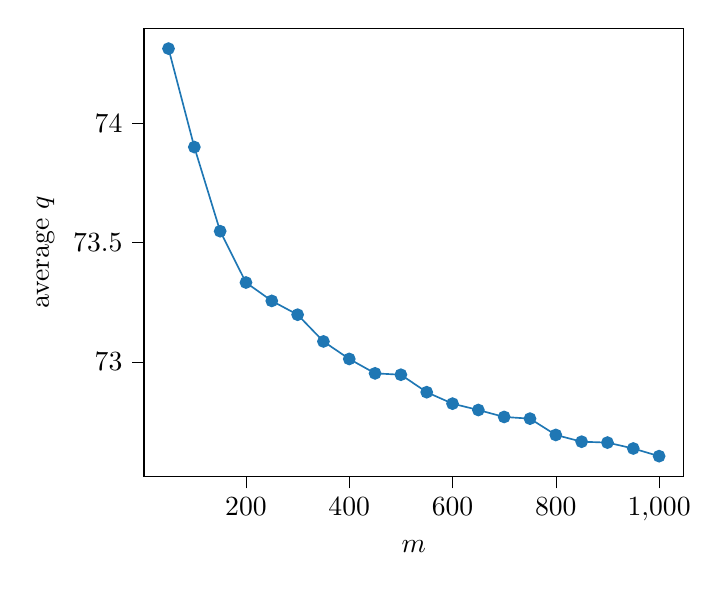
\begin{tikzpicture}

\definecolor{color0}{rgb}{0.12156862745098,0.466666666666667,0.705882352941177}
\definecolor{color1}{rgb}{0.976470588235294,0.450980392156863,0.0235294117647059}

\begin{axis}[
tick align=outside,
tick pos=left,
xlabel = $m$,
ylabel = average $q$,
x grid style={white!69.0196078431373!black},
xmin=2.5, xmax=1047.5,
xtick style={color=black},
y grid style={white!69.0196078431373!black},
%´ymin=72, ymax=91,
ymin=72.5198618350407, ymax=74.3989386078973,
ytick style={color=black},
scatter/classes={a={mark=o,draw=black}}
]
\addplot[scatter, scatter src=explicit symbolic, semithick, color0]
table {%
50 74.3135260273129
100 73.9007987162947
150 73.548228008839
200 73.3330687122862
250 73.256039993344
300 73.1981969846523
350 73.0861031936403
400 73.0127258791942
450 72.9523915686429
500 72.9466183308799
550 72.873379839116
600 72.8254219384188
650 72.7987235551989
700 72.7696569674668
750 72.7625372033231
800 72.6942015413158
850 72.6658903806182
900 72.6621935833012
950 72.6374432276665
1000 72.6052744156251
};

\end{axis}

\end{tikzpicture}

\end{center}
\end{subfigure}
\caption{Means of 2000 averaged alpha complexes on differently sized points clouds drawn from a uniform distribution.}
\label{fig:2d_means}
\end{figure}

Since the $q$-values are well fitted by normal distributions, we generated a similar plot for the standard deviations.

\begin{figure}[H]
%\centering%
\begin{subfigure}[c]{0.95\textwidth}
\begin{center}
% This file was created by tikzplotlib v0.9.2.
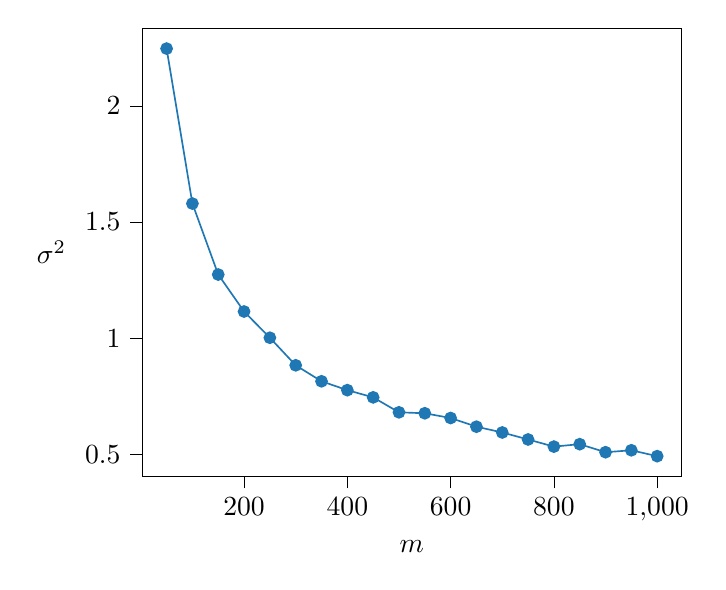
\begin{tikzpicture}

\definecolor{color0}{rgb}{0.12156862745098,0.466666666666667,0.705882352941177}
\definecolor{color1}{rgb}{0.976470588235294,0.450980392156863,0.0235294117647059}

\begin{axis}[
tick align=outside,
tick pos=left,
ylabel = $\sigma^2$,
xlabel = $m$,
ylabel style={rotate=-90},
x grid style={white!69.0196078431373!black},
xmin=2.5, xmax=1047.5,
xtick style={color=black},
y grid style={white!69.0196078431373!black},
ymin=0.404619119795701, ymax=2.33384993531293,
ytick style={color=black},
scatter/classes={a={mark=o,draw=black}}
]
\addplot[scatter, scatter src=explicit symbolic, semithick, color0]
table {%
50 2.24615762551669
100 1.5792435037505
150 1.27389257927507
200 1.1147961093539
250 1.00194489752104
300 0.883268619119549
350 0.814502452409831
400 0.776380080599139
450 0.745367391163501
500 0.681014417056458
550 0.676891814240733
600 0.656527982762773
650 0.619120834767529
700 0.59424703343731
750 0.564172814777307
800 0.533426280089837
850 0.543871439397632
900 0.509264003967767
950 0.517621741132293
1000 0.492311429591938
};
\end{axis}

\end{tikzpicture}

\end{center}
\end{subfigure}
\caption{Standard deviations of 2000 averaged alpha complexes on differently sized points clouds drawn from a uniform distribution.}
\label{fig:2d_stds}
\end{figure}

As we can see, the larger the complex, the less variance we have with respect to the $q$-values. This could be explained by some local configurations containing lots of apparent pairs while others are containing only a few. The larger the complex, the more likely that we have these evenly distributed, while in a smaller complex the probability for extreme cases is higher. 

Overall this means the larger the complex the fewer of its elements are part of an apparent pair percentage wise, however larger complexes are more similar to one another in that regard than smaller complexes.

We have also calculated an average $q$-value for two-dimensional alpha complexes on 5000 points and got a mean of $72.20$ and a standard deviation of $0.20$. It would be interesting to explore if and to what value these values converge. Or if they are bounded somehow in a random setting. 

As we have previously seen, it is theoretically possible to have a filtration of any length with a single apparent pair between edges and triangles. 

One might expect a similar looking curve when increasing the dimension of the points instead of their number, since an alpha complex constructed on $100$ points in dimension two is expected to be much smaller than one in dimension three. The mean value of the $q$-values however increases substantially.

\begin{figure}[H]
%\centering%
\begin{subfigure}[c]{0.95\textwidth}
\begin{center}
% This file was created by tikzplotlib v0.9.2.
\begin{tikzpicture}

\definecolor{color0}{rgb}{0.12156862745098,0.466666666666667,0.705882352941177}

\begin{axis}[
tick align=outside,
tick pos=left,
xlabel = dimension,
ylabel = average $q$,
ylabel style={rotate=-90},
x grid style={white!69.0196078431373!black},
xmin=1.8, xmax=6.2,
xtick style={color=black},
y grid style={white!69.0196078431373!black},
ymin=72.9311706171997, ymax=100.719766845615,
ytick style={color=black},
scatter/classes={%
    a={mark=o,draw=color0}}
]
\addplot [scatter,only marks,%
    scatter src=explicit symbolic,color0]
table {%
2 74.1942886275822
3 90.1118873880867
4 95.401135865881
5 98.4740519194136
6 99.4566488352329
};
\end{axis}

\end{tikzpicture}

\end{center}
\end{subfigure}
\caption{Means of alpha complexes on 30 points in varying dimensions, averaged over 50 runs.}
\label{fig:means_by-dimension}
\end{figure}

While in dimension two, on average, about three quarters of all simplices are part of an apparent pair on an alpha complex on thirty points, in dimension six we have an average $q$-value of $99.46 \%$. A partial explanation is that with increasing dimension more simplices can be paired with lower or higher dimensional simplices and the number of maximal faces of the complex decreases. 

Note that in the last experiment we averaged the values over $50$ runs instead of $2000$. This is partially caused by the fact that simplicial complexes grow quite fast in higher dimensions and that running time was a limiting factor when performing the experiments. In the remainder of this chapter we will see values averaged over different amounts of tries due to this.

We carried out the same experiments for point clouds sampled from a multivariate Gaussian and a Gaussian mixture model. For the multivariate Gaussian we have taken the point $(0,0)$ as mean and the identity matrix as covariance matrix. For the mixture model we chose $(0,0)$, $(1,1)$ and $(0,3)$ as mean values and each covariance matrix was again the identity matrix. The values for the Gaussian mixture were picked to get some overlap between the areas of high density but not too much, since if they are too close we expect a similar set of points to that of a single multivariate distribution and if they are too far away they locally would also have the same structure as a point cloud drawn from a single multivariate distribution. 

We observe the same general behavior for all three distributions. However there are noteable differences in the values of the means. Figure \ref{fig:2d_all_compared} shows the development of the means for all three generated data sets in one diagram. The continuous line represents the uniform distribution, the dotted line corresponds to the multivariate Gaussian and the dashed line corresponds to the Gaussian mixture model.

\begin{figure}[H]
%\centering%

\begin{subfigure}[c]{0.99\textwidth}
\begin{center}
% This file was created by tikzplotlib v0.9.2.
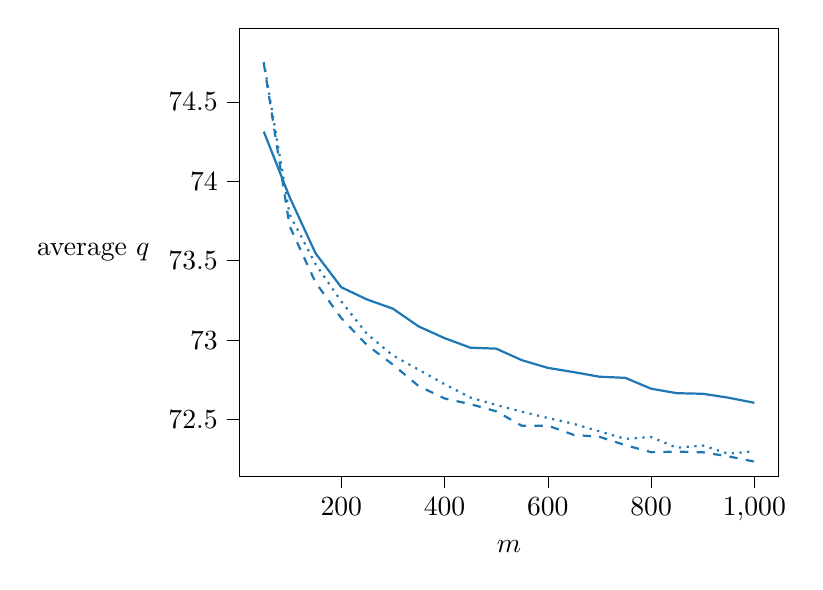
\begin{tikzpicture}

\definecolor{color0}{rgb}{0.12156862745098,0.466666666666667,0.705882352941177}

\begin{axis}[
tick align=outside,
tick pos=left,
xlabel = $m$,
ylabel = average $q$,
ylabel style={rotate=-90},
x grid style={white!69.0196078431373!black},
xmin=2.5, xmax=1047.5,
xtick style={color=black},
y grid style={white!69.0196078431373!black},
ymin=72.1408722544235, ymax=74.9646784830289,
ytick style={color=black}
]
\addplot [thick, color0, dotted]
table {%
50 74.751221902748
100 73.7920620385357
150 73.4803739655178
200 73.244056612421
250 73.0385644533163
300 72.9036301595062
350 72.8136863565804
400 72.7229801131946
450 72.638716960172
500 72.5917237632603
550 72.5491378420652
600 72.5096471359426
650 72.4730934536537
700 72.4249485291089
750 72.378279089354
800 72.3896536253948
850 72.3218743554731
900 72.3368743405545
950 72.2845377486291
1000 72.3004042654642
};

\addplot [thick, color0, dashed]
table {%
50 74.7440091823553
100 73.7186939751261
150 73.3647881875886
200 73.1389162360907
250 72.9682849309851
300 72.8459369302215
350 72.7103796794705
400 72.6327957832213
450 72.5969537461766
500 72.5518642799392
550 72.4602006772107
600 72.461873858482
650 72.4035463050674
700 72.3909778284513
750 72.3387470840265
800 72.294478801029
850 72.2975470698247
900 72.2937838331733
950 72.2676937029656
1000 72.2349609142709
};
\addplot[thick, color0]
table {%
50 74.3135260273129
100 73.9007987162947
150 73.548228008839
200 73.3330687122862
250 73.256039993344
300 73.1981969846523
350 73.0861031936403
400 73.0127258791942
450 72.9523915686429
500 72.9466183308799
550 72.873379839116
600 72.8254219384188
650 72.7987235551989
700 72.7696569674668
750 72.7625372033231
800 72.6942015413158
850 72.6658903806182
900 72.6621935833012
950 72.6374432276665
1000 72.6052744156251
};
\end{axis}

\end{tikzpicture}


\end{center}
\end{subfigure}


%\begin{subfigure}[c]{0.99\textwidth}
%\begin{center}
%% This file was created by tikzplotlib v0.9.2.
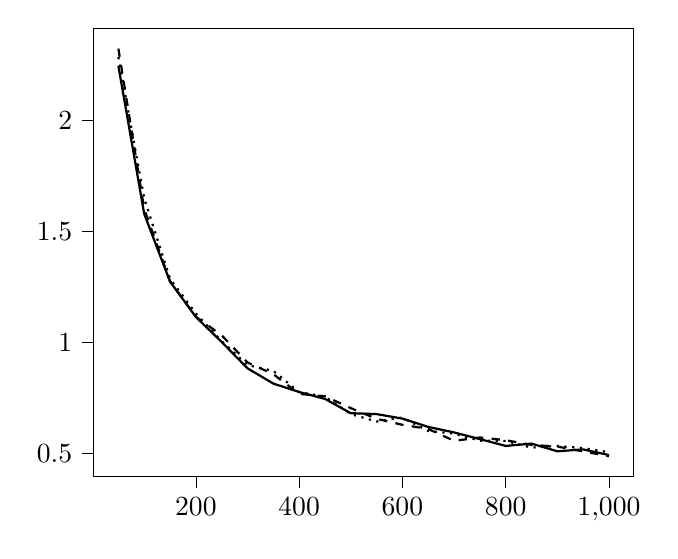
\begin{tikzpicture}

\definecolor{color0}{rgb}{0.12156862745098,0.466666666666667,0.705882352941177}

\begin{axis}[
tick align=outside,
tick pos=left,
x grid style={white!69.0196078431373!black},
xmin=2.5, xmax=1047.5,
xtick style={color=black},
y grid style={white!69.0196078431373!black},
ymin=0.395394258663213, ymax=2.41598322003903,
ytick style={color=black}
]
\addplot [thick, black, dashed]
table {%
50 2.32413826724922
100 1.6017798725875
150 1.27569876899754
200 1.11569841878204
250 1.03198710689561
300 0.909575719051176
350 0.85673532804327
400 0.768062421883222
450 0.757084132537467
500 0.703841068123042
550 0.655567344924125
600 0.628660144146404
650 0.609964523254271
700 0.55626807435996
750 0.571403742096503
800 0.559237227591519
850 0.537978856444726
900 0.530597459789274
950 0.508673050702853
1000 0.487239211453023
};

\addplot [thick, black]
table {%
50 2.24615762551669
100 1.5792435037505
150 1.27389257927507
200 1.1147961093539
250 1.00194489752104
300 0.883268619119549
350 0.814502452409831
400 0.776380080599139
450 0.745367391163501
500 0.681014417056458
550 0.676891814240733
600 0.656527982762773
650 0.619120834767529
700 0.59424703343731
750 0.564172814777307
800 0.533426280089837
850 0.543871439397632
900 0.509264003967767
950 0.517621741132293
1000 0.492311429591938
};

\addplot [thick, black, dotted]
table {%
50 2.2861808651118
100 1.64986784602092
150 1.28683882516498
200 1.13016921748758
250 1.00585682814682
300 0.897678965646122
350 0.871678397927158
400 0.776296030264333
450 0.755134146237627
500 0.67702370736897
550 0.64349690377966
600 0.661206342404475
650 0.601008063114883
700 0.588765385643078
750 0.556921114871381
800 0.555686528665616
850 0.525900473767235
900 0.533350195248551
950 0.523497215225528
1000 0.505036296302693
};

\end{axis}

\end{tikzpicture}

%\subcaption{Standard deviation of $q$-values compared between differently drawn point clouds.}
%\end{center}
%\end{subfigure}

\caption{Mean $q$-values compared between differently drawn point clouds.}
\label{fig:2d_all_compared}
\end{figure}

Let us consider the difference we see between the means of the two samples from Gaussian distributions and the uniform distribution. Note that the difference in number of simplices is quite small for all cases we considered. For example the average number of elements in filtrations on $1000$ points is $5957.4$ in case of the uniform distribution and $5971.16$ in case of the Gaussian mixture. Therefore the gap between the curves is not explicable by a difference in number of elements of the filtrations. 

A possible explanation for the differing developments of means is that point sets with one or several clusters and some outliers yield bad local structures with respect to simplices being a part of an apparent pair. Although the difference between the single multivariate Gaussian and the Gaussian mixture model is quite small it is nevertheless consistent for different sizes of point clouds. What exactly this potentially \enquote{bad} structure is remains to be uncovered.

The similar curves in standard deviation strengthen the intuition, that these mainly depend on the size of the complex and that \enquote{good} and \enquote{bad} local configurations appear more evenly distributed. 

%One practical observation that has been made by several authors and people concerned with persistent homology is that although the running time in theory is cubic we only see slightly super linear running times in practice. Perhaps the canonical persistence pairs defined by the apparent pairs might be useful to explore this phenomenon. In the next section we will look at apparent pairs and the running time of the standard reduction scheme.

\section{Apparent Pairs in Standard Reduction}

A natural question is if there is some kind of connection between the value $q$ for some filtration $F$ of simplicial complex $K$ and the number of additions $\operatorname{add}(B)$ needed to reduce the boundary matrix $B$ of $F$. We can guess from what we discussed in Chapter \ref{ch:connection} that only considering the number of apparent pairs does not suffice to explain the number of additions. Nevertheless we checked if there is some linear correlation between the value of $q$ and $\frac{\operatorname{add}(B)}{m}$, where $m$ is the number of elements in $K$. We calculated the correlation coefficient via \textbf{numpy.corrcoef} of the Python library \textbf{numpy}. The following figure shows a scatter plot of $100$ alpha complexes on $100$ points. On the $x$-axis we have the values of $q$ and on the $y$-axis we have $\frac{\operatorname{add}(B)}{m}$. Above the plot we display the calculated linear correlation coefficient.

\begin{figure}[H]
%\centering%
\begin{subfigure}[c]{0.95\textwidth}
\begin{center}
% This file was created by tikzplotlib v0.9.2.
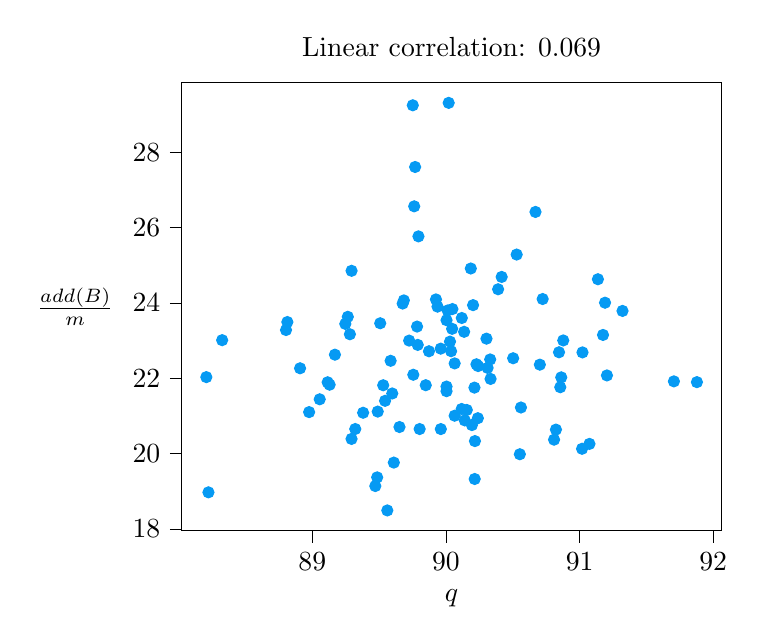
\begin{tikzpicture}

\definecolor{color0}{rgb}{0.0235294117647059,0.603921568627451,0.952941176470588}

\begin{axis}[
tick align=outside,
tick pos=left,
title={Linear correlation: 0.069},
ylabel style={rotate=-90},
xlabel = $q$,
ylabel = $\frac{\operatorname{add}(B)}{m}$,
x grid style={white!69.0196078431373!black},
xmin=88.0233754034327, xmax=92.0615058308513,
xtick style={color=black},
y grid style={white!69.0196078431373!black},
ymin=17.9477669720933, ymax=29.8578650389586,
ytick style={color=black}
]
\addplot [only marks, mark=*, draw=color0, fill=color0, colormap/viridis]
table{%
x                      y
90.2169101372289 20.3315626383355
91.0737386804657 20.257007330746
90.5027932960894 22.532015470563
89.5980107749689 21.596353087443
89.2811020232458 23.1696082651743
90.5611135276207 21.2235754675946
90.3902643726395 24.3646663869073
91.0184787279759 20.1267726686721
91.1903738719381 24.0077352814783
88.9760348583878 21.1015250544662
89.8488120950324 21.8159827213823
90.1175446234218 21.1841532433609
90.0384779820436 22.7195382642155
90.1859057501081 24.9165585819282
88.8132709485325 23.4942577626542
90.1359053046909 23.2341078474353
90.0650759219089 22.3952277657267
90.0128589798543 23.8011144449207
90.5528950805398 19.9821506312582
91.8779544477868 21.8972926514826
90.2281532501076 22.3723633232889
90.1559020044543 21.1576837416481
91.7056571671629 21.9179072735006
90.1185770750988 23.6012296881862
88.3253170091823 23.0126803672934
90.3032891926527 23.052541648868
90.7234798047048 24.1056369285397
91.3210773834972 23.7892261650278
89.7624190064795 26.5680345572354
89.6849374190764 24.0690548122572
89.5611418832552 18.4891350660418
89.3801473775466 21.0840918942349
90.8627284317892 22.0246493837654
90.5291240551356 25.2867941307248
90.0482244629548 23.8386672512056
90.0042176296921 21.7794179671025
91.2046686119216 22.0754481033764
90.4168457241083 24.6923076923077
89.7838066977533 23.3738872403561
89.3212278426286 20.6519671422395
90.8459869848156 22.6911062906725
90.8229211546747 20.6363636363636
89.7941305300044 25.7700394218134
90.8554572271386 21.7623261694058
90.3115663679044 22.2765685019206
90.2028485110056 23.9430297798878
89.1294932871373 21.8289302728454
89.7888841016803 22.8866867729427
90.0302114803625 22.9741044454035
90.2386117136659 20.939262472885
89.5859473023839 22.4642409033877
90.2131361461505 21.7516311439756
89.9368421052632 23.9031578947368
90.0650759219089 21.0056399132321
89.7245299519021 23.0008745080892
90.0043271311121 23.5430549545651
89.4894894894895 21.1149721149721
89.471346068414 19.1372723234118
89.1692040017399 22.6267942583732
89.2468437091859 23.4453635176317
90.6699547883272 26.4188244965064
89.9608865710561 22.787049109083
89.5444685466377 21.4008676789588
88.8030888030888 23.2818532818533
89.8728627794827 22.7176676896098
90.8776480760917 23.0051880674449
89.9615548910722 20.6505766766339
89.5303748384317 21.8147350280052
88.2069267864971 22.0306882946076
89.7692642577275 27.6129734436221
89.6760259179266 23.985313174946
89.7516930022573 29.2523702031603
89.2934547030776 20.3892501083658
89.1147818720881 21.8936891147819
89.2936472678809 24.8551754775655
90.3308981521272 22.50021486893
89.8030634573304 20.6516411378556
88.2226980728051 18.9700214132762
90.0461990760185 23.3137337253255
90.3337667967057 21.9826614651062
89.6522112494633 20.7050236152855
89.6098202542744 19.7601928978518
89.755679382769 22.0938705529361
90.00429000429 21.6572286572287
90.1943844492441 20.7568034557235
88.9083735203858 22.2656729504603
90.2407002188184 22.3242888402626
91.0216718266254 22.687748783724
89.925208974923 24.0950285965684
91.1370514483355 24.63121487246
89.0553474823138 21.4419475655431
89.2655367231638 23.6327683615819
89.5080539834567 23.4614714845451
90.8089792460822 20.3689114781872
90.2150065818341 19.3242650285213
90.7025662599916 22.3618005889777
90.020366598778 29.3164969450102
89.4852617685878 19.3677958644963
90.1408450704225 20.8813486982501
91.1752044769694 23.1510977184675
};
\end{axis}

\end{tikzpicture}

\end{center}
\end{subfigure}
\caption{Value of $q$ related to the number of additions per column in the standard reduction scheme for some filtration $F$ with $m$ elements.}
\label{fig:correlation_3d}
\end{figure}

Unfortunately but not unsurprisingly there is no or only a very small linear correlation between the number of additions divided by the number of elements in the complex and $q$. This means that the complicatedness of persistent homology computations is not explicable by the number of critical cells of the apparent gradient. \\ 

In the following we will try to illustrate how much of the work during reduction is done on apparent pairs. To be more precise, this means how much work is done on the tails of apparent pairs since the columns corresponding to the heads of the apparent pairs are reduced from the beginning. See the proof of Lemma \ref{lem:app_is_pers}. Note that we are not counting the number of column additions as in Definition \ref{def:col_red_steps} but the total number of addition operations, i.e. the number of additions of non-zero elements during the addition of columns.

As a preprocessing step for reduction we can set all tails of apparent pairs to zero. This will save us all additions needed to reduce the respective columns. It comes at the cost of finding the apparent pairs first however. Furthermore there are other more potent preprocessing steps that can be done. 

For example for each simplex $\sigma$ of a filtration one can just set the column of the youngest facet to zero, since it creates a cycle with the other facets of the simplex that has to be closed by simplex $\sigma$ at the latest. This procedure also implicitly sets the columns corresponding to tails of apparent pairs to zero.

In Section \ref{sec:twist} we already discussed the so called twisted reduction scheme which starts in the highest dimension and works its way down. Preprocessing with apparent pairs yields no improvement for this procedure, as every column corresponding to the tail of an apparent pair will just be set to zero without doing any calculations when its head is processed. Nevertheless the analysis we do in this section still tells us how much of the improvements of the twisted reduction scheme over the standard reduction scheme stem from columns corresponding to tails of apparent pairs. Recall that we refer to the process of setting columns to zero when we know that they correspond to a simplex creating a homology class as \textbf{clearing}. See Section \ref{sec:twist}.

We have already seen that in the setting of alpha complexes on random point clouds of a fixed size that the percentage of simplices that are part of an apparent pair increases with dimension. This means that we would expect higher speedups for the standard reduction scheme, see Algorithm \ref{algo:column_reduction_algorithm}, in higher dimensions. We will try to measure the speedups in the following way. 

For given filtration $F$, let $SRT$ (\textbf{standard reduction time}) denote the time it takes to construct and reduce some boundary matrix via the standard reduction scheme. Let $ART$ (\textbf{apparent reduction time}) denote the time it takes to find all apparent pairs, clear columns in the boundary matrix corresponding to tails of apparent pairs, and do the standard reduction. We will consider \[
s \coloneqq \frac{SRT}{ART},
\] i.e., the factor by which the overall reduction time decreases when we do clearing in the preprocessing via apparent pairs. If $s > 1$, we save time, if $s<1$ we loose time, i.e., the cost for finding the apparent pairs and clearing the columns is higher than the gain compared to the standard reduction. 

The implementations of the algorithms can be found on \href{https://github.com/IvanSpirandelli/Masterarbeit/blob/master/Algorithms/column_algo/column_algorithm.py}{[GitHub]}, see \cite{github}.

We will average each setup of parameters over hundreds of runs to make sure the values we are seeing are no anomaly caused by some external factor.

All experiments were done on an \enquote{Intel Core i7-3770 CPU \@ 3.40GHz~x~8} processor. 

Note that the implemented algorithms are not optimized for speed since the primary interest was not to develop a fast persistent homology computation but to analyse and compare examples with respect to additions in the boundary matrices. 

Hence, the consideration of how many additions we save by clearing the apparent columns is more meaningful. For a given filtration $F$, let $SRA$ (\textbf{standard reduction additions}), denote the number of additions in the standard reduction process and let $ARA$ (\textbf{apparent reduction additions}) denote the number of additions on the boundary matrix which was cleared by setting tails of apparent pairs to zero. Then we define
\[
a \coloneqq 100 (1- \frac{ARA}{SRA}),
\]
i.e., the percentage of additions that are not necessary when reducing the cleared boundary matrix. Or in other words: A high $a$-value implies that the clearing yields a big improvement while a low value implies that even after clearing we still have lots of additions to do. The following table shows the average $s$ and $a$ values for alpha complexes on $30$ points in dimensions two and three drawn from the previously mentioned distributions. We averaged the values over $200$ runs.



 \begin{table}[H]
     \begin{center}
     \begin{tabular}{|c|c|c|c|}
     \hline
     & \multicolumn{3}{|c|}{Execution Time Speedup} \\ \cline{1-4}
     Sample distribution & Uniform & Multivariate Normal & Gaussian 		Mixture\\ \hline
     dimension two & 1.96 & 2.09 & 2.13\\ \hline
     dimension three & 3.02 & 3.37 & 3.67\\ \hline

     \end{tabular}
     
     \caption{$s$-value for alpha complexes on randomly generated point clouds.}
     \label{tab:time_STA_TWI}
     \end{center}
 \end{table}




 \begin{table}[H]
     \begin{center}
     \begin{tabular}{|c|c|c|c|}
     \hline
     & \multicolumn{3}{|c|}{Percentage of Saved Additions} \\ \cline{1-4}
     Sample distribution & Uniform & Multivariate Normal & Gaussian 		Mixture\\ \hline
     dimension two & 66.64 & 69.90 & 70.98 \\ \hline
     dimension three & 68.98 & 73.64 & 76.75 \\ \hline

     \end{tabular}
     
     \caption{$a$-value for alpha complexes on randomly generated point clouds.}
     \label{tab:add_STA_TWI}
     \end{center}
 \end{table}

Looking at the tables we see that there is substantial time and additions saved in all cases, while the speedup is generally higher on point clouds sampled from Gaussian distribution or a Gaussian mixture. 

When reevaluating Figure \ref{fig:2d_all_compared} we might come to the conclusion that this stems from the fact that for alpha complexes on few points the $q$-value is higher for the Gaussian distribution and mixture than for the uniform distribution. However, as we will see later on, this is not the case.

Note that for the Gaussian mixture model in dimension three, we chose the points $(0,0,0)$, $(1,1,1)$, and $(0,3,0.5)$ as means and the identity matrix as covariance matrix in all cases. 

When looking at the percentages of saved additions and speedups in running time in dimension three in more detail, an interesting pattern emerges. Consider the following plot in which we count how often a percentage of saved additions occurs for the multivariate Gaussian distribution in three dimensions. 


\begin{figure}[H]
%\centering%
\begin{subfigure}[c]{0.95\textwidth}
\begin{center}
% This file was created by tikzplotlib v0.9.2.
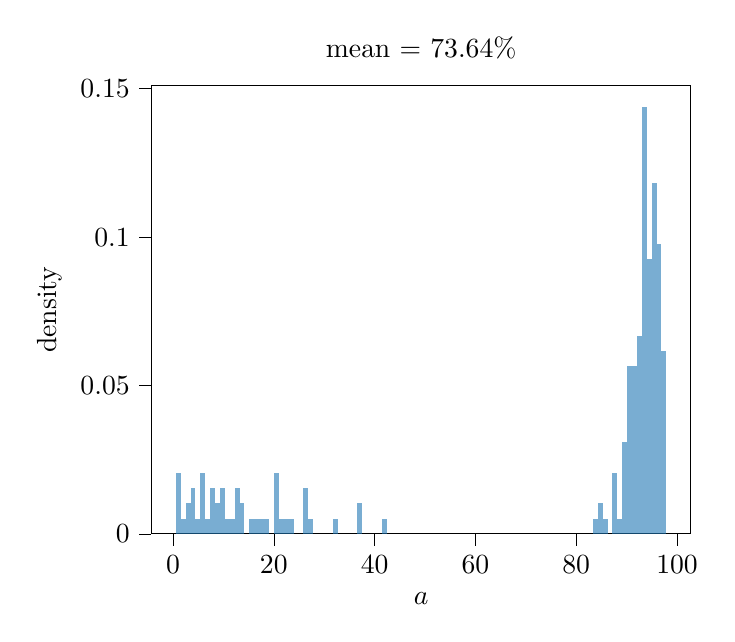
\begin{tikzpicture}

\definecolor{color0}{rgb}{0.12156862745098,0.466666666666667,0.705882352941177}

\begin{axis}[
tick align=outside,
tick pos=left,
title={mean = 73.64\%},
xlabel = $a$,
ylabel = density,
x grid style={white!69.0196078431373!black},
xmin=-4.29979344454833, xmax=102.750450824271,
xtick style={color=black},
y grid style={white!69.0196078431373!black},
ymin=0, ymax=0.151050566119165,
ytick style={color=black},
yticklabel style={
        /pgf/number format/fixed,
        /pgf/number format/precision=5
},
scaled y ticks=false
]
\draw[draw=none,fill=color0,fill opacity=0.6] (axis cs:0.566126749488902,0) rectangle (axis cs:1.53931078829635,0.0205510974311789);
\draw[draw=none,fill=color0,fill opacity=0.6] (axis cs:1.53931078829635,0) rectangle (axis cs:2.5124948271038,0.00513777435779472);
\draw[draw=none,fill=color0,fill opacity=0.6] (axis cs:2.5124948271038,0) rectangle (axis cs:3.48567886591124,0.0102755487155894);
\draw[draw=none,fill=color0,fill opacity=0.6] (axis cs:3.48567886591124,0) rectangle (axis cs:4.45886290471869,0.0154133230733842);
\draw[draw=none,fill=color0,fill opacity=0.6] (axis cs:4.45886290471869,0) rectangle (axis cs:5.43204694352614,0.00513777435779472);
\draw[draw=none,fill=color0,fill opacity=0.6] (axis cs:5.43204694352614,0) rectangle (axis cs:6.40523098233358,0.0205510974311789);
\draw[draw=none,fill=color0,fill opacity=0.6] (axis cs:6.40523098233358,0) rectangle (axis cs:7.37841502114103,0.00513777435779472);
\draw[draw=none,fill=color0,fill opacity=0.6] (axis cs:7.37841502114103,0) rectangle (axis cs:8.35159905994848,0.0154133230733842);
\draw[draw=none,fill=color0,fill opacity=0.6] (axis cs:8.35159905994848,0) rectangle (axis cs:9.32478309875592,0.0102755487155894);
\draw[draw=none,fill=color0,fill opacity=0.6] (axis cs:9.32478309875592,0) rectangle (axis cs:10.2979671375634,0.0154133230733841);
\draw[draw=none,fill=color0,fill opacity=0.6] (axis cs:10.2979671375634,0) rectangle (axis cs:11.2711511763708,0.00513777435779471);
\draw[draw=none,fill=color0,fill opacity=0.6] (axis cs:11.2711511763708,0) rectangle (axis cs:12.2443352151783,0.00513777435779472);
\draw[draw=none,fill=color0,fill opacity=0.6] (axis cs:12.2443352151783,0) rectangle (axis cs:13.2175192539857,0.0154133230733842);
\draw[draw=none,fill=color0,fill opacity=0.6] (axis cs:13.2175192539857,0) rectangle (axis cs:14.1907032927932,0.0102755487155894);
\draw[draw=none,fill=color0,fill opacity=0.6] (axis cs:14.1907032927932,0) rectangle (axis cs:15.1638873316006,0);
\draw[draw=none,fill=color0,fill opacity=0.6] (axis cs:15.1638873316006,0) rectangle (axis cs:16.1370713704081,0.00513777435779472);
\draw[draw=none,fill=color0,fill opacity=0.6] (axis cs:16.1370713704081,0) rectangle (axis cs:17.1102554092155,0.00513777435779472);
\draw[draw=none,fill=color0,fill opacity=0.6] (axis cs:17.1102554092155,0) rectangle (axis cs:18.0834394480229,0.00513777435779472);
\draw[draw=none,fill=color0,fill opacity=0.6] (axis cs:18.0834394480229,0) rectangle (axis cs:19.0566234868304,0.0051377743577947);
\draw[draw=none,fill=color0,fill opacity=0.6] (axis cs:19.0566234868304,0) rectangle (axis cs:20.0298075256378,0);
\draw[draw=none,fill=color0,fill opacity=0.6] (axis cs:20.0298075256378,0) rectangle (axis cs:21.0029915644453,0.0205510974311789);
\draw[draw=none,fill=color0,fill opacity=0.6] (axis cs:21.0029915644453,0) rectangle (axis cs:21.9761756032527,0.0051377743577947);
\draw[draw=none,fill=color0,fill opacity=0.6] (axis cs:21.9761756032527,0) rectangle (axis cs:22.9493596420602,0.00513777435779472);
\draw[draw=none,fill=color0,fill opacity=0.6] (axis cs:22.9493596420602,0) rectangle (axis cs:23.9225436808676,0.00513777435779472);
\draw[draw=none,fill=color0,fill opacity=0.6] (axis cs:23.9225436808676,0) rectangle (axis cs:24.8957277196751,0);
\draw[draw=none,fill=color0,fill opacity=0.6] (axis cs:24.8957277196751,0) rectangle (axis cs:25.8689117584825,0);
\draw[draw=none,fill=color0,fill opacity=0.6] (axis cs:25.8689117584825,0) rectangle (axis cs:26.84209579729,0.0154133230733841);
\draw[draw=none,fill=color0,fill opacity=0.6] (axis cs:26.84209579729,0) rectangle (axis cs:27.8152798360974,0.00513777435779472);
\draw[draw=none,fill=color0,fill opacity=0.6] (axis cs:27.8152798360974,0) rectangle (axis cs:28.7884638749049,0);
\draw[draw=none,fill=color0,fill opacity=0.6] (axis cs:28.7884638749049,0) rectangle (axis cs:29.7616479137123,0);
\draw[draw=none,fill=color0,fill opacity=0.6] (axis cs:29.7616479137123,0) rectangle (axis cs:30.7348319525198,0);
\draw[draw=none,fill=color0,fill opacity=0.6] (axis cs:30.7348319525198,0) rectangle (axis cs:31.7080159913272,0);
\draw[draw=none,fill=color0,fill opacity=0.6] (axis cs:31.7080159913272,0) rectangle (axis cs:32.6812000301346,0.00513777435779472);
\draw[draw=none,fill=color0,fill opacity=0.6] (axis cs:32.6812000301346,0) rectangle (axis cs:33.6543840689421,0);
\draw[draw=none,fill=color0,fill opacity=0.6] (axis cs:33.6543840689421,0) rectangle (axis cs:34.6275681077495,0);
\draw[draw=none,fill=color0,fill opacity=0.6] (axis cs:34.6275681077495,0) rectangle (axis cs:35.600752146557,0);
\draw[draw=none,fill=color0,fill opacity=0.6] (axis cs:35.600752146557,0) rectangle (axis cs:36.5739361853644,0);
\draw[draw=none,fill=color0,fill opacity=0.6] (axis cs:36.5739361853644,0) rectangle (axis cs:37.5471202241719,0.0102755487155894);
\draw[draw=none,fill=color0,fill opacity=0.6] (axis cs:37.5471202241719,0) rectangle (axis cs:38.5203042629793,0);
\draw[draw=none,fill=color0,fill opacity=0.6] (axis cs:38.5203042629793,0) rectangle (axis cs:39.4934883017868,0);
\draw[draw=none,fill=color0,fill opacity=0.6] (axis cs:39.4934883017868,0) rectangle (axis cs:40.4666723405942,0);
\draw[draw=none,fill=color0,fill opacity=0.6] (axis cs:40.4666723405942,0) rectangle (axis cs:41.4398563794017,0);
\draw[draw=none,fill=color0,fill opacity=0.6] (axis cs:41.4398563794017,0) rectangle (axis cs:42.4130404182091,0.00513777435779472);
\draw[draw=none,fill=color0,fill opacity=0.6] (axis cs:42.4130404182091,0) rectangle (axis cs:43.3862244570166,0);
\draw[draw=none,fill=color0,fill opacity=0.6] (axis cs:43.3862244570166,0) rectangle (axis cs:44.359408495824,0);
\draw[draw=none,fill=color0,fill opacity=0.6] (axis cs:44.359408495824,0) rectangle (axis cs:45.3325925346315,0);
\draw[draw=none,fill=color0,fill opacity=0.6] (axis cs:45.3325925346315,0) rectangle (axis cs:46.3057765734389,0);
\draw[draw=none,fill=color0,fill opacity=0.6] (axis cs:46.3057765734389,0) rectangle (axis cs:47.2789606122464,0);
\draw[draw=none,fill=color0,fill opacity=0.6] (axis cs:47.2789606122464,0) rectangle (axis cs:48.2521446510538,0);
\draw[draw=none,fill=color0,fill opacity=0.6] (axis cs:48.2521446510538,0) rectangle (axis cs:49.2253286898612,0);
\draw[draw=none,fill=color0,fill opacity=0.6] (axis cs:49.2253286898612,0) rectangle (axis cs:50.1985127286687,0);
\draw[draw=none,fill=color0,fill opacity=0.6] (axis cs:50.1985127286687,0) rectangle (axis cs:51.1716967674761,0);
\draw[draw=none,fill=color0,fill opacity=0.6] (axis cs:51.1716967674761,0) rectangle (axis cs:52.1448808062836,0);
\draw[draw=none,fill=color0,fill opacity=0.6] (axis cs:52.1448808062836,0) rectangle (axis cs:53.118064845091,0);
\draw[draw=none,fill=color0,fill opacity=0.6] (axis cs:53.118064845091,0) rectangle (axis cs:54.0912488838985,0);
\draw[draw=none,fill=color0,fill opacity=0.6] (axis cs:54.0912488838985,0) rectangle (axis cs:55.0644329227059,0);
\draw[draw=none,fill=color0,fill opacity=0.6] (axis cs:55.0644329227059,0) rectangle (axis cs:56.0376169615134,0);
\draw[draw=none,fill=color0,fill opacity=0.6] (axis cs:56.0376169615134,0) rectangle (axis cs:57.0108010003208,0);
\draw[draw=none,fill=color0,fill opacity=0.6] (axis cs:57.0108010003208,0) rectangle (axis cs:57.9839850391283,0);
\draw[draw=none,fill=color0,fill opacity=0.6] (axis cs:57.9839850391283,0) rectangle (axis cs:58.9571690779357,0);
\draw[draw=none,fill=color0,fill opacity=0.6] (axis cs:58.9571690779357,0) rectangle (axis cs:59.9303531167432,0);
\draw[draw=none,fill=color0,fill opacity=0.6] (axis cs:59.9303531167432,0) rectangle (axis cs:60.9035371555506,0);
\draw[draw=none,fill=color0,fill opacity=0.6] (axis cs:60.9035371555506,0) rectangle (axis cs:61.8767211943581,0);
\draw[draw=none,fill=color0,fill opacity=0.6] (axis cs:61.8767211943581,0) rectangle (axis cs:62.8499052331655,0);
\draw[draw=none,fill=color0,fill opacity=0.6] (axis cs:62.8499052331655,0) rectangle (axis cs:63.8230892719729,0);
\draw[draw=none,fill=color0,fill opacity=0.6] (axis cs:63.823089271973,0) rectangle (axis cs:64.7962733107804,0);
\draw[draw=none,fill=color0,fill opacity=0.6] (axis cs:64.7962733107804,0) rectangle (axis cs:65.7694573495878,0);
\draw[draw=none,fill=color0,fill opacity=0.6] (axis cs:65.7694573495878,0) rectangle (axis cs:66.7426413883953,0);
\draw[draw=none,fill=color0,fill opacity=0.6] (axis cs:66.7426413883953,0) rectangle (axis cs:67.7158254272027,0);
\draw[draw=none,fill=color0,fill opacity=0.6] (axis cs:67.7158254272027,0) rectangle (axis cs:68.6890094660102,0);
\draw[draw=none,fill=color0,fill opacity=0.6] (axis cs:68.6890094660102,0) rectangle (axis cs:69.6621935048176,0);
\draw[draw=none,fill=color0,fill opacity=0.6] (axis cs:69.6621935048176,0) rectangle (axis cs:70.6353775436251,0);
\draw[draw=none,fill=color0,fill opacity=0.6] (axis cs:70.6353775436251,0) rectangle (axis cs:71.6085615824325,0);
\draw[draw=none,fill=color0,fill opacity=0.6] (axis cs:71.6085615824325,0) rectangle (axis cs:72.58174562124,0);
\draw[draw=none,fill=color0,fill opacity=0.6] (axis cs:72.58174562124,0) rectangle (axis cs:73.5549296600474,0);
\draw[draw=none,fill=color0,fill opacity=0.6] (axis cs:73.5549296600474,0) rectangle (axis cs:74.5281136988549,0);
\draw[draw=none,fill=color0,fill opacity=0.6] (axis cs:74.5281136988549,0) rectangle (axis cs:75.5012977376623,0);
\draw[draw=none,fill=color0,fill opacity=0.6] (axis cs:75.5012977376623,0) rectangle (axis cs:76.4744817764697,0);
\draw[draw=none,fill=color0,fill opacity=0.6] (axis cs:76.4744817764698,0) rectangle (axis cs:77.4476658152772,0);
\draw[draw=none,fill=color0,fill opacity=0.6] (axis cs:77.4476658152772,0) rectangle (axis cs:78.4208498540846,0);
\draw[draw=none,fill=color0,fill opacity=0.6] (axis cs:78.4208498540847,0) rectangle (axis cs:79.3940338928921,0);
\draw[draw=none,fill=color0,fill opacity=0.6] (axis cs:79.3940338928921,0) rectangle (axis cs:80.3672179316995,0);
\draw[draw=none,fill=color0,fill opacity=0.6] (axis cs:80.3672179316995,0) rectangle (axis cs:81.340401970507,0);
\draw[draw=none,fill=color0,fill opacity=0.6] (axis cs:81.340401970507,0) rectangle (axis cs:82.3135860093144,0);
\draw[draw=none,fill=color0,fill opacity=0.6] (axis cs:82.3135860093144,0) rectangle (axis cs:83.2867700481219,0);
\draw[draw=none,fill=color0,fill opacity=0.6] (axis cs:83.2867700481219,0) rectangle (axis cs:84.2599540869293,0.00513777435779472);
\draw[draw=none,fill=color0,fill opacity=0.6] (axis cs:84.2599540869293,0) rectangle (axis cs:85.2331381257368,0.0102755487155894);
\draw[draw=none,fill=color0,fill opacity=0.6] (axis cs:85.2331381257368,0) rectangle (axis cs:86.2063221645442,0.00513777435779465);
\draw[draw=none,fill=color0,fill opacity=0.6] (axis cs:86.2063221645442,0) rectangle (axis cs:87.1795062033517,0);
\draw[draw=none,fill=color0,fill opacity=0.6] (axis cs:87.1795062033517,0) rectangle (axis cs:88.1526902421591,0.0205510974311789);
\draw[draw=none,fill=color0,fill opacity=0.6] (axis cs:88.1526902421591,0) rectangle (axis cs:89.1258742809666,0.00513777435779472);
\draw[draw=none,fill=color0,fill opacity=0.6] (axis cs:89.1258742809666,0) rectangle (axis cs:90.099058319774,0.0308266461467683);
\draw[draw=none,fill=color0,fill opacity=0.6] (axis cs:90.099058319774,0) rectangle (axis cs:91.0722423585814,0.0565155179357419);
\draw[draw=none,fill=color0,fill opacity=0.6] (axis cs:91.0722423585815,0) rectangle (axis cs:92.0454263973889,0.0565155179357419);
\draw[draw=none,fill=color0,fill opacity=0.6] (axis cs:92.0454263973889,0) rectangle (axis cs:93.0186104361963,0.0667910666513314);
\draw[draw=none,fill=color0,fill opacity=0.6] (axis cs:93.0186104361964,0) rectangle (axis cs:93.9917944750038,0.143857682018252);
\draw[draw=none,fill=color0,fill opacity=0.6] (axis cs:93.9917944750038,0) rectangle (axis cs:94.9649785138112,0.092479938440305);
\draw[draw=none,fill=color0,fill opacity=0.6] (axis cs:94.9649785138112,0) rectangle (axis cs:95.9381625526187,0.118168810229279);
\draw[draw=none,fill=color0,fill opacity=0.6] (axis cs:95.9381625526187,0) rectangle (axis cs:96.9113465914261,0.0976177127980997);
\draw[draw=none,fill=color0,fill opacity=0.6] (axis cs:96.9113465914261,0) rectangle (axis cs:97.8845306302336,0.0616532922935367);
\end{axis}

\end{tikzpicture}

\end{center}
\end{subfigure}
\caption{Occurences of percentages of saved additions in three dimensions.}
\label{fig:saved_additions_3d}
\end{figure}

As we can see in Figure \ref{fig:saved_additions_3d}, while we have a mean percentage of saved additions of about $73\%$ there is actually a majority of cases with $a$-values of more than $90\%$. On the other hand there are a lot of cases with $a$-values below $20\%$. This is remarkable or even surprising, since it looks like our examples more or less fall into two categories in three dimensions. Namely one, where almost all the work is done on the tails of apparent pairs, and one where almost none of the work is done on the tails of apparent pairs. However this behaviour does not occur in two dimensions as Figure \ref{fig:saved_additions_2d} illustrates. Note in particular that the values on the $x$-axis only go from $55$ to $90$ and not from $0$ to $100$ as in \ref{fig:saved_additions_3d}.

\begin{figure}[H]
%\centering%
\begin{subfigure}[c]{0.95\textwidth}
\begin{center}
% This file was created by tikzplotlib v0.9.2.
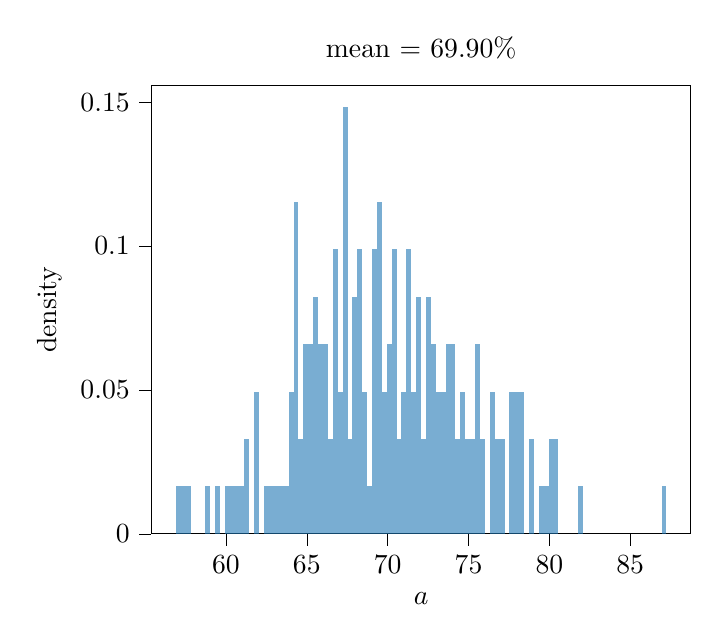
\begin{tikzpicture}

\definecolor{color0}{rgb}{0.12156862745098,0.466666666666667,0.705882352941177}

\begin{axis}[
tick align=outside,
tick pos=left,
title={mean = 69.90\%},
x grid style={white!69.0196078431373!black},
xmin=55.3829134003992, xmax=88.7546598014462,
xtick style={color=black},
yticklabel style={
        /pgf/number format/fixed,
        /pgf/number format/precision=5
},
xlabel = $a$,
ylabel = density,
scaled y ticks=false,
y grid style={white!69.0196078431373!black},
ymin=0, ymax=0.155745520103709,
ytick style={color=black}
]
\draw[draw=none,fill=color0,fill opacity=0.6] (axis cs:56.8998109640832,0) rectangle (axis cs:57.20319047682,0.0164810074183815);
\draw[draw=none,fill=color0,fill opacity=0.6] (axis cs:57.20319047682,0) rectangle (axis cs:57.5065699895567,0.0164810074183815);
\draw[draw=none,fill=color0,fill opacity=0.6] (axis cs:57.5065699895568,0) rectangle (axis cs:57.8099495022935,0.0164810074183815);
\draw[draw=none,fill=color0,fill opacity=0.6] (axis cs:57.8099495022935,0) rectangle (axis cs:58.1133290150303,0);
\draw[draw=none,fill=color0,fill opacity=0.6] (axis cs:58.1133290150303,0) rectangle (axis cs:58.4167085277671,0);
\draw[draw=none,fill=color0,fill opacity=0.6] (axis cs:58.4167085277671,0) rectangle (axis cs:58.7200880405039,0);
\draw[draw=none,fill=color0,fill opacity=0.6] (axis cs:58.7200880405039,0) rectangle (axis cs:59.0234675532407,0.0164810074183815);
\draw[draw=none,fill=color0,fill opacity=0.6] (axis cs:59.0234675532407,0) rectangle (axis cs:59.3268470659775,0);
\draw[draw=none,fill=color0,fill opacity=0.6] (axis cs:59.3268470659775,0) rectangle (axis cs:59.6302265787143,0.0164810074183815);
\draw[draw=none,fill=color0,fill opacity=0.6] (axis cs:59.6302265787143,0) rectangle (axis cs:59.9336060914511,0);
\draw[draw=none,fill=color0,fill opacity=0.6] (axis cs:59.9336060914511,0) rectangle (axis cs:60.2369856041879,0.0164810074183815);
\draw[draw=none,fill=color0,fill opacity=0.6] (axis cs:60.2369856041879,0) rectangle (axis cs:60.5403651169247,0.0164810074183815);
\draw[draw=none,fill=color0,fill opacity=0.6] (axis cs:60.5403651169247,0) rectangle (axis cs:60.8437446296615,0.0164810074183815);
\draw[draw=none,fill=color0,fill opacity=0.6] (axis cs:60.8437446296614,0) rectangle (axis cs:61.1471241423982,0.0164810074183815);
\draw[draw=none,fill=color0,fill opacity=0.6] (axis cs:61.1471241423982,0) rectangle (axis cs:61.450503655135,0.032962014836763);
\draw[draw=none,fill=color0,fill opacity=0.6] (axis cs:61.450503655135,0) rectangle (axis cs:61.7538831678718,0);
\draw[draw=none,fill=color0,fill opacity=0.6] (axis cs:61.7538831678718,0) rectangle (axis cs:62.0572626806086,0.0494430222551434);
\draw[draw=none,fill=color0,fill opacity=0.6] (axis cs:62.0572626806086,0) rectangle (axis cs:62.3606421933454,0);
\draw[draw=none,fill=color0,fill opacity=0.6] (axis cs:62.3606421933454,0) rectangle (axis cs:62.6640217060822,0.0164810074183815);
\draw[draw=none,fill=color0,fill opacity=0.6] (axis cs:62.6640217060822,0) rectangle (axis cs:62.967401218819,0.0164810074183815);
\draw[draw=none,fill=color0,fill opacity=0.6] (axis cs:62.967401218819,0) rectangle (axis cs:63.2707807315558,0.0164810074183815);
\draw[draw=none,fill=color0,fill opacity=0.6] (axis cs:63.2707807315558,0) rectangle (axis cs:63.5741602442926,0.0164810074183811);
\draw[draw=none,fill=color0,fill opacity=0.6] (axis cs:63.5741602442926,0) rectangle (axis cs:63.8775397570294,0.0164810074183815);
\draw[draw=none,fill=color0,fill opacity=0.6] (axis cs:63.8775397570294,0) rectangle (axis cs:64.1809192697662,0.0494430222551446);
\draw[draw=none,fill=color0,fill opacity=0.6] (axis cs:64.1809192697662,0) rectangle (axis cs:64.4842987825029,0.115367051928673);
\draw[draw=none,fill=color0,fill opacity=0.6] (axis cs:64.4842987825029,0) rectangle (axis cs:64.7876782952397,0.0329620148367623);
\draw[draw=none,fill=color0,fill opacity=0.6] (axis cs:64.7876782952397,0) rectangle (axis cs:65.0910578079765,0.0659240296735246);
\draw[draw=none,fill=color0,fill opacity=0.6] (axis cs:65.0910578079765,0) rectangle (axis cs:65.3944373207133,0.0659240296735276);
\draw[draw=none,fill=color0,fill opacity=0.6] (axis cs:65.3944373207133,0) rectangle (axis cs:65.6978168334501,0.0824050370919057);
\draw[draw=none,fill=color0,fill opacity=0.6] (axis cs:65.6978168334501,0) rectangle (axis cs:66.0011963461869,0.0659240296735276);
\draw[draw=none,fill=color0,fill opacity=0.6] (axis cs:66.0011963461869,0) rectangle (axis cs:66.3045758589237,0.0659240296735246);
\draw[draw=none,fill=color0,fill opacity=0.6] (axis cs:66.3045758589237,0) rectangle (axis cs:66.6079553716605,0.0329620148367638);
\draw[draw=none,fill=color0,fill opacity=0.6] (axis cs:66.6079553716605,0) rectangle (axis cs:66.9113348843973,0.0988860445102868);
\draw[draw=none,fill=color0,fill opacity=0.6] (axis cs:66.9113348843973,0) rectangle (axis cs:67.2147143971341,0.0494430222551434);
\draw[draw=none,fill=color0,fill opacity=0.6] (axis cs:67.2147143971341,0) rectangle (axis cs:67.5180939098708,0.148329066765437);
\draw[draw=none,fill=color0,fill opacity=0.6] (axis cs:67.5180939098708,0) rectangle (axis cs:67.8214734226076,0.0329620148367623);
\draw[draw=none,fill=color0,fill opacity=0.6] (axis cs:67.8214734226076,0) rectangle (axis cs:68.1248529353444,0.0824050370919095);
\draw[draw=none,fill=color0,fill opacity=0.6] (axis cs:68.1248529353444,0) rectangle (axis cs:68.4282324480812,0.0988860445102868);
\draw[draw=none,fill=color0,fill opacity=0.6] (axis cs:68.4282324480812,0) rectangle (axis cs:68.731611960818,0.0494430222551434);
\draw[draw=none,fill=color0,fill opacity=0.6] (axis cs:68.731611960818,0) rectangle (axis cs:69.0349914735548,0.0164810074183819);
\draw[draw=none,fill=color0,fill opacity=0.6] (axis cs:69.0349914735548,0) rectangle (axis cs:69.3383709862916,0.0988860445102868);
\draw[draw=none,fill=color0,fill opacity=0.6] (axis cs:69.3383709862916,0) rectangle (axis cs:69.6417504990284,0.115367051928673);
\draw[draw=none,fill=color0,fill opacity=0.6] (axis cs:69.6417504990284,0) rectangle (axis cs:69.9451300117652,0.0494430222551434);
\draw[draw=none,fill=color0,fill opacity=0.6] (axis cs:69.9451300117652,0) rectangle (axis cs:70.248509524502,0.0659240296735246);
\draw[draw=none,fill=color0,fill opacity=0.6] (axis cs:70.248509524502,0) rectangle (axis cs:70.5518890372388,0.0988860445102915);
\draw[draw=none,fill=color0,fill opacity=0.6] (axis cs:70.5518890372388,0) rectangle (axis cs:70.8552685499755,0.0329620148367623);
\draw[draw=none,fill=color0,fill opacity=0.6] (axis cs:70.8552685499755,0) rectangle (axis cs:71.1586480627123,0.0494430222551457);
\draw[draw=none,fill=color0,fill opacity=0.6] (axis cs:71.1586480627123,0) rectangle (axis cs:71.4620275754491,0.0988860445102868);
\draw[draw=none,fill=color0,fill opacity=0.6] (axis cs:71.4620275754491,0) rectangle (axis cs:71.7654070881859,0.0494430222551457);
\draw[draw=none,fill=color0,fill opacity=0.6] (axis cs:71.7654070881859,0) rectangle (axis cs:72.0687866009227,0.0824050370919057);
\draw[draw=none,fill=color0,fill opacity=0.6] (axis cs:72.0687866009227,0) rectangle (axis cs:72.3721661136595,0.0329620148367638);
\draw[draw=none,fill=color0,fill opacity=0.6] (axis cs:72.3721661136595,0) rectangle (axis cs:72.6755456263963,0.0824050370919057);
\draw[draw=none,fill=color0,fill opacity=0.6] (axis cs:72.6755456263963,0) rectangle (axis cs:72.9789251391331,0.0659240296735246);
\draw[draw=none,fill=color0,fill opacity=0.6] (axis cs:72.9789251391331,0) rectangle (axis cs:73.2823046518699,0.0494430222551457);
\draw[draw=none,fill=color0,fill opacity=0.6] (axis cs:73.2823046518699,0) rectangle (axis cs:73.5856841646067,0.0494430222551434);
\draw[draw=none,fill=color0,fill opacity=0.6] (axis cs:73.5856841646066,0) rectangle (axis cs:73.8890636773434,0.0659240296735276);
\draw[draw=none,fill=color0,fill opacity=0.6] (axis cs:73.8890636773434,0) rectangle (axis cs:74.1924431900802,0.0659240296735246);
\draw[draw=none,fill=color0,fill opacity=0.6] (axis cs:74.1924431900802,0) rectangle (axis cs:74.495822702817,0.0329620148367623);
\draw[draw=none,fill=color0,fill opacity=0.6] (axis cs:74.495822702817,0) rectangle (axis cs:74.7992022155538,0.0494430222551457);
\draw[draw=none,fill=color0,fill opacity=0.6] (axis cs:74.7992022155538,0) rectangle (axis cs:75.1025817282906,0.0329620148367623);
\draw[draw=none,fill=color0,fill opacity=0.6] (axis cs:75.1025817282906,0) rectangle (axis cs:75.4059612410274,0.0329620148367638);
\draw[draw=none,fill=color0,fill opacity=0.6] (axis cs:75.4059612410274,0) rectangle (axis cs:75.7093407537642,0.0659240296735246);
\draw[draw=none,fill=color0,fill opacity=0.6] (axis cs:75.7093407537642,0) rectangle (axis cs:76.012720266501,0.0329620148367623);
\draw[draw=none,fill=color0,fill opacity=0.6] (axis cs:76.012720266501,0) rectangle (axis cs:76.3160997792378,0);
\draw[draw=none,fill=color0,fill opacity=0.6] (axis cs:76.3160997792378,0) rectangle (axis cs:76.6194792919745,0.0494430222551457);
\draw[draw=none,fill=color0,fill opacity=0.6] (axis cs:76.6194792919746,0) rectangle (axis cs:76.9228588047114,0.0329620148367623);
\draw[draw=none,fill=color0,fill opacity=0.6] (axis cs:76.9228588047114,0) rectangle (axis cs:77.2262383174481,0.0329620148367623);
\draw[draw=none,fill=color0,fill opacity=0.6] (axis cs:77.2262383174481,0) rectangle (axis cs:77.5296178301849,0);
\draw[draw=none,fill=color0,fill opacity=0.6] (axis cs:77.5296178301849,0) rectangle (axis cs:77.8329973429217,0.0494430222551434);
\draw[draw=none,fill=color0,fill opacity=0.6] (axis cs:77.8329973429217,0) rectangle (axis cs:78.1363768556585,0.0494430222551457);
\draw[draw=none,fill=color0,fill opacity=0.6] (axis cs:78.1363768556585,0) rectangle (axis cs:78.4397563683953,0.0494430222551434);
\draw[draw=none,fill=color0,fill opacity=0.6] (axis cs:78.4397563683953,0) rectangle (axis cs:78.7431358811321,0);
\draw[draw=none,fill=color0,fill opacity=0.6] (axis cs:78.7431358811321,0) rectangle (axis cs:79.0465153938689,0.0329620148367638);
\draw[draw=none,fill=color0,fill opacity=0.6] (axis cs:79.0465153938689,0) rectangle (axis cs:79.3498949066057,0);
\draw[draw=none,fill=color0,fill opacity=0.6] (axis cs:79.3498949066057,0) rectangle (axis cs:79.6532744193425,0.0164810074183819);
\draw[draw=none,fill=color0,fill opacity=0.6] (axis cs:79.6532744193425,0) rectangle (axis cs:79.9566539320793,0.0164810074183811);
\draw[draw=none,fill=color0,fill opacity=0.6] (axis cs:79.9566539320793,0) rectangle (axis cs:80.2600334448161,0.0329620148367623);
\draw[draw=none,fill=color0,fill opacity=0.6] (axis cs:80.2600334448161,0) rectangle (axis cs:80.5634129575528,0.0329620148367638);
\draw[draw=none,fill=color0,fill opacity=0.6] (axis cs:80.5634129575528,0) rectangle (axis cs:80.8667924702896,0);
\draw[draw=none,fill=color0,fill opacity=0.6] (axis cs:80.8667924702896,0) rectangle (axis cs:81.1701719830264,0);
\draw[draw=none,fill=color0,fill opacity=0.6] (axis cs:81.1701719830264,0) rectangle (axis cs:81.4735514957632,0);
\draw[draw=none,fill=color0,fill opacity=0.6] (axis cs:81.4735514957632,0) rectangle (axis cs:81.7769310085,0);
\draw[draw=none,fill=color0,fill opacity=0.6] (axis cs:81.7769310085,0) rectangle (axis cs:82.0803105212368,0.0164810074183819);
\draw[draw=none,fill=color0,fill opacity=0.6] (axis cs:82.0803105212368,0) rectangle (axis cs:82.3836900339736,0);
\draw[draw=none,fill=color0,fill opacity=0.6] (axis cs:82.3836900339736,0) rectangle (axis cs:82.6870695467104,0);
\draw[draw=none,fill=color0,fill opacity=0.6] (axis cs:82.6870695467104,0) rectangle (axis cs:82.9904490594472,0);
\draw[draw=none,fill=color0,fill opacity=0.6] (axis cs:82.9904490594472,0) rectangle (axis cs:83.293828572184,0);
\draw[draw=none,fill=color0,fill opacity=0.6] (axis cs:83.293828572184,0) rectangle (axis cs:83.5972080849208,0);
\draw[draw=none,fill=color0,fill opacity=0.6] (axis cs:83.5972080849207,0) rectangle (axis cs:83.9005875976575,0);
\draw[draw=none,fill=color0,fill opacity=0.6] (axis cs:83.9005875976575,0) rectangle (axis cs:84.2039671103943,0);
\draw[draw=none,fill=color0,fill opacity=0.6] (axis cs:84.2039671103943,0) rectangle (axis cs:84.5073466231311,0);
\draw[draw=none,fill=color0,fill opacity=0.6] (axis cs:84.5073466231311,0) rectangle (axis cs:84.8107261358679,0);
\draw[draw=none,fill=color0,fill opacity=0.6] (axis cs:84.8107261358679,0) rectangle (axis cs:85.1141056486047,0);
\draw[draw=none,fill=color0,fill opacity=0.6] (axis cs:85.1141056486047,0) rectangle (axis cs:85.4174851613415,0);
\draw[draw=none,fill=color0,fill opacity=0.6] (axis cs:85.4174851613415,0) rectangle (axis cs:85.7208646740783,0);
\draw[draw=none,fill=color0,fill opacity=0.6] (axis cs:85.7208646740783,0) rectangle (axis cs:86.0242441868151,0);
\draw[draw=none,fill=color0,fill opacity=0.6] (axis cs:86.0242441868151,0) rectangle (axis cs:86.3276236995519,0);
\draw[draw=none,fill=color0,fill opacity=0.6] (axis cs:86.3276236995519,0) rectangle (axis cs:86.6310032122887,0);
\draw[draw=none,fill=color0,fill opacity=0.6] (axis cs:86.6310032122886,0) rectangle (axis cs:86.9343827250254,0);
\draw[draw=none,fill=color0,fill opacity=0.6] (axis cs:86.9343827250254,0) rectangle (axis cs:87.2377622377622,0.0164810074183811);
\end{axis}

\end{tikzpicture}

\end{center}
\end{subfigure}
\caption{Occurences of percentages of saved additions in two dimensions.}
\label{fig:saved_additions_2d}
\end{figure}

Similar behavior showed for point clouds drawn from the uniform distribution and the Gaussian mixture. However, when increasing the number of points in three dimensions the distribution of $a$-values changes. Consider the following figure.

\begin{figure}[H]
%\centering%
\begin{subfigure}[c]{0.95\textwidth}
\begin{center}
% This file was created by tikzplotlib v0.9.2.
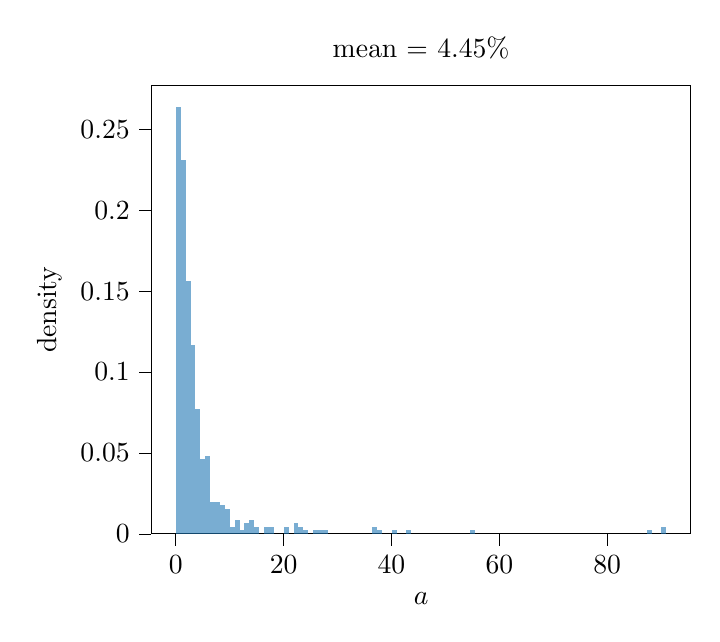
\begin{tikzpicture}

\definecolor{color0}{rgb}{0.12156862745098,0.466666666666667,0.705882352941177}

\begin{axis}[
tick align=outside,
tick pos=left,
title={mean = 4.45\%},
xlabel = $a$,
ylabel = density,
x grid style={white!69.0196078431373!black},
xmin=-4.53430785783378, xmax=95.5162073032124,
xtick style={color=black},
y grid style={white!69.0196078431373!black},
yticklabel style={
        /pgf/number format/fixed,
        /pgf/number format/precision=5
},
scaled y ticks=false,
ymin=0, ymax=0.277060042673249,
ytick style={color=black}
]
\draw[draw=none,fill=color0,fill opacity=0.6] (axis cs:0.0134428313046868,0) rectangle (axis cs:0.922992969132379,0.263866707307856);
\draw[draw=none,fill=color0,fill opacity=0.6] (axis cs:0.922992969132379,0) rectangle (axis cs:1.83254310696007,0.230883368894374);
\draw[draw=none,fill=color0,fill opacity=0.6] (axis cs:1.83254310696007,0) rectangle (axis cs:2.74209324478776,0.156121135157148);
\draw[draw=none,fill=color0,fill opacity=0.6] (axis cs:2.74209324478776,0) rectangle (axis cs:3.65164338261546,0.11654112906097);
\draw[draw=none,fill=color0,fill opacity=0.6] (axis cs:3.65164338261546,0) rectangle (axis cs:4.56119352044315,0.0769611229647914);
\draw[draw=none,fill=color0,fill opacity=0.6] (axis cs:4.56119352044315,0) rectangle (axis cs:5.47074365827084,0.0461766737788748);
\draw[draw=none,fill=color0,fill opacity=0.6] (axis cs:5.47074365827084,0) rectangle (axis cs:6.38029379609854,0.0483755630064403);
\draw[draw=none,fill=color0,fill opacity=0.6] (axis cs:6.38029379609853,0) rectangle (axis cs:7.28984393392623,0.0197900030480892);
\draw[draw=none,fill=color0,fill opacity=0.6] (axis cs:7.28984393392623,0) rectangle (axis cs:8.19939407175392,0.0197900030480892);
\draw[draw=none,fill=color0,fill opacity=0.6] (axis cs:8.19939407175392,0) rectangle (axis cs:9.10894420958161,0.0175911138205238);
\draw[draw=none,fill=color0,fill opacity=0.6] (axis cs:9.10894420958161,0) rectangle (axis cs:10.0184943474093,0.0153922245929583);
\draw[draw=none,fill=color0,fill opacity=0.6] (axis cs:10.0184943474093,0) rectangle (axis cs:10.928044485237,0.00439777845513093);
\draw[draw=none,fill=color0,fill opacity=0.6] (axis cs:10.928044485237,0) rectangle (axis cs:11.8375946230647,0.00879555691026186);
\draw[draw=none,fill=color0,fill opacity=0.6] (axis cs:11.8375946230647,0) rectangle (axis cs:12.7471447608924,0.00219888922756547);
\draw[draw=none,fill=color0,fill opacity=0.6] (axis cs:12.7471447608924,0) rectangle (axis cs:13.6566948987201,0.00659666768269641);
\draw[draw=none,fill=color0,fill opacity=0.6] (axis cs:13.6566948987201,0) rectangle (axis cs:14.5662450365478,0.00879555691026186);
\draw[draw=none,fill=color0,fill opacity=0.6] (axis cs:14.5662450365478,0) rectangle (axis cs:15.4757951743755,0.00439777845513093);
\draw[draw=none,fill=color0,fill opacity=0.6] (axis cs:15.4757951743755,0) rectangle (axis cs:16.3853453122032,0);
\draw[draw=none,fill=color0,fill opacity=0.6] (axis cs:16.3853453122032,0) rectangle (axis cs:17.2948954500308,0.00439777845513095);
\draw[draw=none,fill=color0,fill opacity=0.6] (axis cs:17.2948954500308,0) rectangle (axis cs:18.2044455878585,0.00439777845513093);
\draw[draw=none,fill=color0,fill opacity=0.6] (axis cs:18.2044455878585,0) rectangle (axis cs:19.1139957256862,0);
\draw[draw=none,fill=color0,fill opacity=0.6] (axis cs:19.1139957256862,0) rectangle (axis cs:20.0235458635139,0);
\draw[draw=none,fill=color0,fill opacity=0.6] (axis cs:20.0235458635139,0) rectangle (axis cs:20.9330960013416,0.00439777845513093);
\draw[draw=none,fill=color0,fill opacity=0.6] (axis cs:20.9330960013416,0) rectangle (axis cs:21.8426461391693,0);
\draw[draw=none,fill=color0,fill opacity=0.6] (axis cs:21.8426461391693,0) rectangle (axis cs:22.752196276997,0.0065966676826964);
\draw[draw=none,fill=color0,fill opacity=0.6] (axis cs:22.752196276997,0) rectangle (axis cs:23.6617464148247,0.00439777845513093);
\draw[draw=none,fill=color0,fill opacity=0.6] (axis cs:23.6617464148247,0) rectangle (axis cs:24.5712965526524,0.00219888922756547);
\draw[draw=none,fill=color0,fill opacity=0.6] (axis cs:24.5712965526524,0) rectangle (axis cs:25.4808466904801,0);
\draw[draw=none,fill=color0,fill opacity=0.6] (axis cs:25.4808466904801,0) rectangle (axis cs:26.3903968283078,0.00219888922756547);
\draw[draw=none,fill=color0,fill opacity=0.6] (axis cs:26.3903968283078,0) rectangle (axis cs:27.2999469661355,0.00219888922756547);
\draw[draw=none,fill=color0,fill opacity=0.6] (axis cs:27.2999469661355,0) rectangle (axis cs:28.2094971039632,0.00219888922756547);
\draw[draw=none,fill=color0,fill opacity=0.6] (axis cs:28.2094971039632,0) rectangle (axis cs:29.1190472417909,0);
\draw[draw=none,fill=color0,fill opacity=0.6] (axis cs:29.1190472417909,0) rectangle (axis cs:30.0285973796185,0);
\draw[draw=none,fill=color0,fill opacity=0.6] (axis cs:30.0285973796185,0) rectangle (axis cs:30.9381475174462,0);
\draw[draw=none,fill=color0,fill opacity=0.6] (axis cs:30.9381475174462,0) rectangle (axis cs:31.8476976552739,0);
\draw[draw=none,fill=color0,fill opacity=0.6] (axis cs:31.8476976552739,0) rectangle (axis cs:32.7572477931016,0);
\draw[draw=none,fill=color0,fill opacity=0.6] (axis cs:32.7572477931016,0) rectangle (axis cs:33.6667979309293,0);
\draw[draw=none,fill=color0,fill opacity=0.6] (axis cs:33.6667979309293,0) rectangle (axis cs:34.576348068757,0);
\draw[draw=none,fill=color0,fill opacity=0.6] (axis cs:34.576348068757,0) rectangle (axis cs:35.4858982065847,0);
\draw[draw=none,fill=color0,fill opacity=0.6] (axis cs:35.4858982065847,0) rectangle (axis cs:36.3954483444124,0);
\draw[draw=none,fill=color0,fill opacity=0.6] (axis cs:36.3954483444124,0) rectangle (axis cs:37.3049984822401,0.00439777845513093);
\draw[draw=none,fill=color0,fill opacity=0.6] (axis cs:37.3049984822401,0) rectangle (axis cs:38.2145486200678,0.00219888922756547);
\draw[draw=none,fill=color0,fill opacity=0.6] (axis cs:38.2145486200678,0) rectangle (axis cs:39.1240987578955,0);
\draw[draw=none,fill=color0,fill opacity=0.6] (axis cs:39.1240987578955,0) rectangle (axis cs:40.0336488957232,0);
\draw[draw=none,fill=color0,fill opacity=0.6] (axis cs:40.0336488957232,0) rectangle (axis cs:40.9431990335509,0.00219888922756547);
\draw[draw=none,fill=color0,fill opacity=0.6] (axis cs:40.9431990335509,0) rectangle (axis cs:41.8527491713785,0);
\draw[draw=none,fill=color0,fill opacity=0.6] (axis cs:41.8527491713785,0) rectangle (axis cs:42.7622993092062,0);
\draw[draw=none,fill=color0,fill opacity=0.6] (axis cs:42.7622993092062,0) rectangle (axis cs:43.6718494470339,0.00219888922756547);
\draw[draw=none,fill=color0,fill opacity=0.6] (axis cs:43.6718494470339,0) rectangle (axis cs:44.5813995848616,0);
\draw[draw=none,fill=color0,fill opacity=0.6] (axis cs:44.5813995848616,0) rectangle (axis cs:45.4909497226893,0);
\draw[draw=none,fill=color0,fill opacity=0.6] (axis cs:45.4909497226893,0) rectangle (axis cs:46.400499860517,0);
\draw[draw=none,fill=color0,fill opacity=0.6] (axis cs:46.400499860517,0) rectangle (axis cs:47.3100499983447,0);
\draw[draw=none,fill=color0,fill opacity=0.6] (axis cs:47.3100499983447,0) rectangle (axis cs:48.2196001361724,0);
\draw[draw=none,fill=color0,fill opacity=0.6] (axis cs:48.2196001361724,0) rectangle (axis cs:49.1291502740001,0);
\draw[draw=none,fill=color0,fill opacity=0.6] (axis cs:49.1291502740001,0) rectangle (axis cs:50.0387004118278,0);
\draw[draw=none,fill=color0,fill opacity=0.6] (axis cs:50.0387004118278,0) rectangle (axis cs:50.9482505496555,0);
\draw[draw=none,fill=color0,fill opacity=0.6] (axis cs:50.9482505496555,0) rectangle (axis cs:51.8578006874832,0);
\draw[draw=none,fill=color0,fill opacity=0.6] (axis cs:51.8578006874832,0) rectangle (axis cs:52.7673508253109,0);
\draw[draw=none,fill=color0,fill opacity=0.6] (axis cs:52.7673508253109,0) rectangle (axis cs:53.6769009631386,0);
\draw[draw=none,fill=color0,fill opacity=0.6] (axis cs:53.6769009631386,0) rectangle (axis cs:54.5864511009662,0);
\draw[draw=none,fill=color0,fill opacity=0.6] (axis cs:54.5864511009662,0) rectangle (axis cs:55.4960012387939,0.00219888922756547);
\draw[draw=none,fill=color0,fill opacity=0.6] (axis cs:55.4960012387939,0) rectangle (axis cs:56.4055513766216,0);
\draw[draw=none,fill=color0,fill opacity=0.6] (axis cs:56.4055513766216,0) rectangle (axis cs:57.3151015144493,0);
\draw[draw=none,fill=color0,fill opacity=0.6] (axis cs:57.3151015144493,0) rectangle (axis cs:58.224651652277,0);
\draw[draw=none,fill=color0,fill opacity=0.6] (axis cs:58.224651652277,0) rectangle (axis cs:59.1342017901047,0);
\draw[draw=none,fill=color0,fill opacity=0.6] (axis cs:59.1342017901047,0) rectangle (axis cs:60.0437519279324,0);
\draw[draw=none,fill=color0,fill opacity=0.6] (axis cs:60.0437519279324,0) rectangle (axis cs:60.9533020657601,0);
\draw[draw=none,fill=color0,fill opacity=0.6] (axis cs:60.9533020657601,0) rectangle (axis cs:61.8628522035878,0);
\draw[draw=none,fill=color0,fill opacity=0.6] (axis cs:61.8628522035878,0) rectangle (axis cs:62.7724023414155,0);
\draw[draw=none,fill=color0,fill opacity=0.6] (axis cs:62.7724023414155,0) rectangle (axis cs:63.6819524792432,0);
\draw[draw=none,fill=color0,fill opacity=0.6] (axis cs:63.6819524792432,0) rectangle (axis cs:64.5915026170709,0);
\draw[draw=none,fill=color0,fill opacity=0.6] (axis cs:64.5915026170709,0) rectangle (axis cs:65.5010527548986,0);
\draw[draw=none,fill=color0,fill opacity=0.6] (axis cs:65.5010527548986,0) rectangle (axis cs:66.4106028927262,0);
\draw[draw=none,fill=color0,fill opacity=0.6] (axis cs:66.4106028927262,0) rectangle (axis cs:67.3201530305539,0);
\draw[draw=none,fill=color0,fill opacity=0.6] (axis cs:67.3201530305539,0) rectangle (axis cs:68.2297031683816,0);
\draw[draw=none,fill=color0,fill opacity=0.6] (axis cs:68.2297031683816,0) rectangle (axis cs:69.1392533062093,0);
\draw[draw=none,fill=color0,fill opacity=0.6] (axis cs:69.1392533062093,0) rectangle (axis cs:70.048803444037,0);
\draw[draw=none,fill=color0,fill opacity=0.6] (axis cs:70.048803444037,0) rectangle (axis cs:70.9583535818647,0);
\draw[draw=none,fill=color0,fill opacity=0.6] (axis cs:70.9583535818647,0) rectangle (axis cs:71.8679037196924,0);
\draw[draw=none,fill=color0,fill opacity=0.6] (axis cs:71.8679037196924,0) rectangle (axis cs:72.7774538575201,0);
\draw[draw=none,fill=color0,fill opacity=0.6] (axis cs:72.7774538575201,0) rectangle (axis cs:73.6870039953478,0);
\draw[draw=none,fill=color0,fill opacity=0.6] (axis cs:73.6870039953478,0) rectangle (axis cs:74.5965541331755,0);
\draw[draw=none,fill=color0,fill opacity=0.6] (axis cs:74.5965541331755,0) rectangle (axis cs:75.5061042710032,0);
\draw[draw=none,fill=color0,fill opacity=0.6] (axis cs:75.5061042710032,0) rectangle (axis cs:76.4156544088309,0);
\draw[draw=none,fill=color0,fill opacity=0.6] (axis cs:76.4156544088309,0) rectangle (axis cs:77.3252045466586,0);
\draw[draw=none,fill=color0,fill opacity=0.6] (axis cs:77.3252045466586,0) rectangle (axis cs:78.2347546844863,0);
\draw[draw=none,fill=color0,fill opacity=0.6] (axis cs:78.2347546844863,0) rectangle (axis cs:79.144304822314,0);
\draw[draw=none,fill=color0,fill opacity=0.6] (axis cs:79.144304822314,0) rectangle (axis cs:80.0538549601416,0);
\draw[draw=none,fill=color0,fill opacity=0.6] (axis cs:80.0538549601416,0) rectangle (axis cs:80.9634050979693,0);
\draw[draw=none,fill=color0,fill opacity=0.6] (axis cs:80.9634050979693,0) rectangle (axis cs:81.872955235797,0);
\draw[draw=none,fill=color0,fill opacity=0.6] (axis cs:81.872955235797,0) rectangle (axis cs:82.7825053736247,0);
\draw[draw=none,fill=color0,fill opacity=0.6] (axis cs:82.7825053736247,0) rectangle (axis cs:83.6920555114524,0);
\draw[draw=none,fill=color0,fill opacity=0.6] (axis cs:83.6920555114524,0) rectangle (axis cs:84.6016056492801,0);
\draw[draw=none,fill=color0,fill opacity=0.6] (axis cs:84.6016056492801,0) rectangle (axis cs:85.5111557871078,0);
\draw[draw=none,fill=color0,fill opacity=0.6] (axis cs:85.5111557871078,0) rectangle (axis cs:86.4207059249355,0);
\draw[draw=none,fill=color0,fill opacity=0.6] (axis cs:86.4207059249355,0) rectangle (axis cs:87.3302560627632,0);
\draw[draw=none,fill=color0,fill opacity=0.6] (axis cs:87.3302560627632,0) rectangle (axis cs:88.2398062005909,0.00219888922756547);
\draw[draw=none,fill=color0,fill opacity=0.6] (axis cs:88.2398062005909,0) rectangle (axis cs:89.1493563384186,0);
\draw[draw=none,fill=color0,fill opacity=0.6] (axis cs:89.1493563384186,0) rectangle (axis cs:90.0589064762463,0);
\draw[draw=none,fill=color0,fill opacity=0.6] (axis cs:90.0589064762463,0) rectangle (axis cs:90.968456614074,0.00439777845513093);
\end{axis}

\end{tikzpicture}

\end{center}
\end{subfigure}
\caption{Occurences of percentages of saved additions in three dimensions on point clouds of $200$ points.}
\label{fig:saved_additions_3d_large_complex}
\end{figure}

Figure \ref{fig:saved_additions_3d_large_complex} in the vast majority of cases, there are very few additions saved. We still see some rare cases around the $90\%$ mark and some values in between $10\%$ and $60\%$, but we end up with a mean for saved additions of $4.45\%$ which is substantially lower than the $73.64\%$ we saw in Figure~\ref{fig:saved_additions_3d}. Note that all constructed complexes had elements that were part of apparent pairs between $89.5\%$ and $91\%$. Indeed some more detailed analysis in which we split the filtrations into two classes, namely those with $a$-values above and below $50\%$ revealed no other readily accessible differences. The values of the means of the size of the filtrations, the percentage of apparent pairs, and the number of additions needed in the standard reduction without clearing were within $1\%$ of each other for all examples generated on a fixed number of points. 

The following table has the same columns and rows as Table \ref{tab:add_STA_TWI} but this time we are looking at the averaged values of alpha complexes on $300$ points.

 \begin{table}[H]
     \begin{center}
     \begin{tabular}{|c|c|c|c|}
     \hline
     & \multicolumn{3}{|c|}{Percentage of Saved Additions} \\ \cline{1-4}
     Sample distribution & Uniform & Multivariate Normal & Gaussian 		Mixture\\ \hline
     dimension two & 57.53 & 60.63 & 60.91 \\ \hline
     dimension three & 1.58 & 2.21 & 3.73 \\ \hline

     \end{tabular}
     
     \caption{$a$-value for alpha complexes on $300$ points.}
     \label{tab:add_STA_TWI_300}
     \end{center}
 \end{table}
 
As we can see, the percentage of saved additions in dimension two is still significant, while in dimension three it is very small. Assuming that this trend continues as complexes get larger, implies that preprocessing or clearing schemes that implicitly contain the apparent pairs of some filtration generate their speedup outside of them, at least in three dimensions on alpha complexes. This might be of particular interest with respect to the widely used twisted variant of the standard reduction algorithm.

Another interesting thing to note is that again we see bigger improvements for the Gaussian distribution and mixture. But we also know that the average $q$ value in filtrations on $300$ points is lower than for the uniform case. This implies that the percentage of additions saved does not depend on the percentage of elements in apparent pairs but on some structural differences between the filtrations generated on differently sampled point clouds. Furthermore, there is some difference between points drawn from a single or multiple multivariate distributions. This might be within the margin of error for our experiments but might also be caused by structural differences between the two. Further experiments are required to shed further light on this.

\section{Conclusions}
The experiments we considered in this section are initial observations on the relation between apparent gradients, Betti numbers and complicated persistent homology computations that could give an indication in which direction a closer look might yield results.
 
We have seen that the majority of elements in the filtrations we generated by constructing an alpha complex on a random point cloud is part of an apparent pair. Previously, we showed in Chapter \ref{ch:connection} how the reduction of critical cells with respect to an apparent gradient has a lower bound dependent on $V$-paths defined by the apparent pairs. Perhaps it is possible to find descriptions of filtrations based on their apparent gradients that already give us a good indication on whether the filtration will result in expensive or cheap persistent homology computations. A desired result would be a better understanding of why persistent homology computations in practice show linear or slightly super linear growth although the worst case bound is in $\mathcal{O}(n^3)$ \cite{pershom}. 

The behavior of the random discrete Morse function as seen in Figure~\ref{fig:perfect_rdm_v_apparent} is intriguing.

Finally, the partitioning into two classes for three dimensional alpha complexes on few points, as seen in Figure \ref{fig:saved_additions_3d}, might be an interesting starting point for some further analysis. 

